% Submission filename: LoesVanVoorden_2055036_thesis_MSc_DSBE.pdf
% !TeX jobname = LoesVanVoorden_2055036_thesis_MSc_DSBE
% Build from the Thesis/ folder (auxiliary files go to build/):
%   ./compile_thesis.sh
% Or with latexmk:
%   latexmk -pdf LoesVanVoorden_2055036_thesis_MSc_DSBE.tex

\documentclass[12pt, a4paper]{article}

% ── Packages ──────────────────────────────────────────────────────────────────
\usepackage[utf8]{inputenc}
\usepackage[T1]{fontenc}
\usepackage[british]{babel}
\usepackage{tgpagella}  % TeX Gyre Pagella = modern Palatino (matches Tara's thesis font)
\usepackage{geometry}
\geometry{margin=2.5cm}
\linespread{1.3}
\usepackage{hyperref}
\hypersetup{
  pdftitle={Bridging the Explainability Gap: A Framework for Safe Clinical AI using Large Language Model Intermediaries},
  pdfauthor={Loes van Voorden (2055036)},
  pdfsubject={MSc Thesis Data Science in Business and Entrepreneurship},
}
\usepackage[numbers,sort&compress]{natbib}
\bibliographystyle{unsrtnat}
\usepackage{amsmath}
\usepackage{graphicx}
\usepackage{booktabs}
\usepackage{float}
\usepackage{longtable}
\usepackage{array}
\usepackage{xcolor}
\usepackage{tikz}
\usetikzlibrary{positioning}
% ── Visible placeholder box ───────────────────────────────────────────────────
\newcommand{\placeholder}[1]{%
  \vspace{4pt}%
  \noindent\fcolorbox{black!25}{yellow!12}{%
    \parbox{\dimexpr\linewidth-2\fboxsep-2\fboxrule}{%
      \fontsize{8.5}{12}\selectfont\itshape\color{black!60}%
      \textbf{[To be written]} \, #1%
    }%
  }%
  \vspace{4pt}%
}
\usepackage{listings}
\lstdefinestyle{sql}{
  language=SQL,
  basicstyle=\ttfamily\footnotesize,
  keywordstyle=\color{blue!70!black},
  stringstyle=\color{orange!80!black},
  commentstyle=\color{gray}\itshape,
  breaklines=true,
  breakatwhitespace=true,
  frame=single,
  framesep=4pt,
  xleftmargin=8pt,
  xrightmargin=4pt,
  numbers=none,
  showstringspaces=false,
  tabsize=2,
  morekeywords={DATETIME,DATETIME_DIFF,DATETIME_ADD,INTERVAL,STRING_AGG,
                WITH,USING,LIMIT,CROSS,DISTINCT,MIN,MAX,SUM,GROUP,ORDER},
}
\lstdefinestyle{python}{
  language=Python,
  basicstyle=\ttfamily\fontsize{7.5}{10}\selectfont,
  keywordstyle=\color{blue!65!black}\bfseries,
  stringstyle=\color{orange!75!black},
  commentstyle=\color{gray!80!black}\itshape,
  emphstyle=\color{teal!70!black},
  emph={True,False,None,self},
  breaklines=true,
  breakatwhitespace=false,
  keepspaces=true,
  showstringspaces=false,
  tabsize=4,
  frame=tb,
  framesep=5pt,
  rulecolor=\color{black!15},
  xleftmargin=14pt,
  xrightmargin=4pt,
  numbers=left,
  numberstyle=\ttfamily\fontsize{6}{8}\selectfont\color{black!35},
  numbersep=8pt,
  backgroundcolor=\color{black!2},
  lineskip=1pt,
}

% ── Document ──────────────────────────────────────────────────────────────────
\begin{document}

\begin{titlepage}
  \centering
  \vspace*{1.5cm}
  {\Large\bfseries Bridging the Explainability Gap: A Framework for Safe\\
  Clinical AI using Large Language Model Intermediaries\par}
  \vfill
  {\large Loes van Voorden\par}
  \vspace{0.6cm}
  {\normalsize STUDENT NUMBER: 2055036\par}
  \vfill
  \begin{minipage}{\textwidth}
    \centering
    {\normalsize
    \textsc{Thesis submitted in partial fulfillment}\\[0.35em]
    \textsc{of the requirements for the degree of}\\[1.4em]
    \textsc{Master of Science in Data Science in}\\[0.25em]
    \textsc{Business and Entrepreneurship}\\[0.8em]
    \textsc{Jheronimus Academy of Data Science}\par}
  \end{minipage}
  \vfill
  {\normalsize Thesis committee:\par}
  \vspace{0.4cm}
  {\normalsize Dr.\ Danielle Sent\par}
  {\normalsize Dr.\ Martijn Willemsen\par}
  \vfill
  {\normalsize Jheronimus Academy of Data Science\par}
  {\normalsize Den Bosch, The Netherlands\par}
  {\normalsize June 2026\par}
  \vspace*{1.5cm}
\end{titlepage}

\noindent\textbf{Abstract}\par
\vspace{0.6em}
\noindent ICU mortality models perform well but remain difficult for clinicians
to interpret.
Kolmogorov--Arnold Networks (KANs) offer more transparent attributions than
black-box alternatives, yet spline-based visualisations still misalign with
clinical reasoning and can invite causal misinterpretation.
This thesis presents a pipeline that translates KAN outputs into grounded Dutch
narratives via a reasoning LLM, delivered in a three-step web interface with
cognitive forcing and explicit correlational framing.
Explanation artefact quality is validated against the Co-12 framework before
deployment.
A between-subjects study with ICU clinicians compares KAN visualisations alone
against the same visualisations plus the LLM narrative.

\placeholder{State the main clinician-interpretation finding.}

\vspace{1.2em}
\section{Introduction}
% ══════════════════════════════════════════════════════════════════════════════

Artificial intelligence (AI) holds growing promise for improving clinical
decision-making across healthcare. AI systems have been applied to drug
discovery, medical image analysis, and disease diagnosis \citep{topol2019}, 
and estimates suggest that AI adoption in healthcare could reduce expenditure
by \$200--360 billion annually through improved risk stratification and
treatment planning \citep{sahni2023}. Despite this potential, adoption in
clinical practice remains limited. A systematic review of trust in
AI-based clinical decision support systems identified system transparency as
the most consistent barrier: clinicians hesitate to act on recommendations
they cannot understand or verify \citep{tun2025trust}.

This challenge is most acute in high-acuity environments such as the
intensive care unit (ICU), where decisions are time-pressured, consequences
are severe, and patient conditions are complex. Machine Learning (ML) models for
ICU outcome prediction -- including mortality, length of stay, and
complications such as sepsis -- have multiplied in recent years, with a
meta-analysis of 40 studies involving 317,028 patients reporting a pooled
AUC of 0.83 for mortality prediction \citep{sun2025mortality}. Models such
as XGBoost, Random Forest, and gradient boosting machines consistently
outperform traditional scoring systems such as SOFA and APACHE, drawing on
features including age, lactate, vital signs, and ventilation status
\citep{alghatani2024sepsis}. Despite this predictive performance, most
models remain black-box systems whose internal reasoning is opaque to the
clinicians who must act on their outputs \citep{rudin2019stop}. This
opacity is consequential: the adoption of such models in practice remains
limited partly because their outputs frequently fail to support
clinicians' real interpretive tasks, namely sense-making, verification, and
converting a model prediction into an action that is safe and defensible
\citep{ghassemi2021false, tonekaboni2019clinicians}.

In response to this opacity, the field of Explainable Artificial
Intelligence (XAI) has emerged. XAI includes techniques that aim to
make the behaviour and outputs of AI/ML models understandable to human users
\citep{arrieta2020xai, adadi2018peeking}. These techniques fall into two
broad categories. \emph{Post-hoc} methods explain a trained model after
the fact -- for example, SHAP (SHapley Additive exPlanations) and LIME
(Local Interpretable Model-agnostic Explanations) estimate feature
contributions to individual predictions without modifying the model itself
\citep{arrieta2020xai}. \emph{Inherently interpretable} models, by
contrast, are transparent by design: their internal logic can be directly
inspected without a separate explanation layer \citep{rudin2019stop}.
Examples include decision trees, linear models, and more recently,
Kolmogorov--Arnold Networks (KANs) \citep{liu2024kan}.

Regardless of the method, the types of explanation a system can provide
are structured by the questions users actually ask about a model.
\citet{liao2020questioning} propose an XAI question taxonomy that
identifies six recurring explanation needs: \emph{How?} (what is the
global logic of the model?), \emph{Why?} (why was this specific prediction
made?), \emph{Why not?} (why was an alternative outcome not predicted?),
\emph{What if?} (how would the prediction change if inputs changed?),
\emph{How to be that?} (what minimal changes would flip the prediction?),
and \emph{How to still be this?} (how much can inputs change while
keeping the same prediction?). This taxonomy provides a user-centred
framework for assessing what an explanation system actually covers --
and reveals whether the explanations provided match what users
genuinely need to know.

Trust is a central motivation for XAI research. In clinical settings,
trust in an AI system is not simply a matter of accepting its output; it
requires that clinicians can understand, verify, and if necessary
challenge the reasoning behind a recommendation \citep{tun2025trust}.
Trust is closely linked to reliance: the degree to which a
user acts on or defers to a recommendation. Appropriate reliance
means following the AI when it is likely correct and overriding it when it
is likely wrong \citep{liaovarshney2021human}. Both failure modes are
consequential in clinical settings: underreliance means
dismissing useful predictions, while overreliance can lead to
errors or harm when the model is wrong or its outputs are misunderstood.
What is additionally needed in an explanation to build trust and reliance 
is causability \citep{holzinger2019causability}: the degree to which an explanation enables a
domain expert to reach a satisfactory causal understanding of the result,
comparable to how usability measures the quality of system use. Without
this, even technically correct explanations may fail to build warranted
trust or, worse, may cause misplaced confidence \citep{ghassemi2021false}.

This study uses a KAN trained on the publicly available MIMIC-IV v2.2
database \citep{johnson2023mimic} to predict in-hospital mortality
during ICU admission as its study vehicle. The model uses 29 inputs from
the first 24 hours of ICU stay (vitals, laboratory values, demographics,
and severity scores). The KAN \citep{liu2024kan} is an inherently
interpretable neural network architecture that replaces scalar edge weights
with learnable univariate spline functions, making the model's internal
computations directly visualisable. While KANs are often described as
interpretable \citep{liu2024kan}, interpretability by design does not
guarantee that technical visualisations are correctly understood by clinical
end users \citep{rudin2019stop, ghassemi2021false}.

A central challenge is that current XAI methods tend to produce outputs
that are not only cognitively misaligned with how clinicians reason and
explain \citep{miller2019explanation, liao2020questioning}, but may not
even faithfully represent the model they claim to explain.
A systematic review of 181 empirical studies using SHAP and LIME found
that, although explanations often appear reasonable on average, they
exhibit substantial heterogeneity in how well they align with the true
relationships in the data \citep{bertrand2024posthoc}. Feature correlation and the Rashomon
effect -- the phenomenon that many equally accurate models can produce
noticeably different feature attributions -- are key drivers of this
misalignment. An explanation that looks plausible but does not reflect
actual model behaviour is doubly dangerous in clinical settings, it
misleads without transparency. 

This mismatch between clinical reasoning and XAI outputs is not only a usability inconvenience:
explanations can increase a clinician's acceptance of an AI recommendation
even when they do not improve comprehension, raising the risk of
inappropriate reliance \citep{bansal2021does, bucinca2021trust,
he2025conversational}. More critically, feature attribution visualisations
and counterfactual displays are cognitively ``causal-looking,'' and
experimental evidence shows they can shift users' causal beliefs about
highlighted features even when the underlying model is purely correlational
\citep{wachter2017counterfactual, karimi2021algorithmic,
tesic2022counterfactual}.

This paper addresses the gap between what KAN-based XAI outputs produce
-- technical visualisations that are not aligned with how clinicians reason and
risk causal misinterpretation -- and what
clinicians need: explanations that support correct sense-making,
appropriate reliance, and safe action-taking. It does so by introducing and
evaluating a Large Language Model (LLM) intermediary layer that
translates KAN outputs into grounded natural language. The LLM layer is designed to (a) reframe model
outputs in a form that follows human explanatory conventions
\citep{miller2019explanation, wang2019designing}; (b) explicitly frame
predictive associations as correlational and non-causal
\citep{janzing2020feature, karimi2021algorithmic}; and (c) provide natural
language guidance whose goal is to improve understanding of the model's predictions.
While recent work has shown that narrative translations of technical XAI
outputs can improve comprehension \citep{dams2025tell, lee2025prompt}, and
that clinician-friendly explanations increase advice-taking behaviour compared
to SHAP alone \citep{comparison2025shap}, it remains unknown whether such
improvements reflect genuinely better model interpretation or simply increased
acceptance. This study addresses that question directly.

The central research question is:
\begin{quote}
\emph{Do LLM-mediated explanations improve clinicians' interpretation of model
predictions?}
\end{quote}


To answer this, we conduct a between-subjects evaluation study with ICU
clinicians (primarily intensivists and related ICU roles). All participants
review the same borderline-risk patient case in three steps: a mortality-risk
judgement before the model output is shown (cognitive forcing), reassessment
after the predicted probability is revealed, and a final judgement after
KAN visualisations. Participants are randomly assigned to Group~A (KAN
visualisations only) or Group~B (the same visualisations plus a fixed
LLM-generated narrative). Interpretation quality is assessed through the
Causal Attribution Scale (CAS; Section~\ref{sec:prelim_measurement}),
stepwise risk judgements, and open-text responses that capture clinical
reasoning at each step. Explanation artefact quality is evaluated
separately against the Co-12 framework \citep{nauta2023anecdotal} through
automated text audits and pre-study validation runs.
The remainder of this paper is structured as follows. Section~\ref{sec:prelim}
reviews the relevant literature. Section~\ref{sec:method} describes the
research design and evaluation procedure. Section~\ref{sec:results} presents
the findings; Sections~\ref{sec:discussion} and~\ref{sec:conclusion} interpret
those findings and summarise the contributions of the thesis.

% ══════════════════════════════════════════════════════════════════════════════
\section{Preliminaries}
\label{sec:prelim}
% ══════════════════════════════════════════════════════════════════════════════

This section reviews the literature that motivates and bounds the research
question.
It covers why clinicians misinterpret XAI outputs, the risk of treating
correlational models as causal, the rationale for LLM-mediated narrative
explanations, model selection, artefact-quality criteria (Co-12), and
human-centered measures of interpretation quality.
The synthesis subsection states how these threads position the present study.

% ── 2.1 ───────────────────────────────────────────────────────────────────────
\subsection{Why Clinicians Misinterpret XAI}
\label{sec:prelim_clinician}

The design and evaluation of clinical decision support systems (CDSS) has
consistently shown that explanation format matters as much as explanation
method \citep{tonekaboni2019clinicians, bienefeld2023solving}. Clinicians
rarely ask for a full feature ranking; instead they ask contextual questions:
\emph{What should I do next? What should I double-check? Why this prediction
rather than the alternative?} \citep{liao2020questioning}. These needs are
not satisfied by decontextualised feature weight displays, no matter how
mathematically precise \citep{tonekaboni2019clinicians}.

\citet{bienefeld2023solving} conducted a multi-method co-design study
showing that clinicians reject SHAP-style contributor displays as ``not
matching practical needs,'' describing themselves as ``not a mathematician''
and demanding clinically actionable meaning instead. This aligns with findings
from think-aloud studies: \citet{anjara2023examining} showed that oncologists
integrating model outputs into clinical practice are influenced heavily by
cognitive burden, time constraints, and credibility checks, and that explanation
artifacts often fail to map onto existing clinical mental models.

Critically, explanations can increase acceptance of AI recommendations
even when they do not increase understanding, creating safety concerns about
inappropriate reliance \citep{ghassemi2021false, bansal2021does}. 
\citet{bergomi2025which} found that clinicians rating XAI understandability
and actionability also showed automation-bias-like compliance, underscoring
that perceived usability and correct interpretation can diverge. Taken
together, this literature establishes that the failure mode of XAI in clinical
practice is often an interpretive failure, not only a usability
failure: the explanation exists but produces the wrong mental model.

Mapping these failure modes onto the question taxonomy of
\citet{liao2020questioning} makes the problem more concrete. Factual
explanation types -- \emph{How?}, \emph{Why?}, and \emph{Output} --
tend to be rated as more important by clinicians and are
primarily associated with cognitive burden and accessibility failures:
they exist but are too technical to use \citep{bienefeld2023solving,
tonekaboni2019clinicians}. Counterfactual types -- \emph{What if?},
\emph{How to be that?}, and \emph{How to still be this?} -- are rated 
as less important by clinicians \citep{liao2020questioning},
yet carry a qualitatively different and more serious risk that is
examined in the following section. This asymmetry motivates treating the 
two classes (Factual vs. Counterfactual) differently
in explanation design.

% ── 2.2 ───────────────────────────────────────────────────────────────────────
\subsection{Causality and Correlation Confusion in XAI}
\label{sec:prelim_causal}

A distinctive interpretive failure is the
misreading of correlational explanations as causal recommendations.
\citet{wachter2017counterfactual} introduced counterfactual explanations as
a pragmatic tool that tells users what minimal input change would change a
prediction, framing them explicitly as limited guidance for future behaviour.
This action-oriented framing creates a cognitive risk: \citet{tesic2022counterfactual}
conducted two experiments ($n = 364$) demonstrating that presenting counterfactual
explanations of AI predictions does indeed unjustifiably shift users' causal
beliefs, making them more likely to view model-highlighted features as real-world
causal factors -- even when the underlying model is purely correlational. Crucially,
they also show that explicitly stating that the model captures correlations rather
than causal relationships can reduce the effect of this belief shift.

Beyond the causal misinterpretation risk, counterfactual explanations face
a related set of quality problems that make them clinically questionable
even on purely technical grounds. Standard counterfactual methods search
for the ''nearest'' input change that would flip the model's prediction
-- but nearness is measured in feature space, not clinical reality.
\citet{keane2020good} identify three recurring problems:
\begin{enumerate}
  \item \emph{Prolixity}: many different counterfactuals may be generated
    for the same case, with no principled way to choose among them.
  \item \emph{Sparsity failure}: counterfactuals often require changing
    four or more features simultaneously, despite the intuition that a
    good explanation should change as few features as possible.
  \item \emph{Implausibility}: the suggested feature combination may not
    correspond to any real data point in the training data.
\end{enumerate}

In clinical settings, these problems are particularly consequential.
\citet{chukwu2025counterfactual} argue directly that current counterfactual
methods are fundamentally insufficient in clinical recommendation settings
because they focus on minimal input perturbations to flip a prediction,
ignoring whether the suggested changes are causally plausible, temporally
coherent, or feasible for a real patient. In the context of tabular ICU
data, the implausibility problem takes a specific form: many patient
features are physiologically correlated, reflecting shared underlying
disease severity. For example in sepsis patients, age, renal function, lactate, and
prothrombin time tend to deteriorate together as organ dysfunction
progresses \citep{alghatani2024sepsis}, which means they do not change
independently. A counterfactual that suggests simultaneously and
independently adjusting several such features therefore describes a
physiologically non-existing patient state
\citep{keane2020good, karimi2021algorithmic}. \citet{karimi2021algorithmic} further argue that
without incorporating the true causal structure between features, a
``nearest counterfactual'' may be not only implausible but causally
uninformative: the suggested change may be impossible to achieve or may
not produce the predicted effect even if achieved. \citet{janzing2020feature} make the same point at the level of
feature importance scores: a feature that appears highly important in a
prediction may simply be a strong signal of disease severity, not
something a clinician can or should target. Treating it as an
intervention target -- as counterfactual displays implicitly suggest --
is therefore clinically unjustified. 

% ── 2.3 ───────────────────────────────────────────────────────────────────────
\subsection{Rational versus Human-like Explanations}
\label{sec:prelim_rational}

The reason clinicians struggle with XAI visualisations is not just bad design, 
-- it is because AI and humans think in fundamentally different ways, and this
creates a structural mismatch between what XAI produces and what clinicians can use
\citep{miller2019explanation,liaovarshney2021human}. 
When explanations are technically accurate but do not fit how clinicians
think or reason, they can undermine rather than support engagement with the
AI system -- even a well-performing model may be dismissed as untrustworthy
if its outputs cannot be meaningfully interpreted in context
\citep{liaovarshney2021human, doshivelez2017rigorous}.

\citet{miller2019explanation} incorporates findings from psychology, philosophy,
and social science to argue that human explanations are typically
contrastive (why P rather than Q?), selective (not exhaustive),
and social (tailored to the recipient's knowledge and goals). Raw KAN
spline plots and attribution bar charts violate all three properties: they are
not contrastive, they expose the full feature space, and they are not adapted
to clinical reasoning conventions. The result is a mismatch between the
explanation style and the user's interpretive needs -- what \citet{doshivelez2017rigorous}
describe as the gap between function-grounded and human-grounded explanation
quality, and what \citet{liaovarshney2021human} frame as the core challenge
of human-centred XAI: producing explanations that are not only technically
faithful but genuinely usable under real-world cognitive and social constraints.

\citet{wang2019designing} formalise this as a design problem, proposing a
framework that maps explanation facilities to user reasoning goals and
highlighting that evaluation must test for reasoning failures rather than only
satisfaction. \citet{liao2020questioning} extend this by documenting the gap
between what XAI algorithms provide and the questions users actually ask
-- the same taxonomy introduced in Section~\ref{sec:prelim_clinician}.
In this study, KAN outputs are presented as patient-specific spline
visualisations; Group~B additionally receives an LLM-generated narrative
constrained to correlational language (Section~\ref{sec:study_interface}).
This framing
directly motivates the LLM translation approach: the LLM layer can enforce
contrastiveness, selectivity, and audience-adaptation that raw KAN
visualisations cannot.

% ── 2.4 ───────────────────────────────────────────────────────────────────────
\subsection{LLM-Mediated Explanations}
\label{sec:prelim_llm}

A growing body of work explores using Large Language Models (LLMs) not to
explain their own predictions, but as intermediary translators between the
outputs of separate predictive models and human users. The added value of
this role is specific and important: LLMs can take technically correct but
cognitively inaccessible model outputs -- like feature attributions, spline
plots, numerical confidence scores -- and reframe them in natural language
that follows human explanatory conventions \citep{miller2019explanation}.
Crucially, this reframing is not purely decorative. LLMs can be instructed
to selectively emphasise clinically relevant features, to frame outputs
in correlational rather than causal language, to communicate uncertainty
explicitly, and to position a prediction within a broader clinical
narrative \citep{lee2025prompt, dams2025tell}. In this way, the LLM
serves as a translation layer that closes the gap between what the
model computes and what a clinician needs to know to act appropriately
-- a gap that, as Sections~\ref{sec:prelim_clinician}
and~\ref{sec:prelim_causal} establish, current XAI methods leave
largely unaddressed.

\citet{lee2025prompt} describe one of the closest prior implementations: a
zero-shot prompt framework that converts SHAP values from an ICU extubation
failure model into clinician-oriented narratives using GPT-4. Their prompt
incorporates variable definitions, safety principles, and a three-step
reasoning template: identifying key risk factors, reconciling predictions with
outcomes, and providing clinical context. Quantitatively, the framework
achieved a fidelity score of 0.783 and an entropy of 0.226, indicating
consistent structured reasoning. Clinician ratings on a 5-point scale were
positive for helpfulness (M = 3.94) and safety (M = 4.21) overall; however,
critical care specialists rated both dimensions substantially lower than
non-specialists (helpfulness: 3.48 vs. 4.29; safety: 3.45 vs. 4.79),
suggesting that domain expertise increases critical inspection of LLM-generated
clinical narratives. This finding is directly relevant to the present study,
which targets ICU clinicians -- primarily intensivists, but also fellows,
physician assistants, and other ICU staff -- and therefore expects
a similarly discerning audience.

\citet{dams2025tell} explicitly frame current XAI artefacts as too technical
and test whether LLM-generated narratives improve
understanding compared to SHAP values alone, reporting improvements in users'
ability to summarise and understand AI decisions. This empirically demonstrates
that narrative translation is not only decorative; it can measurably reduce
cognitive burden. Specifically, over 90\% of general audiences found
LLM-generated narratives convincing, and users answered comprehension
questions significantly more often correctly compared to raw SHAP values.
However, all studies used general or data science populations in
non-clinical domains. Given that \citet{lee2025prompt} found critical care
specialists to be substantially more sceptical of LLM clinical narratives
than non-specialists, it remains an open empirical question whether
comprehension gains from narrative translation generalise to ICU clinicians
evaluating a medical risk prediction.

The risks of LLM-mediated explanation are highlighted by several studies.
\citet{he2025conversational} conducted a large empirical study ($N = 306$)
comparing a conversational LLM-powered XAI interface against a standard XAI
dashboard. In a decision-making task, the conversational interface improved
perceived understanding and trust, but also amplified over-reliance -- users
followed AI advice more often, even when it was wrong.
LLM agents specifically increased this effect by making explanations feel
more plausible, creating what the authors term an illusion of explanatory
depth -- users overestimated their understanding of the system. This
constitutes direct empirical evidence that improved acceptance of LLM
explanations does not imply improved correct interpretation, and motivates
measuring both in this paper.

Two further papers highlight the clinical-specific risk of hallucination.
\citet{omar2025hallucination} demonstrate that LLMs in clinical
decision support may produce fabricated clinical details that are accepted
by clinicians as rationale for action. \citet{bdawood2025framework} show
in a clinical summarisation context that LLM fluency does not imply
correctness: hallucinated details such as fabricated laboratory values or
misattributed findings can enter clinical documentation with direct
patient-safety consequences. Together, these papers frame the core design
requirements for this paper: the LLM layer must be strictly grounded in
KAN outputs, evaluated for faithfulness, and explicitly tested for
over-reliance induction and unsupported clinical claims.

One design strategy for reducing overreliance is the use of
cognitive forcing functions -- interface elements that require
users to engage in deliberate, analytical thinking before accepting an
AI recommendation \citep{bucinca2021trust}. This idea connects to
a broader design framework proposed by \citet{maathuis2025patterns}:
Explanation Stream Patterns, which formalise how the flow of
explanations in a decision support system should be structured.
Inspired by \citet{bertrand2022biases}, who show through a systematic
review of 37 studies that cognitive biases in XAI-assisted
decision-making can be both mitigated and exacerbated by the way
explanations are presented, \citet{maathuis2025patterns} argue that well-designed
explanation streams -- for example through progressive disclosure or
cognitive forcing -- provide practical tools for reducing
bias-induced errors while supporting appropriate reliance.
In this framework, cognitive forcing functions are not just a UI
trick but a response to the finding that passive
explanation presentation systematically fails to engage reflective
reasoning \citep{bucinca2021trust, bertrand2022biases}. Rather than presenting an
explanation passively, forcing functions interrupt the natural tendency
to defer to the system by requiring active participation: for example,
asking a clinician to state their own assessment of a patient's risk
before the model's prediction is revealed, or requiring them to
articulate a reason before proceeding to the next step.
\citet{bucinca2021trust} found that such interventions reduced
overreliance more effectively than simply adding explanations, because
they counter the tendency to engage in fast, heuristic reasoning
(System 1) rather than careful evaluation (System 2)
\citep{liaovarshney2021human}. In the context of this study,
cognitive forcing functions serve a dual purpose: they encourage
genuinely reflective interpretation of the explanation stream, and they
generate stepwise risk judgements and open-text responses that complement
the five-item CAS administered after the full explanation phase.

% ── 2.5 ───────────────────────────────────────────────────────────────────────
\subsection{LLM Selection}
\label{sec:prelim_llm_selection}

Section~\ref{sec:prelim_llm} established the role of the LLM in this
pipeline: not as a predictor, but as a translation layer that reframes KAN
attributions, spline visualisations, and probability scores into
clinician-oriented narrative.
That layer must follow human explanatory conventions, stay grounded in model
outputs, and use correlational rather than causal language
\citep{lee2025prompt, dams2025tell, omar2025hallucination}.
The concrete prompt specification in Section~\ref{sec:llm_design} adds further
constraints: multimodal input (a KAN chart image alongside structured feature
rows), fixed paragraph roles, explicit upward and downward driver lists, and a
stated probability within a compact nine-to-twelve-sentence explanation.

These design requirements define what kind of model is needed before any
vendor comparison is consulted.
The task is open-ended text generation, not entity labelling or document
classification, which rules out encoder-only biomedical models.
BioBERT and similar models remain strong for extraction and classification
but cannot produce the text and explanation the interface requires
\citep{lee2020biobert, luo2022biogpt}.
The candidate set is therefore limited to decoder-based generative models:
general-purpose chat systems (GPT-4o, Claude, Gemini), reasoning models that
deliberate before answering (o3, o4-mini, DeepSeek-R1), and competitive
open-weight alternatives \citep{nori2023gpt4, sandmann2025deepseek}.

Published comparisons show that no single model leads across clinical text
tasks.
Claude variants often rank highest on documentation benchmarks -- cancer
evidence synopses, discharge summaries, and radiology cases
\citep{rubinstein2025synopses, hassani2025documentation, saeki2024diagnosis}.
On MIMIC-IV note summarisation, \citet{naemi2025mimic} found different
winners for extractive and abstractive summaries.
MedQA scores confirm that frontier models possess medical knowledge
\citep{nori2023gpt4, jin2021disease}, but USMLE-style examinations test
recall rather than faithful translation of model outputs into constrained
paragraphs.
When clinicians instead rate models on realistic queries, the preferred
model changes again \citep{wu2025medarena}.
Benchmark rank alone is therefore a weak guide to deployment.
Among the generative candidates above, two properties matter most for this
pipeline: the ability to perform multistage synthesis across heterogeneous
inputs, and a cost profile that allows for repeated regeneration during prompt
refinement.
The model must combine chart, table, probability, and driver lists into a
fixed multi-paragraph format rather than produce unconstrained chat.
\citet{lee2025prompt} show that a comparable ICU explanation workflow
benefits from an explicit reasoning template when converting SHAP values
into clinician-oriented text (fidelity score 0.783 with GPT-4).
\citet{wang2026reasoningmed} argue that reasoning-driven models are
specifically designed for such staged clinical inference before generation.
Reasoning variants are therefore a better architectural fit than single-pass
chat models, provided they remain affordable during iterative prompt
refinement \citep{openai2025o3o4mini}.

Cost matters because each prompt iteration triggers a paid API call.
Flagship reasoning models such as \texttt{o1} achieve high benchmark accuracy
but at substantially higher per-token cost than smaller reasoning variants.
Figure~\ref{fig:aimultiple_cost_accuracy} plots accuracy against cost per
million tokens for frontier models in the AIMultiple healthcare LLM survey
\citep{dilmegani2025aimultiple}.
\texttt{o4-mini} sits in the favourable upper-right region: near-top
accuracy at low inference cost, whereas \texttt{o1} and \texttt{o1-preview}
reach similar accuracy at roughly tenfold higher cost.

\begin{figure}[htbp]
  \centering
  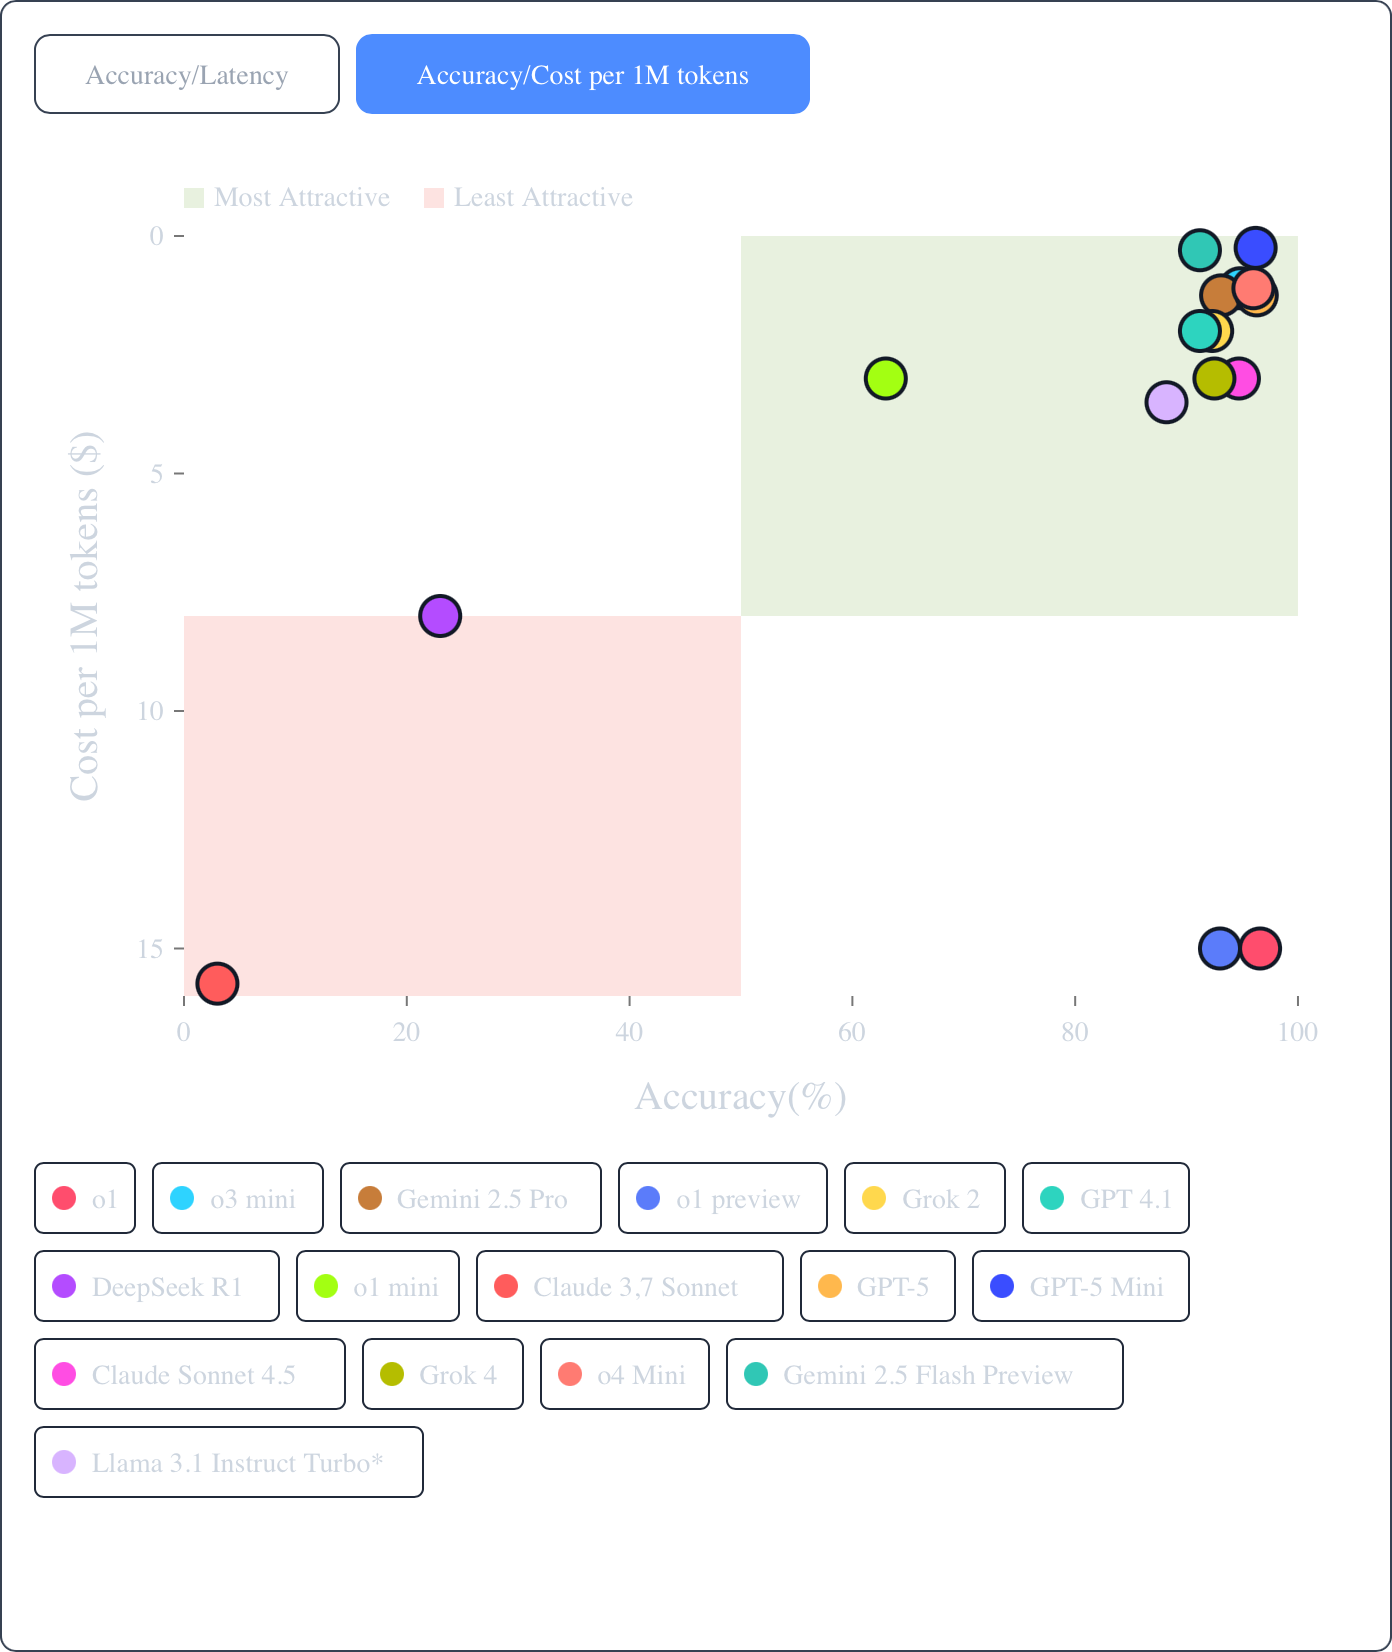
\includegraphics[width=0.88\textwidth]{SupplementaryImages/aiMultiple.png}
  \caption{Accuracy versus cost per million tokens for frontier LLMs in the
  AIMultiple healthcare benchmark survey \citep{dilmegani2025aimultiple}.}
  \label{fig:aimultiple_cost_accuracy}
\end{figure}

Against this evidence, \texttt{o4-mini-2025-04-16} was selected for
deployment.
It is an OpenAI reasoning model with multimodal input, combining staged
inference suited to multi-constraint narrative translation with a favourable
accuracy--cost trade-off for pre-study prompt iteration.
Ten baseline generations and one perturbation run met the Co-12 thresholds
in Section~\ref{sec:results_co12}.
Alternative chat and reasoning models remained viable, but \texttt{o4-mini}
offered the best balance of reasoning capability, multimodal support, and
deployment cost for this study.

% ── 2.6 ───────────────────────────────────────────────────────────────────────
\subsection{A Taxonomy for Explanation Artefact Quality: the Co-12 Framework}
\label{sec:prelim_co12}

Once an LLM is selected, the quality of its narrative outputs must still be
assessed systematically before they reach clinicians.
\citet{nauta2023anecdotal} propose a framework for evaluating explanation
artefacts themselves -- apart from model benchmarking
(Section~\ref{sec:prelim_llm_selection}) and from end-user comprehension
measures introduced in Section~\ref{sec:prelim_measurement}.
Their systematic review of XAI evaluation methods identifies twelve properties,
grouped into three categories.
\emph{Content} properties concern faithfulness to the underlying model:
Correctness, Completeness, Consistency, Continuity, Contrastivity,
and Covariate complexity.
\emph{Presentation} properties concern how the explanation is communicated:
Compactness, Composition, and Confidence.
\emph{User} properties concern fit with the recipient's needs and reasoning:
Context, Coherence, and Controllability.
Unlike the SCS or behavioural alignment tasks discussed below, Co-12 evaluates the
explanation text or visualisation as a designed artefact and can therefore be applied
during iterative design without requiring a user study.
In this paper, Co-12 provides the structured quality criterion against which successive
versions of the LLM prompt layer are evaluated
(Sections~\ref{sec:llm_design} and~\ref{sec:method_co12}).

% ── 2.7 ───────────────────────────────────────────────────────────────────────
\subsection{Measuring Interpretation Quality in XAI}
\label{sec:prelim_measurement}

Co-12, together with earlier technical metrics such as
\emph{fidelity} (how accurately the explanation reflects the model's
true decision process), \emph{stability} (whether similar inputs
produce consistent explanations), and \emph{sparsity} (whether
the explanation is concise, involving as few features as possible)
\citep{doshivelez2017rigorous, budhkar2025survey}, evaluates properties
of the explanation artefact itself. What these artefact-level criteria
cannot answer is whether a human actually understood the explanation
correctly or acted on it appropriately. \citet{suh2025fewer} quantify the scale of this problem in a large-scale
analysis of 18,254 XAI papers: only 128 papers (0.7\%) conducted any form
of human study to validate their explainability claims. This is not a
matter of underpowered studies or insufficient sample sizes -- the
overwhelming majority of papers present no human evidence whatsoever,
relying instead on technical metrics or anecdotal demonstration.
Calling a method ``explainable'' and showing that a human actually
understood it are therefore two very different things, and the XAI field
has largely confused them as the same thing.

Moving beyond technical metrics requires choosing a human-centered
evaluation instrument. Three approaches are available in the
literature, each operating at a different level and answering a
different question.

The System Causability Scale (SCS) by \citet{holzinger2020measuring}
is a 10-item Likert instrument modelled on the System Usability Scale.
It asks: \emph{was the explanation interface easy to use and did it
support causal understanding?} Items cover clarity, completeness,
timeliness, and whether the explanation supported decision-making.
The SCS is quick to administer and validated for medical AI contexts,
making it practical for clinical evaluation studies. Its limitation
is that it measures the user's experience of the explanation
rather than whether they understood the model correctly. A clinician
could rate an explanation as clear and complete while still holding
a wrong mental model of what the model does.

The in-context explanation quality framework by
\citet{kim2024human} operates at the level of the explanation
content. Derived from a systematic review of 73 papers across
multiple domains including healthcare, it proposes 11 properties:
understanding, ease of understanding, ease of use, satisfaction,
usefulness, trust, typicality, sufficiency, correctness, compactness,
and actionability. Compared to the SCS, it is broader in scope --
covering not just usability but also whether the explanation is
trustworthy, sufficient, and actionable. Two properties are
particularly notable: actionability (does the explanation
help the user determine what action to take?) and
correctness (does the user believe the explanation is
accurate?). These go beyond what the SCS captures. The key limitation
is the same as the SCS: all 11 properties are self-reported.
An explanation can score high on perceived correctness while the
user has drawn the wrong conclusion from it.

The third approach moves to behavioural measurement of mental
model shift. Rather than asking clinicians how they felt about an
explanation, \citet{jung2025evaluating} ask them directly which
features they believe drive a model prediction -- both before and
after seeing the explanation -- and then compare those beliefs to
the model's actual feature importance ranking. This produces an
objective alignment score: in their ICU length-of-stay study with
15 clinicians, the Spearman correlation between clinicians' feature
rankings and the model's rankings shifted from $-0.147$ before the explanation 
to $0.868$ after the explanation. Crucially, this behavioural measure can distinguish
beneficial alignment (where the clinician's understanding
genuinely moved toward what the model does) from automation
bias (where the clinician simply deferred to the model without
understanding why). This makes it the most direct measure of
interpretation quality, but it is also the most demanding: it
requires designing appropriate pre- and post-explanation tasks,
ensuring questions are sensitive enough to detect misinterpretation,
and coding responses against a ground-truth feature ranking.

The three approaches form a progression: the SCS measures perceived
usability and whether an explanation felt causally meaningful; Kim et
al.\ capture broader perceived quality, including correctness and
actionability; and behavioural tasks test whether a participant's actual
mental model shifted in the right direction. No single instrument fully
addresses the specific risk in this study: that clinicians will misinterpret
a correlational model as a causal one when its outputs are presented in
explanation form.

This gap motivates a purpose-built instrument, the \emph{Causal Attribution
Scale} (CAS), whose design draws on all three approaches. From the SCS it
takes the goal of measuring causal understanding, but treats that
understanding as something to be verified rather than self-reported. From
Kim et al.\ it takes correctness and actionability as the specific
constructs to measure -- the two properties most directly affected when
a clinician misreads a correlational model as causal. From the behavioural tradition of \citet{jung2025evaluating}
it adopts direct belief probes rather than quality ratings, so that a
clinician who found the explanation ``clear and useful'' but drew the wrong
causal conclusion is still detected. How these outcomes were analysed
is described in Section~\ref{sec:method_analysis}. Stepwise risk judgements and
open-text responses complement the CAS as further behavioural traces;
the between-subjects design (Groups A vs.\ B) tests whether the LLM
explanation layer changes these outcomes relative to KAN visualisations alone.

% ── 2.8 Synthesis ─────────────────────────────────────────────────────────────
\subsection{Synthesis}
\label{sec:prelim_synthesis}

Across these seven bodies of literature, a consistent pattern emerges: XAI in clinical
contexts succeeds when it supports the clinician's task (sense-making,
verification, safe action planning) and fails when it presents technically
accurate artefacts that do not map to clinical reasoning conventions or workflow
constraints \citep{tonekaboni2019clinicians, bienefeld2023solving,
anjara2023examining}. The LLM translation hypothesis is empirically reasonable:
narrative reframing of technical outputs can improve comprehension and
advice-taking compared to technical displays alone \citep{dams2025tell,
comparison2025shap}. However, the same evidence base introduces a critical
methodological constraint: improved acceptance is not the same as improved
interpretation correctness \citep{bansal2021does, bucinca2021trust}, and
conversational LLM interfaces specifically can amplify over-reliance by
creating an illusion of explanatory depth \citep{he2025conversational}.
Additionally, LLM narration introduces the failure modes of hallucination
and causal overreach \citep{omar2025hallucination, karimi2021algorithmic}.

This paper is positioned precisely at the intersection of these risks and
opportunities.
For the translation layer, \texttt{o4-mini-2025-04-16} was selected as a
cost-efficient reasoning model suited to multimodal, multi-constraint narrative
synthesis (Section~\ref{sec:prelim_llm_selection}).
The study tests whether this LLM intermediary improves clinicians'
interpretation of KAN-based in-hospital mortality predictions, using a
between-subjects design (Group~A: KAN visualisations; Group~B: KAN plus
a grounded LLM-generated explanation).
Outcomes include the five-item CAS, stepwise mortality-risk
judgements, and open-text clinical reasoning -- together operationalising
the distinction between perceived understandability, causal misinterpretation,
and reliance that the evaluation literature identifies as the key unresolved
gap.

% ══════════════════════════════════════════════════════════════════════════════
\section{Method}
\label{sec:method}
% ══════════════════════════════════════════════════════════════════════════════

This section describes how the study was designed and implemented.
It specifies the between-subjects protocol, participant criteria, and
three-step evaluation flow.
It then documents the MIMIC-based KAN model, the borderline-risk patient
case, and the Dutch study interface through which explanations are delivered.
Finally, it defines the instruments used to measure explanation artefact
quality (Co-12) and clinician interpretation (CAS, stepwise risk judgements,
and open-text responses).

% ── 3.1 ──────────────────────────────────────────────────────────────────────
\subsection{Study Design and Participants}
\label{sec:study_design}

This study employs a between-subjects design with two conditions.
Group~A participants review a KAN-based mortality-risk explanation
consisting of visualisations only; Group~B participants review the same
visualisations accompanied by an LLM-generated narrative explanation.
All participants evaluate the same borderline-risk patient case
presented in three sequential steps (described in
Section~\ref{sec:edge_patient}).

Participants were recruited through convenience sampling.
An ICU specialist distributed the study link within their professional
network, and additional candidates were solicited via LinkedIn or other professional networks.
Eligible participants hold a clinical role in an ICU setting
(intensivists or related ICU roles) and have sufficient familiarity
with laboratory and vital-sign values to interpret a patient
case. 
Group assignment is handled automatically by the study interface using
adaptive allocation: each new participant is directed to whichever group
has the smaller current response count, with ties assigned to Group~A.
This ensures balanced group sizes without requiring pre-stratification
or separate recruitment links.

The study follows a three-step sequential design, illustrated in
Figure~\ref{fig:study_design}.
In \textbf{Step~1} (blind assessment), participants receive only the
patient profile with no model output, and are asked to provide a baseline
mortality risk estimate, their clinical reasoning, and proposed
interventions.
In \textbf{Step~2}, the KAN model's predicted mortality probability is
revealed. Participants record a revised risk estimate and indicate whether
the model score changed their view.
Recording this intermediate estimate is essential: without it, any shift
in the final judgment could not be disentangled from the mere exposure to
the model's numeric prediction. If participants are already anchored to
that number before seeing the explanation, attributing the shift solely
to the explanation would inflate its apparent effect. Comparing the
Step~1 and Step~2 estimates therefore allows anchoring to be quantified
independently (measurement~i).
In \textbf{Step~3}, participants in Group~A receive the feature-level
spline charts only, while those in Group~B additionally receive an
LLM-generated narrative explanation. Both groups then provide a final risk
estimate, complete the Causal Attribution Scale (CAS), and give open-text
clinical reasoning. Beyond the risk estimate, the CAS captures whether
participants incorrectly assign causal meaning to the model's
correlational output, and the open-text responses reveal the clinical
concepts that participants draw on when reasoning about the case.
Comparing the final estimates, CAS scores, and open-text responses
between the two groups isolates the incremental effect of the narrative
explanation over the charts alone (measurement~ii). The instruments used
to assess interpretation quality are described in
Section~\ref{sec:method_prompts}.

\begin{figure}[h]
  \centering
  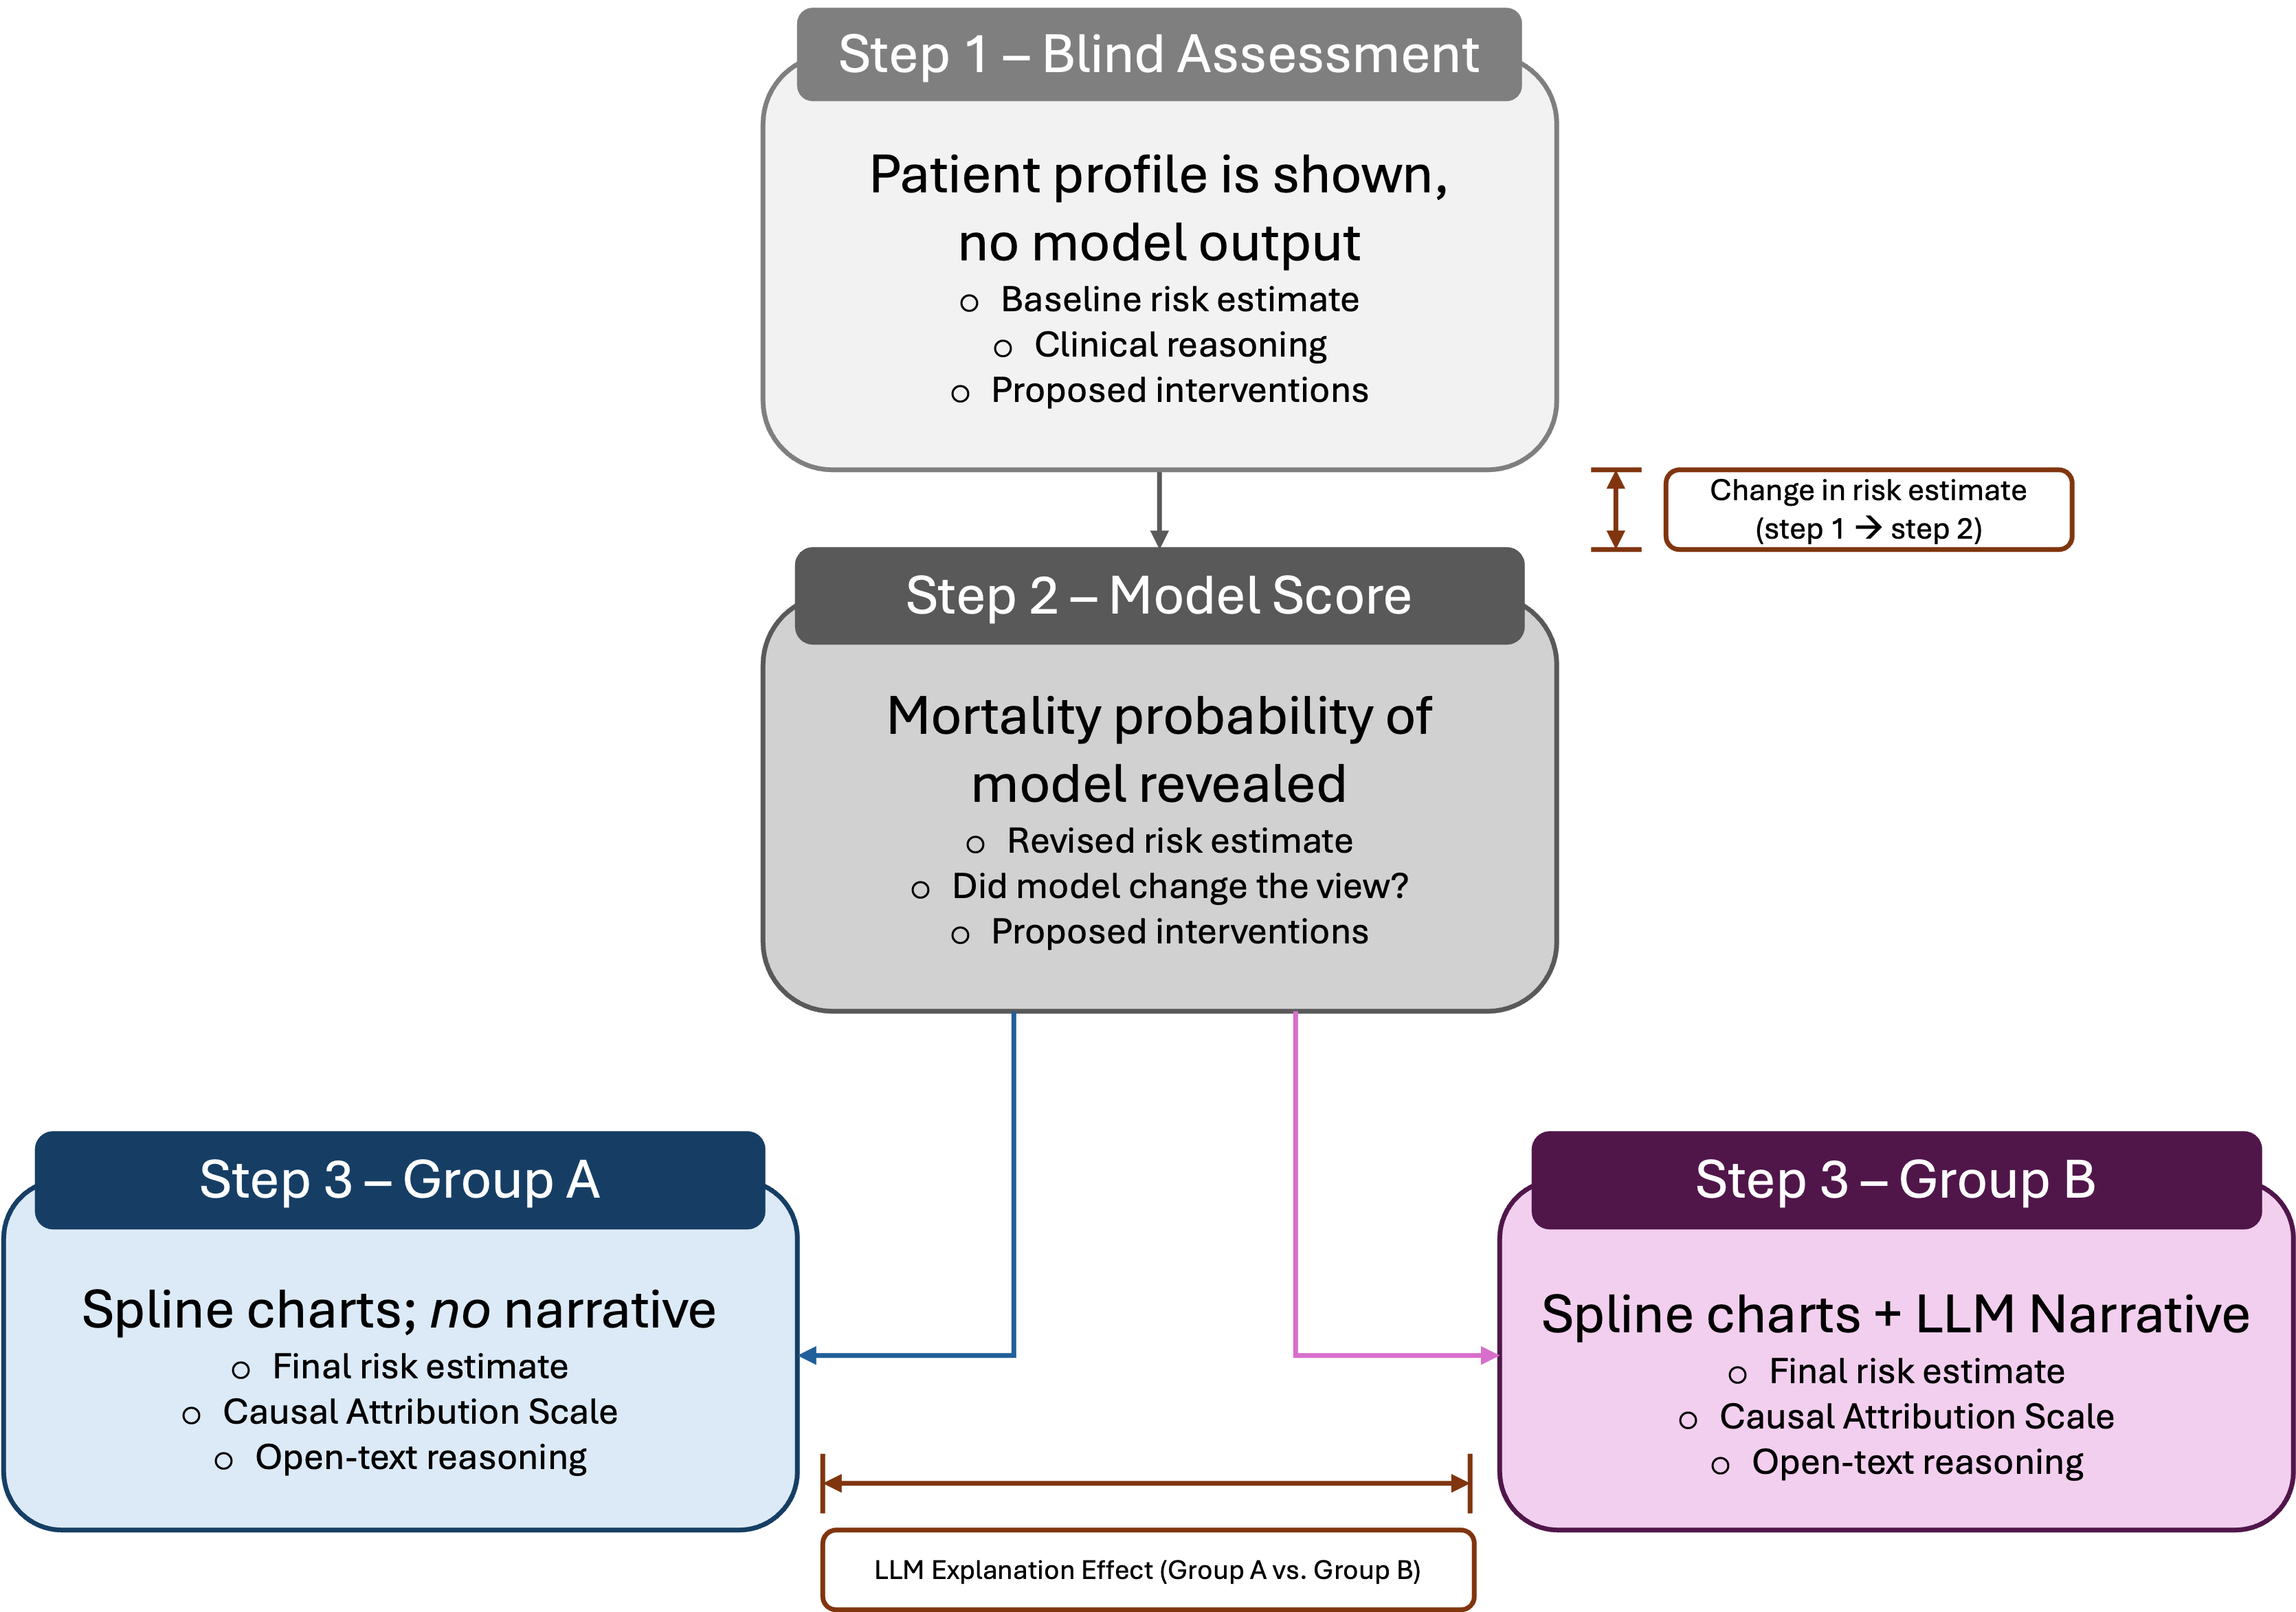
\includegraphics[width=0.82\textwidth]{SupplementaryImages/studyDesign.png}
  \caption{Three-step between-subjects study design.}
  \label{fig:study_design}
\end{figure}

Participant responses were collected anonymously; no personally
identifiable information was recorded and no signed consent was required.
The patient case presented in the study interface is drawn from the
MIMIC-IV v2.2 database \citep{johnson2023mimic}; its selection and the
cohort criteria used to train the underlying model are described in
Section~\ref{sec:edge_patient}. Access to MIMIC-IV was obtained through
completion of the CITI \emph{Data or Specimens Only Research} training course.

% ── 3.2 [placeholder] ────────────────────────────────────────────────────────
\subsection{Study Interface and Materials}
\label{sec:edge_patient}
\subsubsection{Dataset}

The data were drawn from MIMIC-IV v2.2 \citep{johnson2023mimic}, a
restricted-access database of ICU admissions at Beth Israel Deaconess
Medical Center (2008--2019). Access was obtained under a PhysioNet
credentialed data use agreement. Model training used a preprocessed MIMIC-IV extract based on the cohort
construction of \citet{zhang2023}: adult ICU patients meeting Sepsis-3
criteria (suspected infection with SOFA $\geq 2$), age $\geq 18$ years,
and a qualifying \texttt{icustays} record of at least 24 hours, with
one such stay per patient and all input features aggregated from the
first 24 hours of that stay. The original extract contains 14{,}620 ICU
stays; the prediction target was relabelled from sepsis-associated
delirium to in-hospital mortality for this study. This dataset was used
because the sepsis ICU population and 24-hour feature window matched the
study aim, the vitals, laboratory values and severity scores were already
curated and quality-checked, and early physiology is captured before
longer treatment effects dominate. After feature selection and
preprocessing, 11{,}197 stays remained and were split 70/30 into
training and test sets using stratified sampling (random seed 42),
resulting in 7{,}838 training and 3{,}359 test stays.

\subsubsection{Feature Selection and Preprocessing}

The 29 input features span four groups: demographics (age, weight, sex),
vital signs (temperature, heart rate, respiratory rate,
SpO\textsubscript{2}, SBP, DBP, MBP), laboratory values (WBC,
haemoglobin, platelets, BUN, creatinine, glucose, sodium, chloride,
potassium, magnesium, calcium, phosphate, INR, PT, PTT, bicarbonate,
anion gap), and clinical severity scores (GCS, SOFA). Active
interventions (mechanical ventilation, vasopressors, CRRT, sedation),
comorbidities, race, and ICU department type were excluded to reduce
confounding and to retain a feature set that is interpretable in
isolation. Continuous features were Min-Max normalised to $[0, 1]$;
the binary sex feature was label-encoded; GCS and SOFA were normalised
as ordinal variables. Missing values were imputed using the column
median prior to normalisation.

\subsubsection{KAN Model}

The predictive model is a Kolmogorov--Arnold Network \citep{liu2024kan}
trained to predict in-hospital mortality from data collected in the first
24 hours of ICU admission. KANs replace the fixed scalar weights of a
conventional neural network with learnable univariate spline functions on
each edge, making the model's internal computations directly visualisable
as a set of input--output curves.

The network has the shape $[29 \to 3 \to 2]$: 29 input features, a single
hidden layer of 3 nodes, and a 2-class softmax output (survived / died), as
shown in Figure~\ref{fig:kan_arch}. Each spline uses cubic B-splines ($k =
3$) with a grid of 3 intervals, yielding 1{,}116 trainable parameters in
total. Hyperparameters were selected by a grid search over hidden nodes
(1--5), epochs (5, 10, 20), and L-BFGS learning rate (0.0001--1.0); full
results are reported in Table~\ref{tab:sweep}. AUROC varied only narrowly
across all 74 valid configurations (70.6--74.5\%), and no configuration
strictly dominated the chosen setting on both AUROC and FPR. The
$[29\to3\to2]$ architecture with 5 epochs at the default learning rate
(AUROC = 74.5\%) was selected: 3 hidden nodes keep the network directly
visualisable as a set of learnt spline curves, and the configuration is not
outperformed by any more complex alternative on the relevant metrics. The
model was trained with light L1 regularisation ($\lambda = 0.0001$) and
class-weighted cross-entropy loss (survived $1\times$, died $6\times$)
rather than resampling, to avoid distorting the natural feature
distributions.

\begin{figure}[htbp]
  \centering
  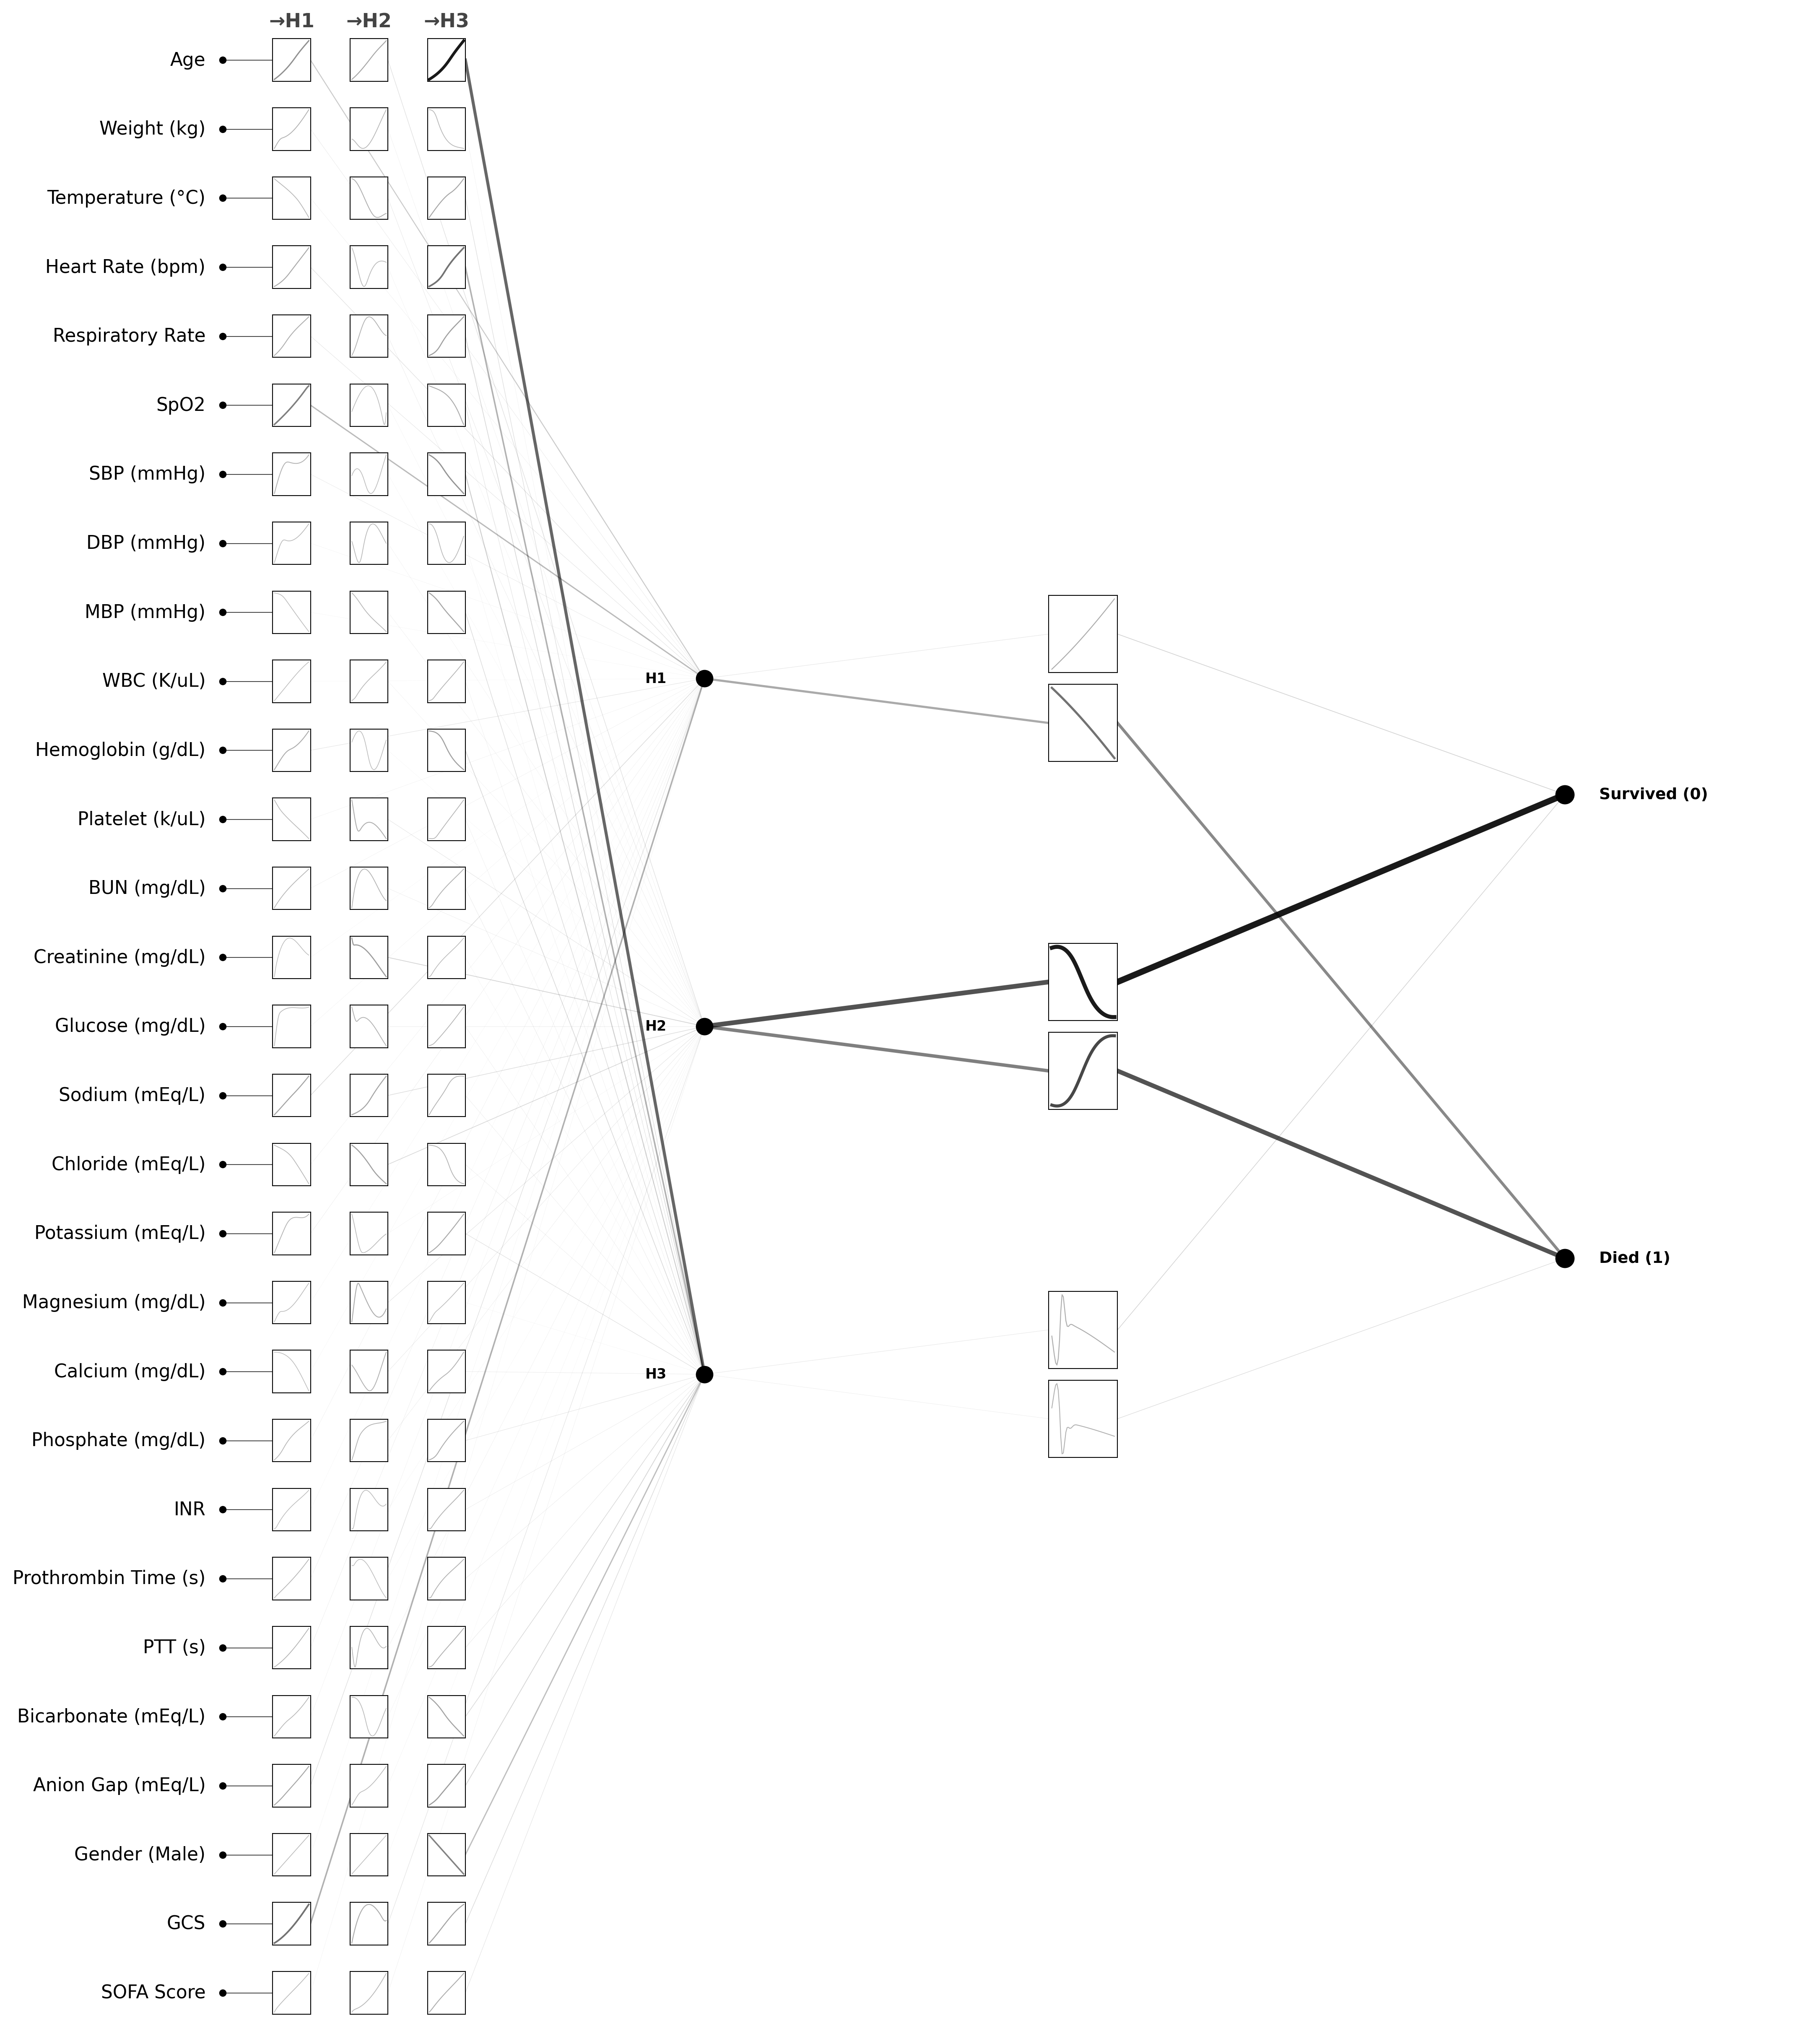
\includegraphics[width=0.72\textwidth]{../hospMort/scripts/results/plots/kan_hosp_mort_annotated.png}
  \caption{Trained KAN architecture ($[29 \to 3 \to 2]$); edge width reflects mean absolute spline activation across the test set.}
  \label{fig:kan_arch}
\end{figure}

A classification threshold of 0.5383 was selected by an FPR-constrained
criterion: the highest threshold on the ROC curve
(Figure~\ref{fig:kan_roc}) that keeps the false-positive rate at or below
25\%. Without this constraint the same model flags 30.6\% of survivors as
high-risk at the default threshold; applying the cap tightens this to
25.0\% while maintaining AUROC. The 25\% ceiling was chosen to keep
positive predictions selective enough to be clinically credible: a model
that flags one in three survivors as high-risk produces risk scores that
are too diffuse to carry meaningful signal for study participants or
clinicians. In a clinical deployment setting the threshold would instead be
set by clinical stakeholders based on an explicit acceptable miss rate.

\begin{figure}[htbp]
  \centering
  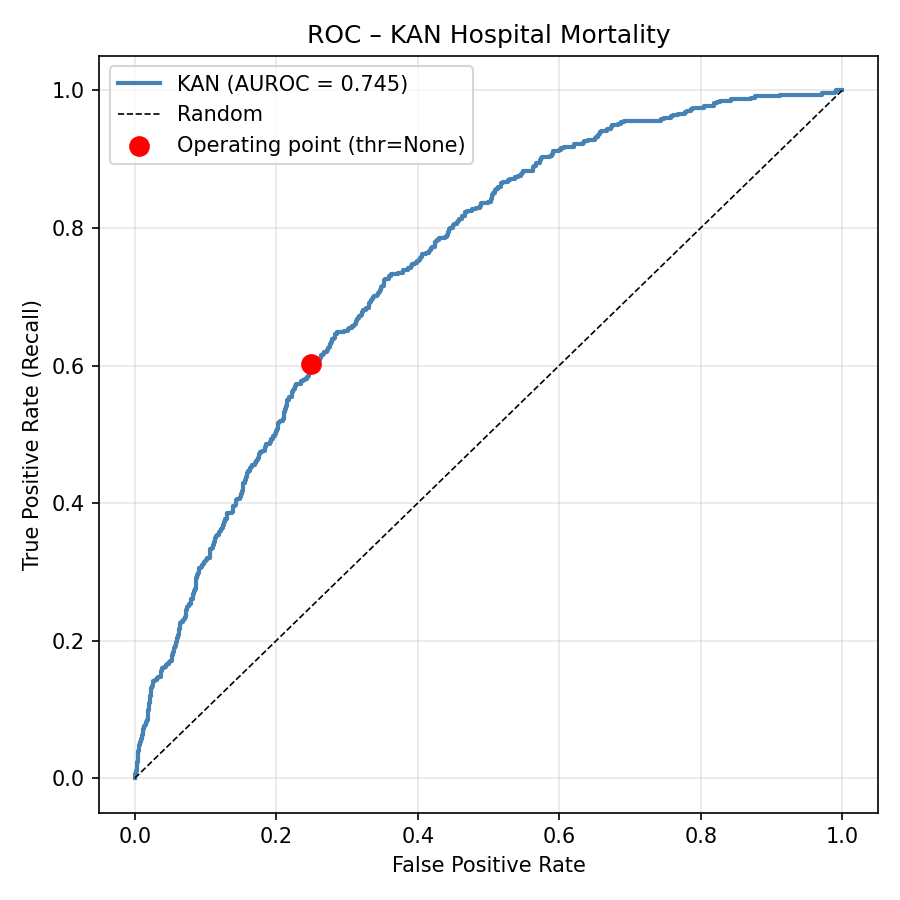
\includegraphics[width=0.60\textwidth]{../hospMort/scripts/results/plots/roc_curve.png}
  \caption{ROC curve on the test set (AUROC = 0.745). The red dot marks the FPR-constrained operating point (FPR = 25\%, recall = 60\%).}
  \label{fig:kan_roc}
\end{figure}

Full test-set performance is reported in Table~\ref{tab:kan_metrics}. The
low precision for the died class (28.4\%) is the direct consequence of the
FPR ceiling: roughly three out of four patients flagged as high-risk had in
fact survived. This trade-off was acceptable for the study purpose, where participants
evaluated a single patient case rather than operating a real triage screen.

\begin{table}[H]
  \centering
  \caption{KAN model performance at the FPR-constrained threshold (0.5383).}
  \label{tab:kan_metrics}
  \begin{tabular}{lrrrr}
    \toprule
    & Precision & Recall & F1 & Support \\
    \midrule
    Survived (0) & 0.92 & 0.75 & 0.83 & 2{,}884 \\
    Died (1)     & 0.28 & 0.60 & 0.39 &     475 \\
    \addlinespace
    Macro avg    & 0.60 & 0.68 & 0.61 & 3{,}359 \\
    \midrule
    \multicolumn{5}{l}{\small AUROC = 0.745\quad Accuracy = 72.9\%\quad FPR = 25.0\%\quad FNR = 39.8\%} \\
    \multicolumn{5}{l}{\small TP = 286\quad FP = 720\quad FN = 189\quad TN = 2{,}164} \\
    \bottomrule
  \end{tabular}
\end{table}

\subsubsection{Patient Case}

To select a suitable study case, an experienced ICU specialist was consulted.
The goal was to identify a genuine \emph{edge case}: a patient whose
predicted mortality probability sits in a range that a clinician would
naturally experience as uncertain -- where the question of whether the
patient will survive is not immediately obvious from the clinical
picture, and the probability itself prompts reflection rather than
simply confirming a predictable conclusion. The clinician advised that this
required combining a borderline KAN probability (roughly 60--70\%) with
an outcome of actual in-hospital death and a presentation free of
immediately alarming markers (e.g.\ extreme organ failure scores or
haemodynamic instability) that would pre-anchor clinical judgement.

To support the selection process, a patient calculator tool was developed
(Appendix~\ref{app:patient_calc}) that allows a user to specify a
clinical profile and retrieves the nearest matching patient from the test
set by Euclidean distance on normalised features. The tool also displayed
a set of pre-selected candidates meeting the above criteria
(Appendix~\ref{app:candidates}): KAN probability between 60\% and 70\%,
actually deceased, and no single feature value that is unambiguously
alarming in isolation.

The clinician approved \textbf{patient \#8259} (male, 68 years; KAN
P(died) = 60.2\%; indexed ICU stay \texttt{35676599}, 76~hours). Within
the same hospital admission the patient was managed on ward and oncology
units before this qualifying ICU stay, with an earlier brief MICU
episode recorded only as intra-hospital transfers rather than as a separate
\texttt{icustays} row (Appendix~\ref{app:bigquery}, Query~3). The patient has a SOFA score of 2 and GCS of 14,
indicating mild organ dysfunction and near-normal consciousness, making
the case superficially reassuring. The clinically notable finding is a
markedly elevated aPTT of 91.6\,s (approximately three times the normal
upper limit), suggesting a coagulation abnormality that is easily
overlooked without close inspection of the lab panel. This combination
-- a borderline predicted risk with one subtle but clinically
significant laboratory finding -- was judged to make patient \#8259 a
strong vehicle for studying how model explanations influence reasoning.

Because the preprocessed MIMIC-IV CSV used for model training contains
only the 24-hour aggregate features and no timestamps, additional data
were retrieved directly from the raw MIMIC-IV database via BigQuery to
give study participants sufficient clinical context for a realistic
judgement. Queries were run against MIMIC-IV v3.1 on PhysioNet using
\texttt{stay\_id} 35676599 and \texttt{hadm\_id} 25820763, retrieving:
hospital admission details (admission time, type, location, and
discharge destination); the ICU stay timeline; ICD-10 discharge
diagnoses; timestamped vital signs and laboratory values from the first
24 hours of ICU admission; SOFA subscores at the time of the lab draw;
and medications administered prior to that timepoint
(Appendix~\ref{app:bigquery}). This richer
context -- showing not just the feature values but \emph{when} they
were measured relative to admission and what treatments were already
under way -- was used to construct the clinical profile shown to
participants in the study interface.

\subsubsection{Study Interface}
\label{sec:study_interface}

The study was administered through a custom web-based interface built with
Flask~(Python) and hosted on Railway. All screens are reproduced in
Appendix~\ref{app:interface}
together with their full English translations. Participants first read a
welcome page explaining the study purpose and confirming anonymity and
voluntary participation, then stated their professional role before
entering the three-step patient case.

\paragraph*{Step 1 -- Blind assessment (Figure~\ref{fig:screen1}).}
The patient profile (header, clinical context narrative, vital signs, and
laboratory values) was shown without any model output.
Because the underlying model was trained on MIMIC-IV data stored in
US-customary units (e.g.\ haemoglobin in g/dL, creatinine in mg/dL,
glucose in mg/dL), all laboratory values displayed to participants were
converted to SI units standard in Dutch clinical practice: haemoglobin
to mmol/L, creatinine and BUN to \textmu{}mol/L and mmol/L respectively,
glucose to mmol/L, and electrolytes and coagulation values left in
their native mEq/L or seconds, which coincide with European SI reporting.
Participants were asked: \emph{``What is your initial assessment of the
risk that this patient will die during this admission?''} (low / moderate /
high / uncertain), with two free-text fields for clinical reasoning and
proposed interventions.

\paragraph*{Step 2 -- Model output revealed (Figure~\ref{fig:screen2}).}
The KAN model's predicted in-hospital mortality probability (60.2\%,
elevated) was displayed. Participants revised their risk estimate and
answered: \emph{``Has the model output changed your further assessment?
Why (not)?''}

\paragraph*{Step 3 -- Model explanation
(Figures~\ref{fig:screen3a1}--\ref{fig:screen3b2}).}
\citet{liao2020questioning}'s question taxonomy
(Section~\ref{sec:prelim_clinician}) distinguishes several explanation
needs, but prior work shows that multiplying separate XAI views for each
need compounds cognitive burden and accessibility failures: explanations
exist yet remain too technical to use or misaligned with clinical mental
models \citep{bienefeld2023solving, tonekaboni2019clinicians}.
Because the between-subjects comparison concerns the LLM narrative layer
rather than an exhaustive audit of every taxonomy category, the interface
was not designed to present a dedicated visualisation for each explanation
question. Instead, both groups received one
consolidated twelve-panel chart of spline-based feature contributions
annotated with the patient's own values: the six features with the largest
positive contributions and the six with the largest negative contributions
for this patient, selected from the physiological features only. Each panel
shows the learned contribution curve for one measurement, with the patient's
current value marked; together, the grid combines the \emph{Why?}, a
partial \emph{Why not?} (why a different value along that feature's curve
would have pushed the isolated signal the other way), and an implicit
\emph{How to be that?} reading by showing where the curve would place the
model signal at other values. These readings explain how the bedside model
formed its prediction -- to support understanding and warranted trust in such
models, not to direct clinical action -- and are always presented as an
isolated-panel view, not as a full interactive counterfactual over the joint
model.
How each feature's per-hidden-edge splines are aggregated into the single
curve shown in the interface is illustrated in Figure~\ref{fig:kan_sum}.

\begin{figure}[H]
  \centering
  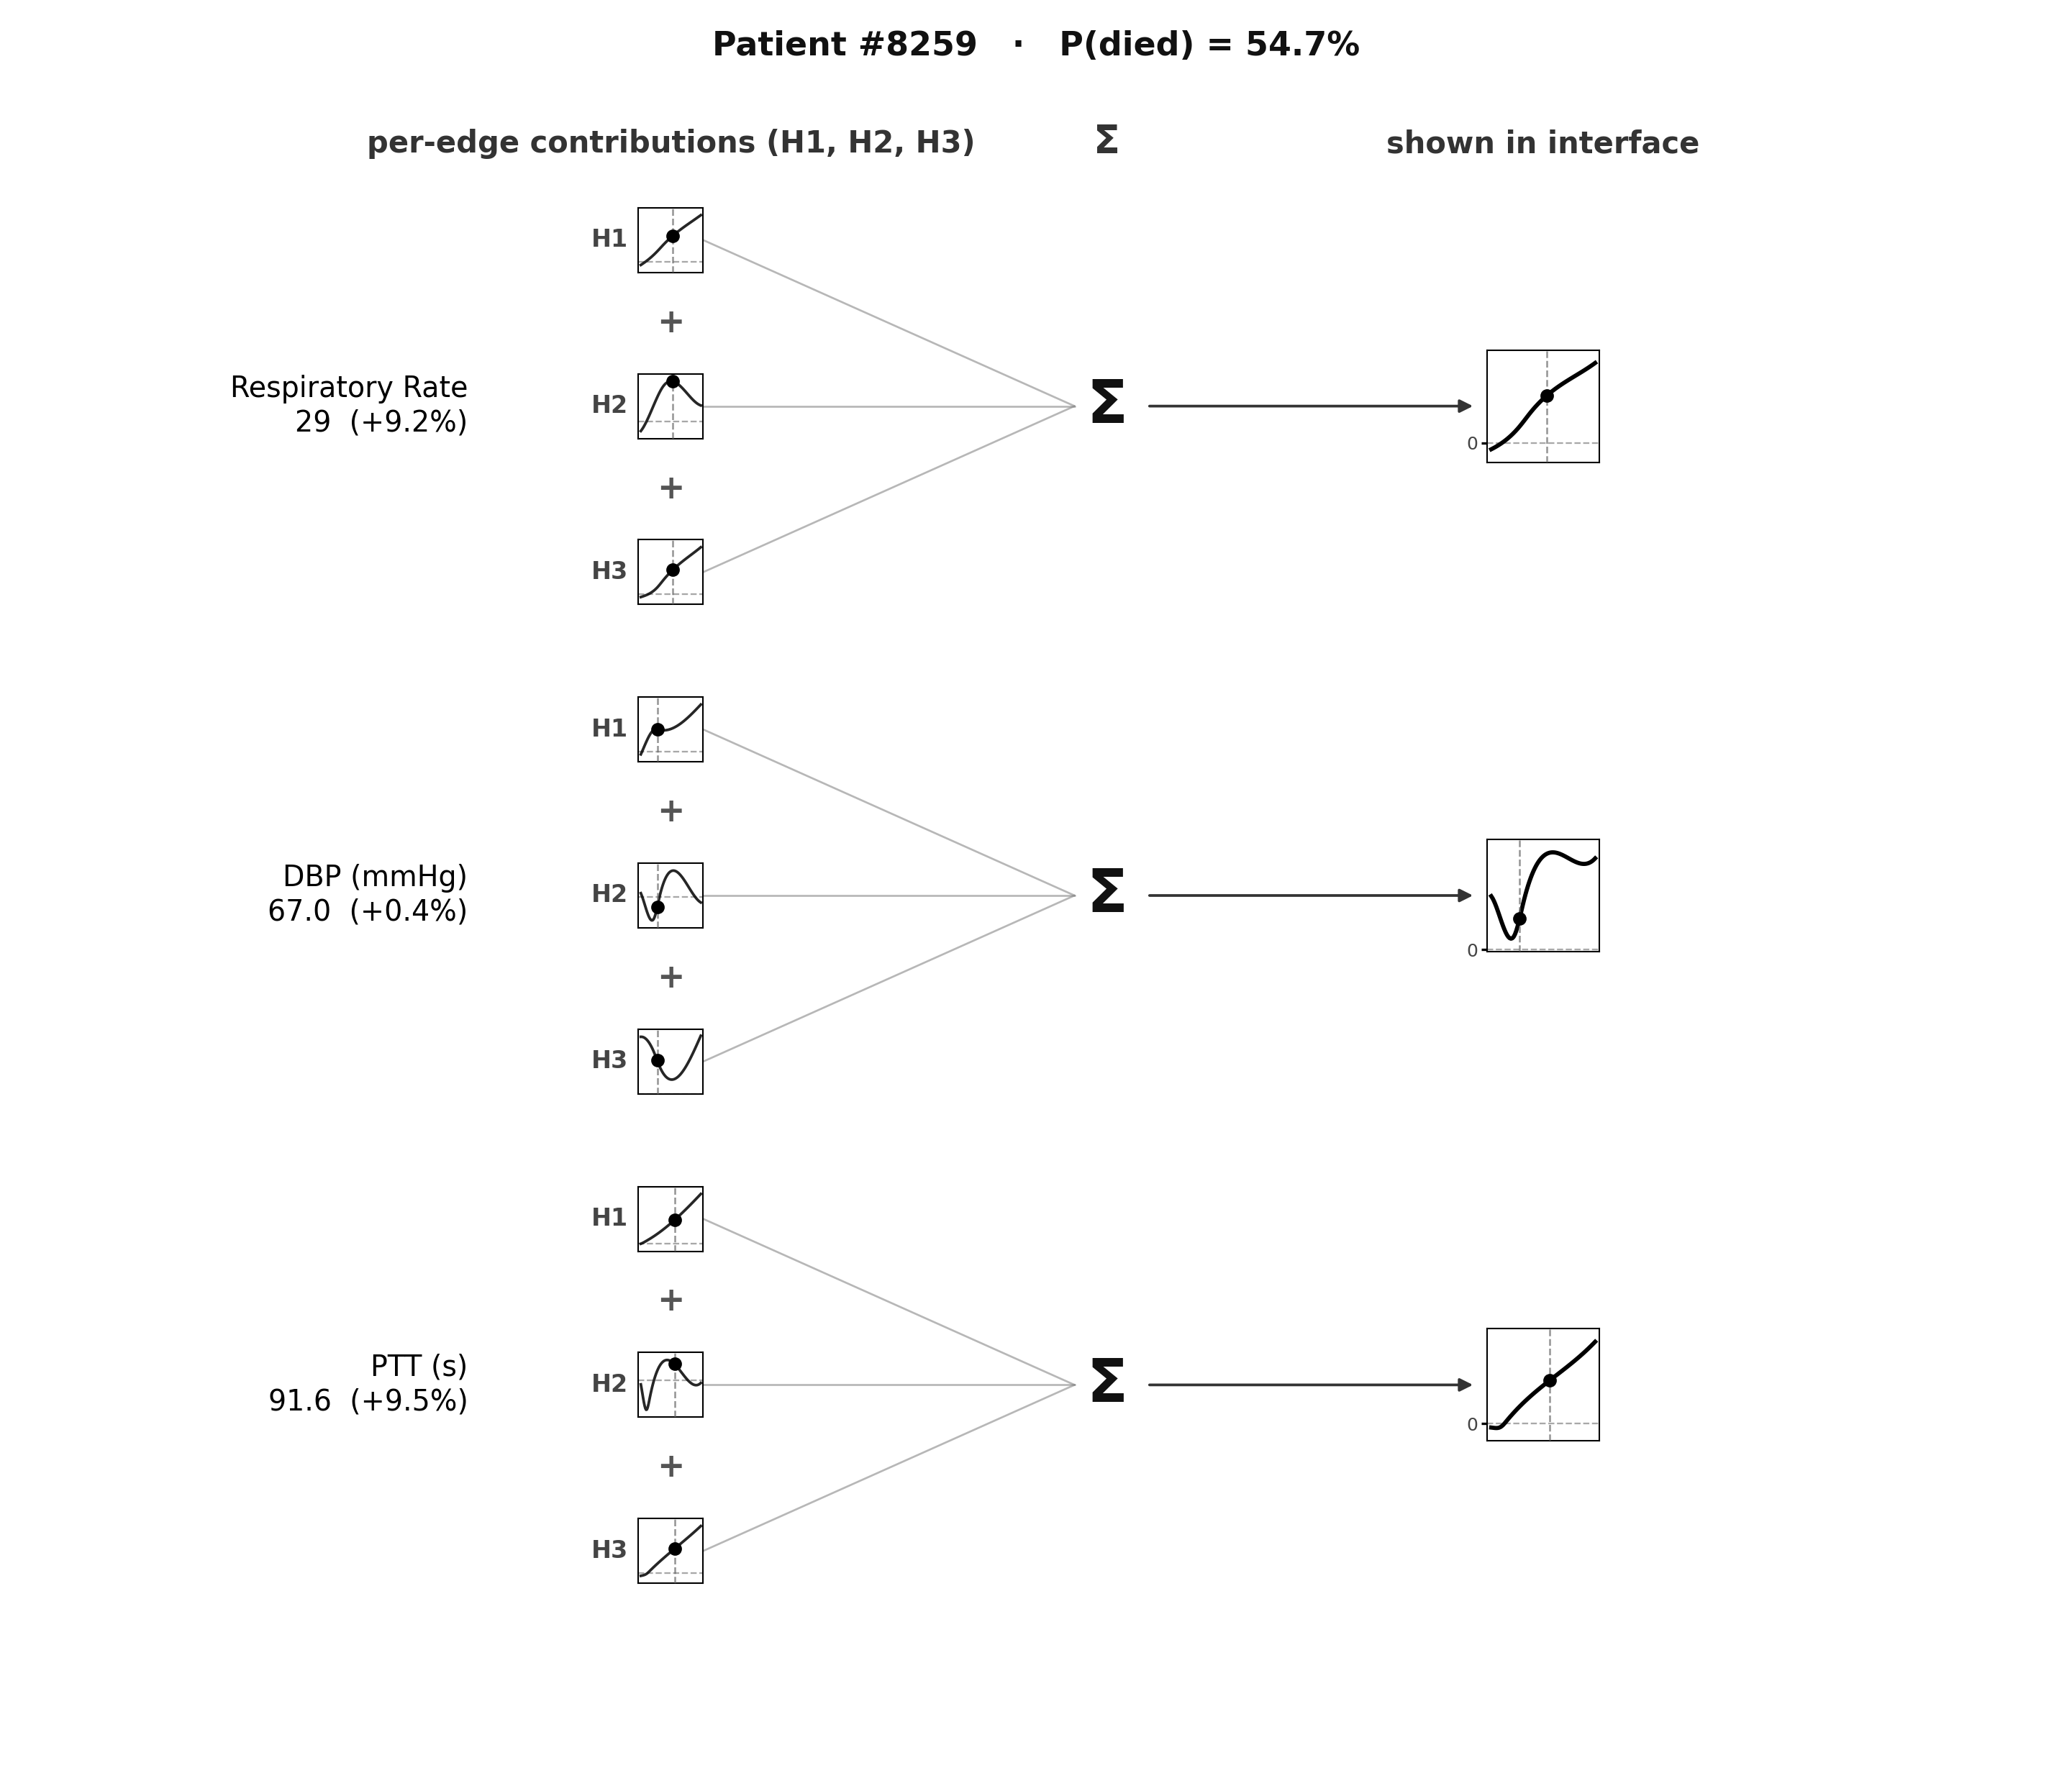
\includegraphics[width=0.72\textwidth]{../hospMort/scripts/results/plots/kan_sum_to_interface.png}
  \caption{For three example features, the three per-hidden-edge splines
    (H1, H2, H3) are summed ($\Sigma$) to produce the single
    feature-contribution curve displayed in the study interface.}
  \label{fig:kan_sum}
\end{figure}

Age and
sex were deliberately excluded from the displayed panel even where their
model contributions were non-negligible. Clinicians already incorporate
patient demographics into their clinical reasoning independent of any
model; presenting demographic contributions alongside physiological ones
would conflate the model's learned physiological associations with
pre-existing demographic knowledge, making it difficult to isolate the
extent to which the physiological explanation shapes clinical judgement.
The panel was therefore restricted to the twelve highest-contributing
physiological features. Group~B additionally received an LLM-generated narrative explanation
below the charts; the design and prompt engineering of this narrative are
described in Section~\ref{sec:llm_design}. Participants then gave
their definitive risk estimate, free-text reasoning, and answered:
\emph{``Has the model output influenced your definitive decision?''}, followed
by the five-item Causal Attribution Scale; interpretation quality was
measured as described in Section~\ref{sec:method_analysis}.

% ── 3.3 ──────────────────────────────────────────────────────────────────────
\subsection{Measuring Interpretation Quality}
\label{sec:method_prompts}

\subsubsection{LLM Explanation Design}
\label{sec:llm_design}

Group~B participants received a short Dutch narrative generated by
OpenAI \texttt{o4-mini} displayed directly below the twelve spline
charts (Figure~\ref{fig:screen3b1}). The narrative was generated once
per session at page load and remained fixed for the participant.

\paragraph*{Input structure.}
The model received a multimodal message consisting of a system prompt
and a user message containing both a PNG image and structured text;
the full prompt is reproduced in Appendix~\ref{app:llm_prompt}. The
image was the same twelve-panel spline chart shown to the participant.
The text payload contained the predicted mortality probability, one
structured line per panel with the patient's SI value, OLVG adult
reference range~\citep{olvg2024}, spline activation, and percentage
contribution, and a full signal table covering all model inputs
(excluding demographics and ICU subtype indicators) to prevent
hallucination on features outside the twelve panels.

\paragraph*{System-prompt constraints.}
The system prompt imposed the following constraints informed
iteratively by Co-12 criteria~\citep{nauta2023anecdotal}: professional Dutch
only with no markdown; no description of chart colours or percentage
labels; strictly correlational framing with no causal claims or
treatment advice; no machine-learning jargon; and a fixed
three-paragraph structure (9--12 sentences) introduced by a single
fixed heading, with no closing invitation to continue the conversation.

\paragraph*{Output structure.}
The required paragraphs were: (1)~two sentences on the predicted probability
and which measurements drove the signal upward versus downward;
(2)~five to six sentences on the correlational nature of the estimate and
the value of transparent model explanations for clinical trust calibration;
(3)~two to four sentences on the most striking pattern a clinician might find
surprising -- prioritising out-of-range values associated with lower predicted
risk, otherwise in-range values associated with higher risk -- with a cautious
qualifier, or -- if nothing was noteworthy -- a sentence on the
isolated-panel versus whole-model principle (nine to twelve sentences in
total). An example of the resulting narrative as shown to
participants is visible in Figure~\ref{fig:screen3b1}. The model was
\texttt{o4-mini-2025-04-16}: a reasoning model that does not accept a
\texttt{temperature} parameter; each call used \texttt{max\_completion\_tokens}
with a requested budget of 420 tokens (raised to an 8192-token floor required
by the reasoning API).

The output constraints were refined iteratively: each observed failure in the
LLM narrative was traced to a specific Co-12 criterion and addressed by a
targeted change to the prompt file or the application file.
Figure~\ref{fig:prompt_timeline} summarises the eleven most important problems
and their fixes.

% ── Prompt refinement timeline ───────────────────────────────────────────────
\begin{figure}[htbp]
\centering
\definecolor{tagCbg}{HTML}{EFF6FF}
\definecolor{tagCbd}{HTML}{BFDBFE}
\definecolor{tagCtx}{HTML}{1E40AF}
\definecolor{tagPbg}{HTML}{F0FDF4}
\definecolor{tagPbd}{HTML}{BBF7D0}
\definecolor{tagPtx}{HTML}{166534}
\definecolor{tagUbg}{HTML}{FEFCE8}
\definecolor{tagUbd}{HTML}{FDE68A}
\definecolor{tagUtx}{HTML}{92400E}
\definecolor{cardbg}{HTML}{F9FAFB}
\definecolor{cardbd}{HTML}{E8EDF2}
\definecolor{dotbg}{HTML}{334155}
\definecolor{spinecol}{HTML}{E2E8F0}
\definecolor{probtx}{HTML}{0F172A}
\definecolor{fixtx}{HTML}{475569}

\newcommand{\tagC}[1]{%
  \tikz[baseline=(t.base)]\node[fill=tagCbg,draw=tagCbd,rounded corners=2pt,
    inner xsep=3.5pt,inner ysep=1pt,
    font=\fontsize{6}{7}\selectfont\bfseries,text=tagCtx](t){#1};}
\newcommand{\tagP}[1]{%
  \tikz[baseline=(t.base)]\node[fill=tagPbg,draw=tagPbd,rounded corners=2pt,
    inner xsep=3.5pt,inner ysep=1pt,
    font=\fontsize{6}{7}\selectfont\bfseries,text=tagPtx](t){#1};}
\newcommand{\tagU}[1]{%
  \tikz[baseline=(t.base)]\node[fill=tagUbg,draw=tagUbd,rounded corners=2pt,
    inner xsep=3.5pt,inner ysep=1pt,
    font=\fontsize{6}{7}\selectfont\bfseries,text=tagUtx](t){#1};}
\newcommand{\tlnum}[1]{%
  \tikz[baseline=(t.base)]\node[circle,fill=dotbg,text=white,
    font=\fontsize{7}{7}\selectfont\bfseries,
    inner sep=0pt,minimum size=14pt](t){#1};}

\fontsize{8}{11}\selectfont
\setlength{\tabcolsep}{4pt}
\renewcommand{\arraystretch}{1.2}
\noindent
% header row
\begin{tabular}{@{}p{0.55cm}@{\hspace{2pt}}p{4.0cm}p{5.2cm}p{3.6cm}@{}}
\multicolumn{1}{@{}c@{\hspace{2pt}}}{} &
  \fontsize{7}{9}\selectfont\bfseries\color{probtx} Problem &
  \fontsize{7}{9}\selectfont\bfseries\color{probtx} Fix &
  \fontsize{7}{9}\selectfont\bfseries\color{probtx} Co-12 addressed \\[3pt]
%
\tlnum{1} &
  \textbf{LLM could hallucinate feature values} &
  Inject exact values per call; PNG matching UI; full-signal appendix; forbid appendix paste. &
  \tagC{Correctness}~\tagP{Confidence}\\[2pt]
\tlnum{2} &
  \textbf{Training statistics mixed with panel slope} &
  Separate training data from panel direction; \texttt{chart\_facts} for internal grounding only. &
  \tagC{Correctness}~\tagU{Coherence}\\[2pt]
\tlnum{3} &
  \textbf{Too much chart legend; too little patient context} &
  One heading; \S1 = probability + features pulling up/down; remove chart walkthrough. &
  \tagU{Context}~\tagP{Compactness}\\[2pt]
\tlnum{4} &
  \textbf{English mixed into Dutch prompt strings} &
  Full Dutch system prompt; Dutch labels in the application file; English only for API identifiers. &
  \tagP{Composition}~\tagU{Context}\\[2pt]
\tlnum{5} &
  \textbf{Prescriptive language ("u herkent\ldots", "een arts zou\ldots")} &
  Retrospective association only; hypotheticals as model probability only; no treatment steering. &
  \tagU{Context}~\tagU{Coherence}~\tagP{Confidence}\\[2pt]
\tlnum{6} &
  \textbf{False contrast: alarming K while higher predicted risk} &
  \textit{terwijl} only for true direction mismatches; \S3 optional ($\leq$1 example, no repeat from \S1). &
  \tagC{Correctness}~\tagC{Contrastivity}\\[2pt]
\tlnum{7} &
  \textbf{Two headings + synthesis boilerplate + chat invite} &
  One heading; no synthesis closer; chat removed from step-3 UI; single cached intro per session. &
  \tagP{Compactness}~\tagP{Composition}\\[2pt]
\tlnum{8} &
  \textbf{Demographics narrated in the explanation} &
  Age, Gender, Weight excluded from detail panels and LLM tables; model uses them internally only. &
  \tagU{Context}\\[2pt]
\tlnum{9} &
  \textbf{Prompt $\sim$630 lines; rigid rubric} &
  Reduced to $\sim$179 lines; deleted graph 1 \& 2 templates; lighter paragraph instructions. &
  \tagP{Compactness}~\tagC{Consistency}\\[2pt]
\tlnum{10} &
  \textbf{\S2 disclaimer only -- no positive XAI framing} &
  \S2 closes with one sentence on XAI value: ML transparency for clinical trust calibration. &
  \tagU{Context}~\tagP{Confidence}\\[2pt]
\tlnum{11} &
  \textbf{Reference-range mislabel (e.g.\ Mg 0.93\,mmol/L called below 0.70--0.99)} &
  Pre-computed \textit{binnen/onder/boven referentie}; \S3: one counter-intuitive pattern (in-range + higher risk, or out-of-range + lower risk); skip in-range protective. &
  \tagC{Correctness}~\tagU{Coherence}\\[4pt]
\multicolumn{4}{@{}l@{}}{%
  \fontsize{6.5}{9}\selectfont\color{fixtx}
  \tagC{Content} Correctness $\cdot$ Contrastivity $\cdot$ Consistency\quad
  \tagP{Presentation} Compactness $\cdot$ Composition $\cdot$ Confidence\quad
  \tagU{User} Context $\cdot$ Coherence}\\
\end{tabular}
\caption{Iterative refinement of the LLM prompt: observed problem, fix applied to
  the prompt file or the application file, and Co-12 criterion addressed~\citep{nauta2023anecdotal}.}
\label{fig:prompt_timeline}
\end{figure}

\subsubsection{Descriptive Analysis of Interpretation Outcomes}
\label{sec:method_analysis}

Given the small convenience sample, inferential hypothesis tests were
not conducted. Outcomes were summarised descriptively within and
between groups (Group~A: KAN charts only; Group~B: KAN charts + LLM
narrative), with individual responses quoted where they illustrated
typical or deviant interpretation patterns. The analysis followed the
three-step sequence in Figure~\ref{fig:study_design}: baseline judgement
(Step~1), response to the revealed model score (Step~2), and final
judgement after the explanation stream (Step~3), with the between-group
comparison isolating the incremental effect of the LLM narrative.
It examined whether the explanation stream changed interpretation in
ways consistent with appropriate or inappropriate reliance, without
restating instrument design (Section~\ref{sec:prelim_measurement}).

\paragraph*{Interpretive benchmarks.}
Because the study measured \emph{interpretation quality} rather than
predictive accuracy, most items had an expected direction of response
rather than a single objectively correct answer. For the borderline
patient case (\S\,\ref{sec:edge_patient}), no one risk category at
Step~1 was uniquely correct: \emph{moderate}, \emph{high}, or
\emph{uncertain} could all be clinically defensible given the subtle
aPTT elevation and otherwise reassuring presentation. What counted as
\emph{misinterpretation} was defined behaviourally: participants were
expected to form an independent clinical judgement at Step~1, treat the
60.2\% model output at Step~2 as correlational information rather than
a directive risk label, and treat the Step~3 explanation as support for
understanding the model -- not as proof that changing a highlighted
feature would change outcome. Large stepwise shifts in risk category
that tracked the model probability or explanation emphasis without
corresponding clinical justification in the free-text fields were
interpreted as anchoring or over-reliance; stable judgements
accompanied by sound clinical reasoning were interpreted as more
appropriate reliance. The patient ultimately died in hospital, but
outcome calibration was not used as a scoring criterion: the edge case
was selected precisely because the clinically appropriate risk reading
was not obvious from the presentation alone.

\paragraph*{1.\ Causal Attribution Scale (5 items, 7-point Likert).}
The CAS was administered at Step~3 (Figure~\ref{fig:study_design}),
after participants had seen the full explanation stream. Each item
(Appendix~\ref{app:interface}) probes a specific causal or action
implication of the explanation. Items are scored 1 (totally
disagree) to 7 (totally agree). Table~\ref{tab:cas_benchmarks} states
the intended interpretation direction for each item and the response
pattern that indicates causal misattribution.

\begin{table}[htbp]
  \centering
  \scriptsize
  \renewcommand{\arraystretch}{1.3}
  \setlength{\tabcolsep}{4pt}
  \caption{CAS items and interpretive benchmarks (7-point Likert:
    1\,=\,totally disagree, 7\,=\,totally agree). Statements were shown
    to participants in Dutch; English translations below match
    the Step~3 interface template.}
  \label{tab:cas_benchmarks}
  \begin{tabular}{@{}>{\raggedright\arraybackslash}p{0.58\textwidth}>{\raggedright\arraybackslash}p{0.17\textwidth}>{\raggedright\arraybackslash}p{0.18\textwidth}@{}}
    \toprule
    \textbf{Statement} & \textbf{Benchmark} & \textbf{Misattribution signal} \\
    \midrule
    (1) If this patient's respiratory rate normalises tomorrow, I
    expect, based on the model explanation, that the mortality
    probability will decrease. &
    Disagree (low score) &
    Agreement (high score) \\[6pt]
    (2) My clinical judgement about what is most urgent for this
    patient does not need to correspond with what the model emphasises
    most. &
    Agree (high score) &
    Disagreement (low score) \\[6pt]
    (3) The model has learned which features cause mortality in ICU
    patients. &
    Disagree (low score) &
    Agreement (high score) \\[6pt]
    (4) A feature that scores highly in the explanation can do so
    because it co-occurs with overall illness severity, without itself
    determining the outcome. &
    Agree (high score) &
    Disagreement (low score) \\[6pt]
    (5) The most emphasised features are the most meaningful starting
    points for a treatment plan. &
    Disagree (low score) &
    Agreement (high score) \\
    \bottomrule
  \end{tabular}
\end{table}

\noindent
Descriptive reporting included, per group: the median and interquartile
range on each item; the percentage of responses in the misattribution
direction (scores $\geq 5$ on items~1, 3, and~5; scores $\leq 3$ on
items~2 and~4); and a composite \emph{causal-misattribution index}
formed by recoding items~2 and~4 (reverse-scored) and averaging all
five items, where higher values indicated stronger causal or action
overreach. Group~A and Group~B profiles were compared side by side
without formal significance testing.

\paragraph*{2.\ Stepwise risk judgements (Steps~1--3).}
As shown in Figure~\ref{fig:study_design}, participants provided a risk
estimate at each step. Risk categories (\emph{low}, \emph{moderate},
\emph{high}, and \emph{uncertain}) were coded ordinally as 1--4 for
shift tables. \emph{Uncertain} was also kept as its own category in
frequency tables. For each participant, the chosen category at
Steps~1--3 and any change between steps were recorded.

Two types of shift were distinguished, matching the two transitions in
Figure~\ref{fig:study_design}. A \emph{model-anchoring} shift
(Step~1$\to$2) moved the risk estimate toward \emph{high} or away from
\emph{low}, with the Step~2 free text citing the 60.2\% model score as
the main reason rather than independent clinical features. An
\emph{explanation-driven} shift (Step~2$\to$3) was a further category
change, especially when Step~3 notes cited chart colours, contribution
percentages, or LLM wording as the main reason. The Group~A versus
Group~B comparison at Step~3 targeted the incremental effect of the
LLM narrative over the charts alone.

The analysis reported three descriptive outputs per group: how risk
categories were distributed at each step; what share of participants
changed category at each transition; and whether shifts moved toward
higher risk, lower risk, or stayed unchanged. A category change was not
treated as misinterpretation on its own. The free-text notes at each
step were used to judge whether a shift reflected sound clinical
updating or deferral to the model or explanation.

\paragraph*{3.\ Open-text reasoning and proposed interventions.}
Free-text fields at all three steps and the two influence questions
(Step~2: \emph{``Has the model output changed your further assessment?
Why (not)?''}; Step~3: \emph{``Has the model output influenced your
definitive decision?''}) were coded descriptively using a fixed scheme.
Indicators of \emph{appropriate} interpretation included: correlational
language; reference to patient context (e.g.\ aPTT, admission history);
explicit separation of model estimate from treatment decisions; and
interventions justified by clinical need rather than by
feature-contribution rank. Indicators of \emph{misinterpretation}
included: causal claims about highlighted features; treatment
suggestions that mirrored top positive or negative contributors as
levers (e.g.\ lowering respiratory rate because it raised the model
score); and statements that the model \emph{proved} or
\emph{determined} mortality risk. Coding was performed by the author,
with illustrative quotes reported per group. Counts and percentages of
responses showing each indicator were tabulated; no inter-rater
reliability statistic was computed given the sample size.

\paragraph*{Triangulation.}
The three outcome types in Figure~\ref{fig:study_design} addressed the
same underlying construct -- whether clinicians correctly interpreted a
correlational model -- from complementary angles: direct belief probes
(CAS), behavioural shifts (stepwise risk judgements), and
action-oriented reasoning (open text).
Descriptive agreement across these three sources (e.g.\ a participant
who scored high on causal-misattribution items, shifted risk category
toward the model at Step~2, and proposed feature-targeted
interventions) was reported as a convergent misinterpretation pattern;
discordant profiles were discussed as cases where self-reported beliefs
and behavioural responses diverged.

% ── 3.4 Measuring Explanation Artefact Quality ────────────────────────────────
\subsection{Measuring Explanation Artefact Quality}
\label{sec:method_co12}

The Co-12 framework (Section~\ref{sec:prelim_co12}) identifies twelve properties
against which an explanation artefact can be evaluated. In this study,
the artefact under evaluation is the LLM-generated Dutch narrative for a
single edge patient (\S\,\ref{sec:edge_patient}). The KAN visualisations
shown to both groups are direct model renders -- the splines and
contribution percentages are computed directly from the model -- so their
faithfulness is guaranteed by construction and does not require separate
verification. The LLM layer, by contrast, translates those renders into
language and can misrepresent direction, emphasis, or imply causality;
it is therefore where the Co-12 checks are applied. The one exception is
Coherence, which is a user-level outcome and is implicitly evaluated across
both groups through the between-subjects design.

Within the LLM artefact, the underlying inputs -- system prompt, patient
data, and chart -- are fixed and identical for all participants, but the
LLM generates a fresh text on each request, so wording may vary slightly
between participants (bounded in pre-study Consistency checks). This shapes
how each Co-12 property can be operationalised: some are amenable to automated
inspection of the stored text, some require repeated pre-study generation runs to assess
stability, and some are only measurable through participant responses
collected during or after the study. Two properties are zero or minimal
by design and are therefore described but not empirically measured.

Table~\ref{tab:co12_measurement} distributes all twelve properties
across these modes and specifies the concrete verification procedure for
each. Pre-study Consistency and Continuity outcomes are reported in
Section~\ref{sec:results_co12} and Appendix~\ref{app:co12_prestudy}.

\begingroup
\footnotesize
\renewcommand{\arraystretch}{1.35}
\begin{longtable}{@{}>{\raggedright\arraybackslash}p{1.9cm}>{\raggedright\arraybackslash}p{4.0cm}>{\raggedright\arraybackslash}p{2.0cm}>{\raggedright\arraybackslash}p{3.5cm}>{\raggedright\arraybackslash}p{3.2cm}@{}}

\caption{Co-12 properties operationalised for the fixed LLM explanation artefact.
  Property definitions follow \citet{nauta2023anecdotal}.}
\label{tab:co12_measurement}\\

\toprule
\textbf{Property} & \textbf{Definition} & \textbf{Mode} &
\textbf{What is verified} & \textbf{Procedure} \\
\midrule
\endfirsthead

\multicolumn{5}{l}{\small\itshape Table~\ref{tab:co12_measurement} continued.}\\[2pt]
\toprule
\textbf{Property} & \textbf{Definition} & \textbf{Mode} &
\textbf{What is verified} & \textbf{Procedure} \\
\midrule
\endhead

\midrule
\multicolumn{5}{r}{\small\itshape Continued on next page.}\\
\endfoot

\bottomrule
\endlastfoot

\multicolumn{5}{@{}l@{}}{\textit{Content} --- faithfulness to the underlying model.}\\[4pt]

\textit{Correctness} &
  How faithful the explanation is w.r.t.\ the prediction model. &
  Automated text audit &
  Claimed risk direction per feature matches contribution-percentage
  sign; relative emphasis consistent with top-$N$ ranking. &
  Named-entity extraction compared against feature-row record stored
  per session. \\[6pt]

\textit{Completeness} &
  How much of the model behaviour is described in the explanation. &
  Automated text audit &
  Top positive and top negative contributors from the 12-panel
  visualisation each named at least once. &
  Named-entity coverage check against feature-row record. \\[6pt]

\textit{Consistency} &
  How deterministic and implementation-invariant the explanation
  method is. &
  Pre-study validation &
  Semantically equivalent explanations produced across repeated
  independent calls for the same patient. &
  Ten pre-deployment re-generations; full texts in
  Appendix~\ref{app:co12_prestudy}. \\[6pt]

\textit{Continuity} &
  How continuous and generalisable the explanation is. &
  Pre-study validation &
  Small perturbations (e.g.\ aPTT $91.6\!\to\!85$\,s) yield proportionate
  narrative shifts within the same risk band. &
  Perturbed forward pass and one regeneration;
  Appendix~\ref{app:co12_prestudy}. \\[6pt]

\textit{Contrastivity} &
  How discriminative the explanation is w.r.t.\ other events. &
  Design constraint &
  Counterfactual reasoning excluded from prompt by design for
  clinical safety. &
  Not measured; justified in Section~\ref{sec:method_prompts}. \\[6pt]

\textit{Covariate Complexity} &
  How complex the (interactions between) features in the explanation
  are. &
  Automated text audit &
  No model-internal terminology (\emph{spline}, \emph{activation},
  \emph{gradient}, \emph{KAN}) in participant-facing output. &
  Keyword blocklist applied to stored text. \\

\midrule
\addlinespace[3pt]
\multicolumn{5}{@{}l@{}}{\textit{Presentation} --- structure and format of the explanation.}\\[4pt]

\textit{Compactness} &
  The size of the explanation. &
  Automated text audit &
  Sentence count within 9--12; no feature named more than once per
  paragraph. &
  Sentence tokenisation and named-entity deduplication. \\[6pt]

\textit{Composition} &
  The presentation and organisation of the explanation. &
  Automated text audit &
  Exactly one heading; no second heading, appended table, or chat
  invitation. &
  Regular-expression compliance check on structure markers. \\[6pt]

\textit{Confidence} &
  The presence and accuracy of probability information in the
  explanation. &
  Automated text audit &
  Stated probability matches model output (60.2\%). &
  Exact-string search on stored explanation. \\

\midrule
\addlinespace[3pt]
\multicolumn{5}{@{}l@{}}{\textit{User} --- fit with the recipient's needs and reasoning.}\\[4pt]

\textit{Context} &
  How relevant the explanation is to the user. &
  Expert review &
  Explanation is in Dutch, jargon-free, and appropriate for an
  experienced clinician. &
  Domain-expert evaluation of the fixed text prior to deployment. \\[6pt]

\textit{Coherence} &
  How accordant the explanation is with prior knowledge and beliefs. &
  User-study outcome &
  Participants do not incorrectly attribute causal meaning to the
  correlational model output. &
  CAS (5-item Causal Attribution Scale) after Step~3; Group~A
  vs.\ Group~B. \\[6pt]

\textit{Controllability} &
  How interactive or controllable the explanation is. &
  Design constraint &
  Chat removed; only between-subjects dimension is presence vs.\
  absence of LLM explanation (Group~B vs.\ Group~A). &
  Not measured; zero by design. \\[3pt]

\end{longtable}
\endgroup

% ══════════════════════════════════════════════════════════════════════════════
\section{Results}
\label{sec:results}
% ══════════════════════════════════════════════════════════════════════════════

This section reports the evaluation outcomes of the study.
It first presents pre-study Co-12 audit results for the LLM-generated
narratives, establishing whether the explanation artefacts meet the
content and presentation criteria defined in Section~\ref{sec:method_co12}.
It then reports clinician interpretation outcomes from the between-subjects
evaluation, comparing Groups~A and~B on CAS scores, stepwise risk judgements,
and open-text clinical reasoning.

\subsection{Explanation Artefact Quality}
\label{sec:results_co12}

Automated measurement followed Table~\ref{tab:co12_measurement} on the ten
baseline and one perturbed pre-study outputs (Appendix~\ref{app:co12_prestudy}).
Feature mentions were extracted with a \emph{gazetteer} -- dictionary lookup
over the same Dutch clinical labels and aliases as the feature-row record sent
to the LLM -- rather than a general-purpose neural
NER model, because the vocabulary is closed (twelve detail-panel features
with fixed display names). Reported values are descriptive statistics.

\paragraph{Correctness.}
Gazetteer NER compared each paragraph~1 mention against the signed
contribution percentage in the feature-row record
(Table~\ref{tab:llm_features}). Direction mismatches occurred in
0/10 runs (0 total). Top-three coverage in paragraph~1 was complete in
every run (positive: 3/3; negative: 3/3). Among the full top-six sets,
positive contributors named in paragraph~1 averaged 3.9 (median 4; range
3--4; SD 0.3); negative contributors averaged 4.0 (median 4; 4/6 in all
ten runs). Distinct paragraph~1 drivers averaged 7.9 features (median 8;
range 7--8). Seven of eight unique drivers recurred in every run
(respiratory rate, DBP, potassium, SpO\textsubscript{2}, platelets, chloride,
GCS); bicarbonate appeared in 9/10. In all ten runs, the stated direction of
each named feature matched its signed contribution (upward drivers with
\emph{hogere}/\emph{omhoog} language, downward drivers with
\emph{lagere}/\emph{omlaag} language).

\paragraph{Completeness.}
Named-entity coverage against the twelve detail-panel features averaged
8.7/12 (median 9; range 8--9; SD 0.5), or 72.5\% (median 75\%; range
66.7--75\%). Among the six largest positive contributors, Hartslag and
Anion gap were never named (0/10); bicarbonate was omitted in 1/10. Among
the six largest negative contributors, Magnesium was never named (0/10);
aPTT was omitted in 2/10. All other top-six contributors appeared in every
baseline narrative.

\paragraph{Consistency.}
Ten independent generations at $P=60.2\%$ shared seven paragraph~1
drivers in every run ($7/8$ entities; 87.5\% overlap). The surprise hook
in paragraph~3 named aPTT in 8/10 runs and DBP in 2/10, consistent with
the revised surprise-priority rules in the deployment prompt. The model
probability (60.2\%) was stated in 10/10 runs (median 2 mentions per run;
range 1--2). All 10/10 runs used exactly one prescribed heading, produced
three body paragraphs, and contained no pasted internal appendix table.

\paragraph{Continuity.}
After the pre-study input perturbation (aPTT $91.6\!\to\!85$\,s;
Appendix~\ref{app:co12_prestudy}), the regenerated narrative updated the
stated probability from 60.2\% to 66.4\% ($\Delta P = +6.2$ percentage
points), with the model classifying the patient as $P(\text{died})$ in
both cases. The three-paragraph
template was preserved. Paragraph~1 named eight features at baseline and
four after perturbation (50\% retention of named drivers): respiratory rate
and bicarbonate remained upward contributors; SpO\textsubscript{2} and
platelets remained downward contributors; DBP, potassium, and GCS were
dropped. Paragraph~2 retained the same disclaimer register with the
revised probability throughout. The surprise hook shifted from prolonged
aPTT (lower predicted risk) to in-range bicarbonate (higher predicted
risk).

\paragraph{Covariate complexity.}
A keyword blocklist (\emph{spline}, \emph{activatie}, \emph{gradient},
\emph{KAN}, etc.) found zero model-internal jargon terms in 10/10 baseline
narratives.

\paragraph{Compactness.}
Sentence counts averaged 8.7 (median 9; range 8--9; SD 0.5) against a
prompt target of nine to twelve; 7/10 runs met the target (9 sentences),
3/10 were one sentence short.
Paragraph count was 3 in 10/10 runs. Duplicate feature mentions within a
single paragraph occurred in 0/10 runs.

\paragraph{Composition.}
All 10/10 runs used exactly one prescribed heading and three body
paragraphs; 0/10 contained chat invitations or pasted internal tables.

\paragraph{Confidence.}
The model probability (60.2\%) was stated in 10/10 runs (median 2
mentions; range 1--2).

\paragraph{Contrastivity.}
Not measured empirically; contrastivity was zero by design. Counterfactual
reasoning -- \emph{what if this measurement were different?} -- was excluded
from the deployment prompt because such comparisons are inherently
action-oriented and can encourage clinicians to treat correlational model
outputs as intervention targets
(Section~\ref{sec:prelim_causal}; \citealt{tesic2022counterfactual}).
The interface offered no contrastive display alongside the narrative: the
LLM was instructed to describe only the actual upward and downward drivers
for this patient, not alternative scenarios that might flip the prediction.

\paragraph{Controllability.}
Not measured empirically; controllability was zero by design. The Step~3
narrative was generated once per session, cached, and could not be
regenerated, edited, or queried. A chat interface was removed during
pre-study refinement (Figure~\ref{fig:prompt_timeline}) so participants
could not steer the explanation interactively. The only between-subjects
manipulation was whether the fixed narrative was shown at all (Group~B)
or withheld (Group~A).

\paragraph{Context.}
Context -- whether the explanation is relevant, jargon-free, and appropriate
for an experienced clinician reviewing this case -- is a user-facing Co-12
property (Table~\ref{tab:co12_measurement}). The fixed artefact was reviewed
by a domain expert before deployment; participant-level evaluation is
reported below.

\placeholder{Insert participant ratings or coded open-text feedback on
clinical relevance, language, and appropriateness for the case once all
study sessions are complete.}

\paragraph{Coherence.}
Coherence -- whether participants accord inappropriate causal meaning to the
correlational model output -- was assessed through the five-item Causal
Attribution Scale (CAS) administered at Step~3
(Section~\ref{sec:method_analysis}). Group~A versus Group~B comparison
isolates the effect of the LLM narrative on causal misattribution.

\placeholder{Insert CAS descriptive statistics (medians, ranges, and
group comparisons) and illustrative participant quotes once all study
sessions are complete; full analysis in Section~\ref{sec:results_interpretation}.}

\subsection{Clinician Interpretation Outcomes}
\label{sec:results_interpretation}

Participant responses were analysed descriptively as specified in
Section~\ref{sec:method_analysis}: CAS scores at Step~3, stepwise mortality-risk
judgements across Steps~1--3, and open-text clinical reasoning, compared
between Group~A (KAN charts only) and Group~B (KAN charts plus LLM
narrative).

\placeholder{Insert descriptive tables and illustrative quotes for CAS
distributions, risk-category shifts, and open-text coding once all
participant sessions are complete.}

% ══════════════════════════════════════════════════════════════════════════════
\section{Discussion}
\label{sec:discussion}
% ══════════════════════════════════════════════════════════════════════════════

This section interprets the findings in light of the literature reviewed in
Section~\ref{sec:prelim}.
It first discusses the pre-study Co-12 audit of LLM-generated narratives and
clinician interpretation outcomes across explanation conditions.
It closes with study limitations and practical implications for safe
clinical AI explanation.

\subsection{Explanation Artefact Quality}
\label{sec:discussion_co12}

The pre-study Co-12 audit (Section~\ref{sec:results_co12}) suggests that the
deployment prompt and \texttt{o4-mini} model together produce narratives that
are largely faithful to the underlying KAN output and stable enough for a
fixed, cached explanation in the study interface.
Across ten baseline generations, no direction mismatches were detected between
named drivers and their signed contribution percentages, top-three upward and
downward contributors were always named in paragraph~1, and the stated
mortality probability appeared in every run.
Presentation constraints were also met consistently: all outputs used the
prescribed heading, three body paragraphs, and no model-internal jargon or
pasted prompt tables.
These results indicate that the main pre-deployment risk addressed in
Section~\ref{sec:prelim_llm} -- fabricated or inverted driver directions -- was
largely controlled at the artefact level, at least for this patient and prompt
version.

The audit nonetheless reveals two trade-offs worth noting.
First, \emph{completeness} averaged only 72.5\% of the twelve detail-panel
features; Hartslag, Anion gap, and Magnesium were never mentioned despite
appearing among the largest contributors, because the compactness target
(nine to twelve sentences) prioritises the strongest drivers over exhaustive
coverage.
This is defensible for clinician-facing prose but means the narrative is a
selective summary, not a full mirror of the chart.
Second, \emph{continuity} under input perturbation was mixed: the regenerated
text correctly updated the probability from 60.2\% to 66.4\% and shifted the
surprise hook from aPTT to bicarbonate, yet paragraph~1 retained only half of
the originally named drivers.
The model therefore tracks the headline prediction and priority feature, but
not every mid-ranked contributor, when inputs change.

Properties set to zero by design also shape how the artefact should be read.
Contrastivity and controllability were deliberately excluded to reduce the
risk that clinicians treat correlational outputs as intervention levers
(Section~\ref{sec:prelim_causal}).
That choice improves safety at the artefact level but leaves counterfactual
reasoning to the KAN charts alone in Group~A and removes any interactive
correction channel in Group~B.
Finally, Context and Coherence are only partly covered by automated audit:
expert review confirmed clinical plausibility before deployment.
Overall, the Co-12 pre-study results support using the current narrative as a
fixed explanation artefact, while making clear that artefact-quality
evidence is necessary but not sufficient for warranted clinical
interpretation \citep{suh2025fewer, omar2025hallucination}.

\placeholder{Discuss Group~A versus Group~B interpretation outcomes, comparison
with prior LLM-XAI studies (e.g.\ \citet{lee2025prompt, dams2025tell}),
study limitations, and deployment implications.}

% ══════════════════════════════════════════════════════════════════════════════
\section{Conclusion}
\label{sec:conclusion}
% ══════════════════════════════════════════════════════════════════════════════

\placeholder{Summarise whether LLM-mediated explanations improved clinician
interpretation relative to KAN visualisations alone; restate contributions
(KAN--LLM pipeline, Co-12 operationalisation, CAS-based evaluation design);
and close with future research directions.}

% ══════════════════════════════════════════════════════════════════════════════
% Bibliography
% ══════════════════════════════════════════════════════════════════════════════
\clearpage
\bibliography{references}

% ══════════════════════════════════════════════════════════════════════════════
\clearpage
\appendix
\section{Hyperparameter Sweep Results}
\label{app:sweep}

Full results of the grid search (nodes 1--5, epochs 5/10/20, lr 0.0001--1.0; grid = 3, $k$ = 3 fixed) are listed below. The selected configuration is highlighted in bold.

\begin{table}[ht]
\caption{Hyperparameter sweep results.}
\label{tab:sweep}
\begingroup\scriptsize\setlength{\tabcolsep}{3pt}
\begin{minipage}[t]{0.48\textwidth}
\begin{tabular}{rrrrrrrr}
\toprule
N & Ep & LR & AUC & F1\textsuperscript{+} & Rec\textsuperscript{+} & FPR & FNR \\
\midrule
1 & 5 & 1.0 & 73.3 & 35.3 & 68.2 & 36.0 & 31.8 \\
1 & 5 & 0.1 & 74.4 & 36.8 & 67.8 & 33.1 & 32.2 \\
1 & 5 & 0.01 & 73.3 & 37.0 & 64.8 & 30.6 & 35.2 \\
1 & 5 & 0.001 & 72.7 & 35.5 & 68.6 & 35.9 & 31.4 \\
1 & 5 & 0.0001 & 71.2 & 35.4 & 55.6 & 26.0 & 44.4 \\
1 & 10 & 1.0 & 74.0 & 35.8 & 68.8 & 35.5 & 31.2 \\
1 & 10 & 0.1 & 74.0 & 35.9 & 69.9 & 36.2 & 30.1 \\
1 & 10 & 0.01 & 74.1 & 36.5 & 69.5 & 34.7 & 30.5 \\
1 & 10 & 0.001 & 74.2 & 36.8 & 68.6 & 33.7 & 31.4 \\
1 & 10 & 0.0001 & 74.0 & 36.7 & 68.2 & 33.6 & 31.8 \\
1 & 20 & 1.0 & 73.7 & 35.9 & 68.8 & 35.4 & 31.2 \\
1 & 20 & 0.1 & 73.8 & 35.6 & 68.0 & 35.3 & 32.0 \\
1 & 20 & 0.01 & 73.9 & 35.4 & 68.0 & 35.6 & 32.0 \\
1 & 20 & 0.001 & 74.1 & 36.3 & 69.9 & 35.4 & 30.1 \\
1 & 20 & 0.0001 & 74.1 & 36.2 & 67.2 & 33.5 & 32.8 \\
\midrule
2 & 5 & 1.0 & 74.0 & 35.9 & 67.0 & 33.9 & 33.1 \\
2 & 5 & 0.1 & 74.2 & 36.7 & 70.3 & 35.0 & 29.7 \\
2 & 5 & 0.01 & 73.6 & 36.0 & 66.7 & 33.7 & 33.3 \\
2 & 5 & 0.001 & 73.6 & 37.2 & 68.8 & 33.1 & 31.2 \\
2 & 10 & 1.0 & 73.5 & 35.7 & 65.3 & 33.0 & 34.7 \\
2 & 10 & 0.1 & 74.0 & 36.3 & 69.5 & 35.1 & 30.5 \\
2 & 10 & 0.01 & 74.2 & 36.8 & 70.5 & 35.1 & 29.5 \\
2 & 10 & 0.001 & 73.9 & 36.7 & 66.7 & 32.5 & 33.3 \\
2 & 10 & 0.0001 & 71.5 & 34.9 & 67.0 & 35.7 & 33.1 \\
2 & 20 & 1.0 & 73.4 & 35.6 & 64.4 & 32.5 & 35.6 \\
2 & 20 & 0.1 & 74.2 & 36.4 & 68.8 & 34.4 & 31.2 \\
2 & 20 & 0.01 & 73.7 & 35.7 & 66.5 & 34.1 & 33.5 \\
2 & 20 & 0.001 & 74.1 & 36.3 & 68.2 & 34.1 & 31.8 \\
2 & 20 & 0.0001 & 73.8 & 36.5 & 69.9 & 35.1 & 30.1 \\
\midrule
\textbf{3} & \textbf{5} & \textbf{1.0} & \textbf{73.9} & \textbf{36.4} & \textbf{63.6} & \textbf{30.6} & \textbf{36.4} \\
3 & 5 & 0.1 & 74.3 & 36.7 & 71.6 & 36.0 & 28.4 \\
3 & 5 & 0.01 & 73.7 & 37.4 & 65.1 & 30.1 & 34.9 \\
3 & 5 & 0.001 & 73.1 & 35.9 & 65.9 & 33.1 & 34.1 \\
3 & 5 & 0.0001 & 70.7 & 34.5 & 64.4 & 34.4 & 35.6 \\
3 & 10 & 1.0 & 73.2 & 36.9 & 63.8 & 30.0 & 36.2 \\
3 & 10 & 0.1 & 73.8 & 35.7 & 64.8 & 32.8 & 35.2 \\
\bottomrule
\end{tabular}
\end{minipage}
\hfill
\begin{minipage}[t]{0.48\textwidth}
\begin{tabular}{rrrrrrrr}
\toprule
3 & 10 & 0.01 & 73.9 & 36.8 & 65.1 & 31.0 & 34.9 \\
3 & 10 & 0.001 & 73.5 & 36.8 & 65.7 & 31.6 & 34.3 \\
3 & 10 & 0.0001 & 72.9 & 35.7 & 62.5 & 30.9 & 37.5 \\
3 & 20 & 1.0 & 72.3 & 35.3 & 61.3 & 30.6 & 38.7 \\
3 & 20 & 0.1 & 71.9 & 35.1 & 61.3 & 31.0 & 38.7 \\
3 & 20 & 0.01 & 73.6 & 36.6 & 65.3 & 31.6 & 34.7 \\
3 & 20 & 0.001 & 73.4 & 36.7 & 64.4 & 30.7 & 35.6 \\
3 & 20 & 0.0001 & 73.9 & 36.3 & 63.0 & 30.3 & 37.1 \\
\midrule
4 & 5 & 1.0 & 72.9 & 35.6 & 65.3 & 33.2 & 34.7 \\
4 & 5 & 0.1 & 74.3 & 37.7 & 70.3 & 33.4 & 29.7 \\
4 & 5 & 0.01 & 73.4 & 36.3 & 64.8 & 31.7 & 35.2 \\
4 & 5 & 0.001 & 72.7 & 36.1 & 67.0 & 33.6 & 33.1 \\
4 & 5 & 0.0001 & 72.6 & 35.9 & 69.3 & 35.6 & 30.7 \\
4 & 10 & 1.0 & 72.0 & 35.1 & 61.7 & 31.3 & 38.3 \\
4 & 10 & 0.1 & 73.5 & 36.0 & 67.4 & 34.1 & 32.6 \\
4 & 10 & 0.01 & 72.8 & 36.0 & 63.2 & 31.0 & 36.8 \\
4 & 10 & 0.001 & 74.0 & 36.8 & 67.6 & 32.9 & 32.4 \\
4 & 10 & 0.0001 & 73.9 & 36.8 & 72.2 & 36.3 & 27.8 \\
4 & 20 & 1.0 & 70.9 & 33.8 & 59.2 & 31.5 & 40.8 \\
4 & 20 & 0.1 & 70.9 & 34.0 & 59.2 & 31.2 & 40.8 \\
4 & 20 & 0.01 & 71.1 & 35.4 & 61.3 & 30.4 & 38.7 \\
4 & 20 & 0.001 & 74.0 & 37.0 & 68.8 & 33.5 & 31.2 \\
4 & 20 & 0.0001 & 73.9 & 36.6 & 69.3 & 34.5 & 30.7 \\
\midrule
5 & 5 & 1.0 & 72.8 & 36.5 & 66.5 & 32.7 & 33.5 \\
5 & 5 & 0.1 & 72.8 & 35.9 & 65.7 & 33.0 & 34.3 \\
5 & 5 & 0.01 & 74.5 & 37.0 & 65.1 & 30.7 & 34.9 \\
5 & 5 & 0.001 & 72.2 & 35.3 & 66.1 & 34.3 & 33.9 \\
5 & 5 & 0.0001 & 72.0 & 35.3 & 65.5 & 33.8 & 34.5 \\
5 & 10 & 1.0 & 71.3 & 36.1 & 63.4 & 30.9 & 36.6 \\
5 & 10 & 0.1 & 71.5 & 35.4 & 62.7 & 31.6 & 37.3 \\
5 & 10 & 0.01 & 72.8 & 35.6 & 64.6 & 32.7 & 35.4 \\
5 & 10 & 0.001 & 73.8 & 35.8 & 67.6 & 34.6 & 32.4 \\
5 & 10 & 0.0001 & 73.8 & 37.0 & 65.3 & 30.8 & 34.7 \\
5 & 20 & 1.0 & 71.2 & 34.5 & 58.5 & 29.8 & 41.5 \\
5 & 20 & 0.1 & 70.6 & 34.0 & 59.2 & 31.0 & 40.8 \\
5 & 20 & 0.01 & 71.5 & 34.0 & 62.1 & 33.6 & 37.9 \\
5 & 20 & 0.001 & 73.5 & 35.7 & 64.6 & 32.5 & 35.4 \\
5 & 20 & 0.0001 & 73.4 & 35.6 & 64.0 & 32.2 & 36.0 \\
\bottomrule
\end{tabular}
\end{minipage}
\endgroup
\end{table}

\clearpage
\section{Patient Case Selection}
\label{app:patient_calc}

Figure~\ref{fig:patient_calc} shows the patient calculator tool used to
support patient selection. A clinician can specify a target clinical
profile using the sliders and toggle controls; the tool retrieves the
nearest matching patient from the test set by Euclidean distance on
normalised features and displays the full lab and vitals panel alongside
the KAN probability. Filter controls on the right allow restricting the
search to a desired outcome (died / survived) and probability range.

\begin{figure}[htbp]
  \centering
  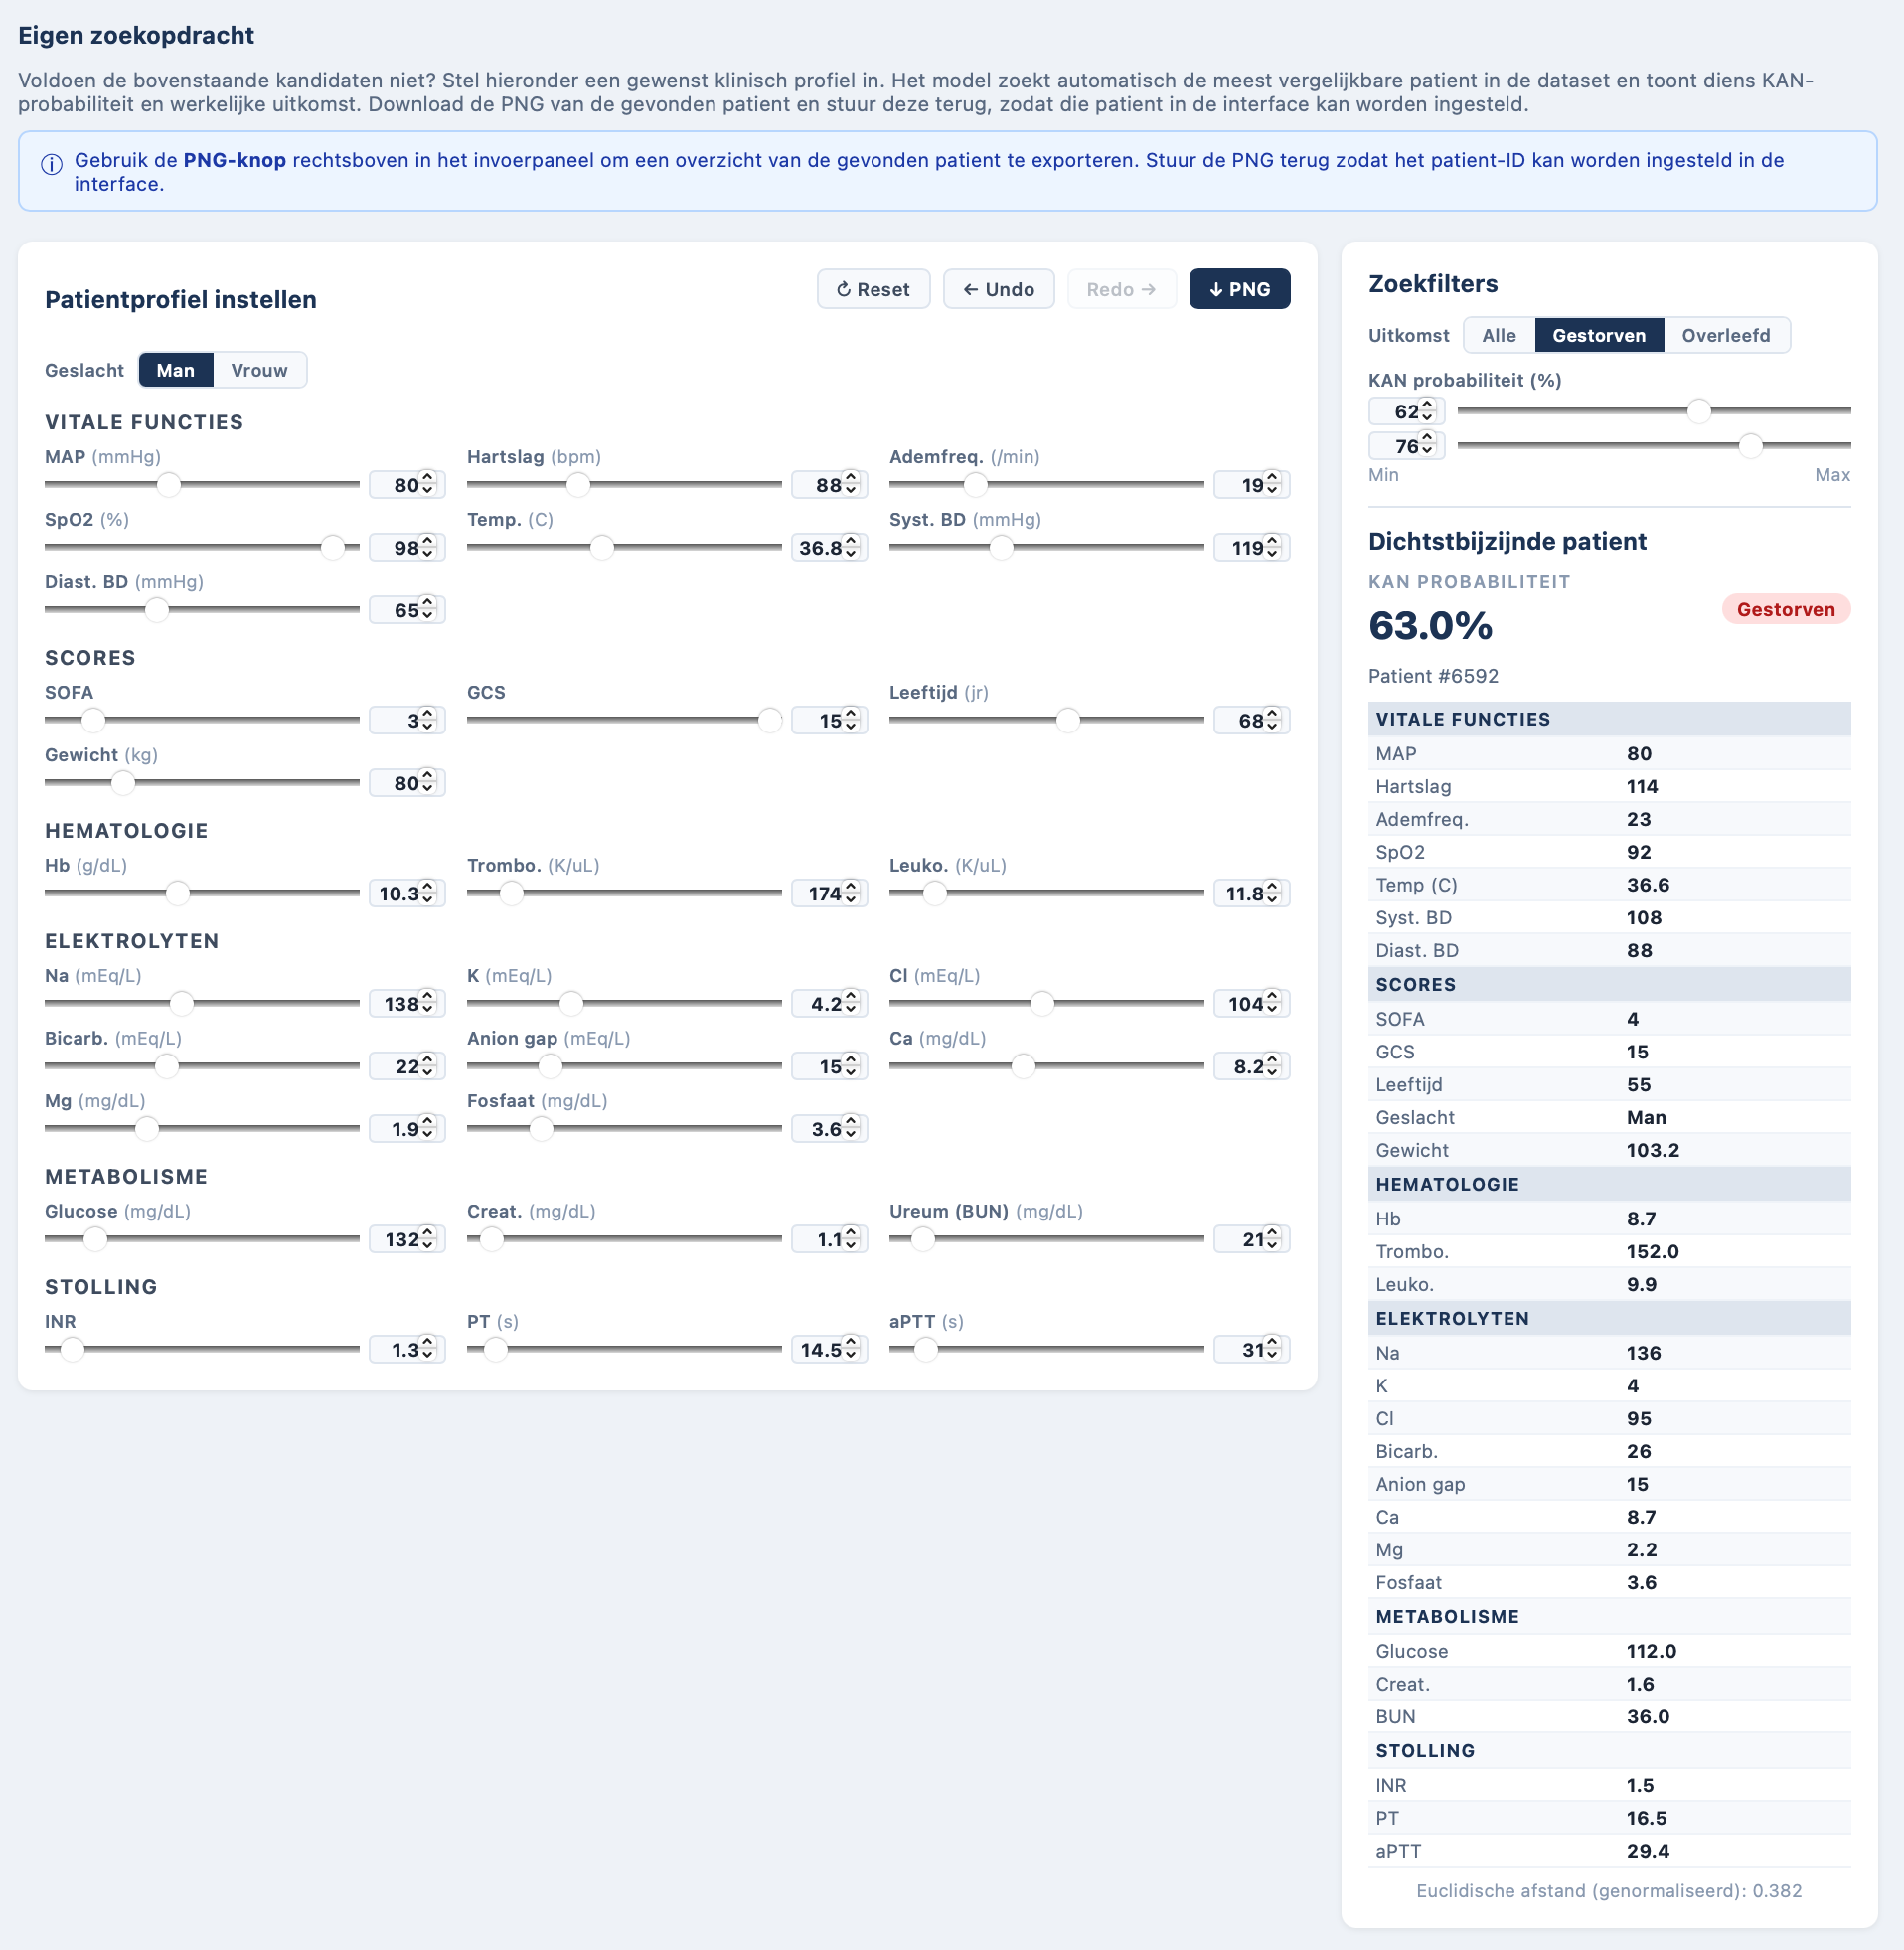
\includegraphics[width=\textwidth]{SupplementaryImages/patientCalculator.png}
  \caption{Patient calculator tool used during patient case selection. The clinician adjusts
    clinical parameters (left panel) and the tool retrieves the nearest matching patient
    from the test set (right panel) by Euclidean distance on normalised features.}
  \label{fig:patient_calc}
\end{figure}

\label{app:candidates}
Figure~\ref{fig:candidates} shows the five pre-selected candidate
patients that met the selection criteria (KAN probability 60--70\%,
actually deceased, no single immediately alarming marker). Patient
\#8259, highlighted as currently selected, was chosen by the consulting
clinician.

\begin{figure}[htbp]
  \centering
  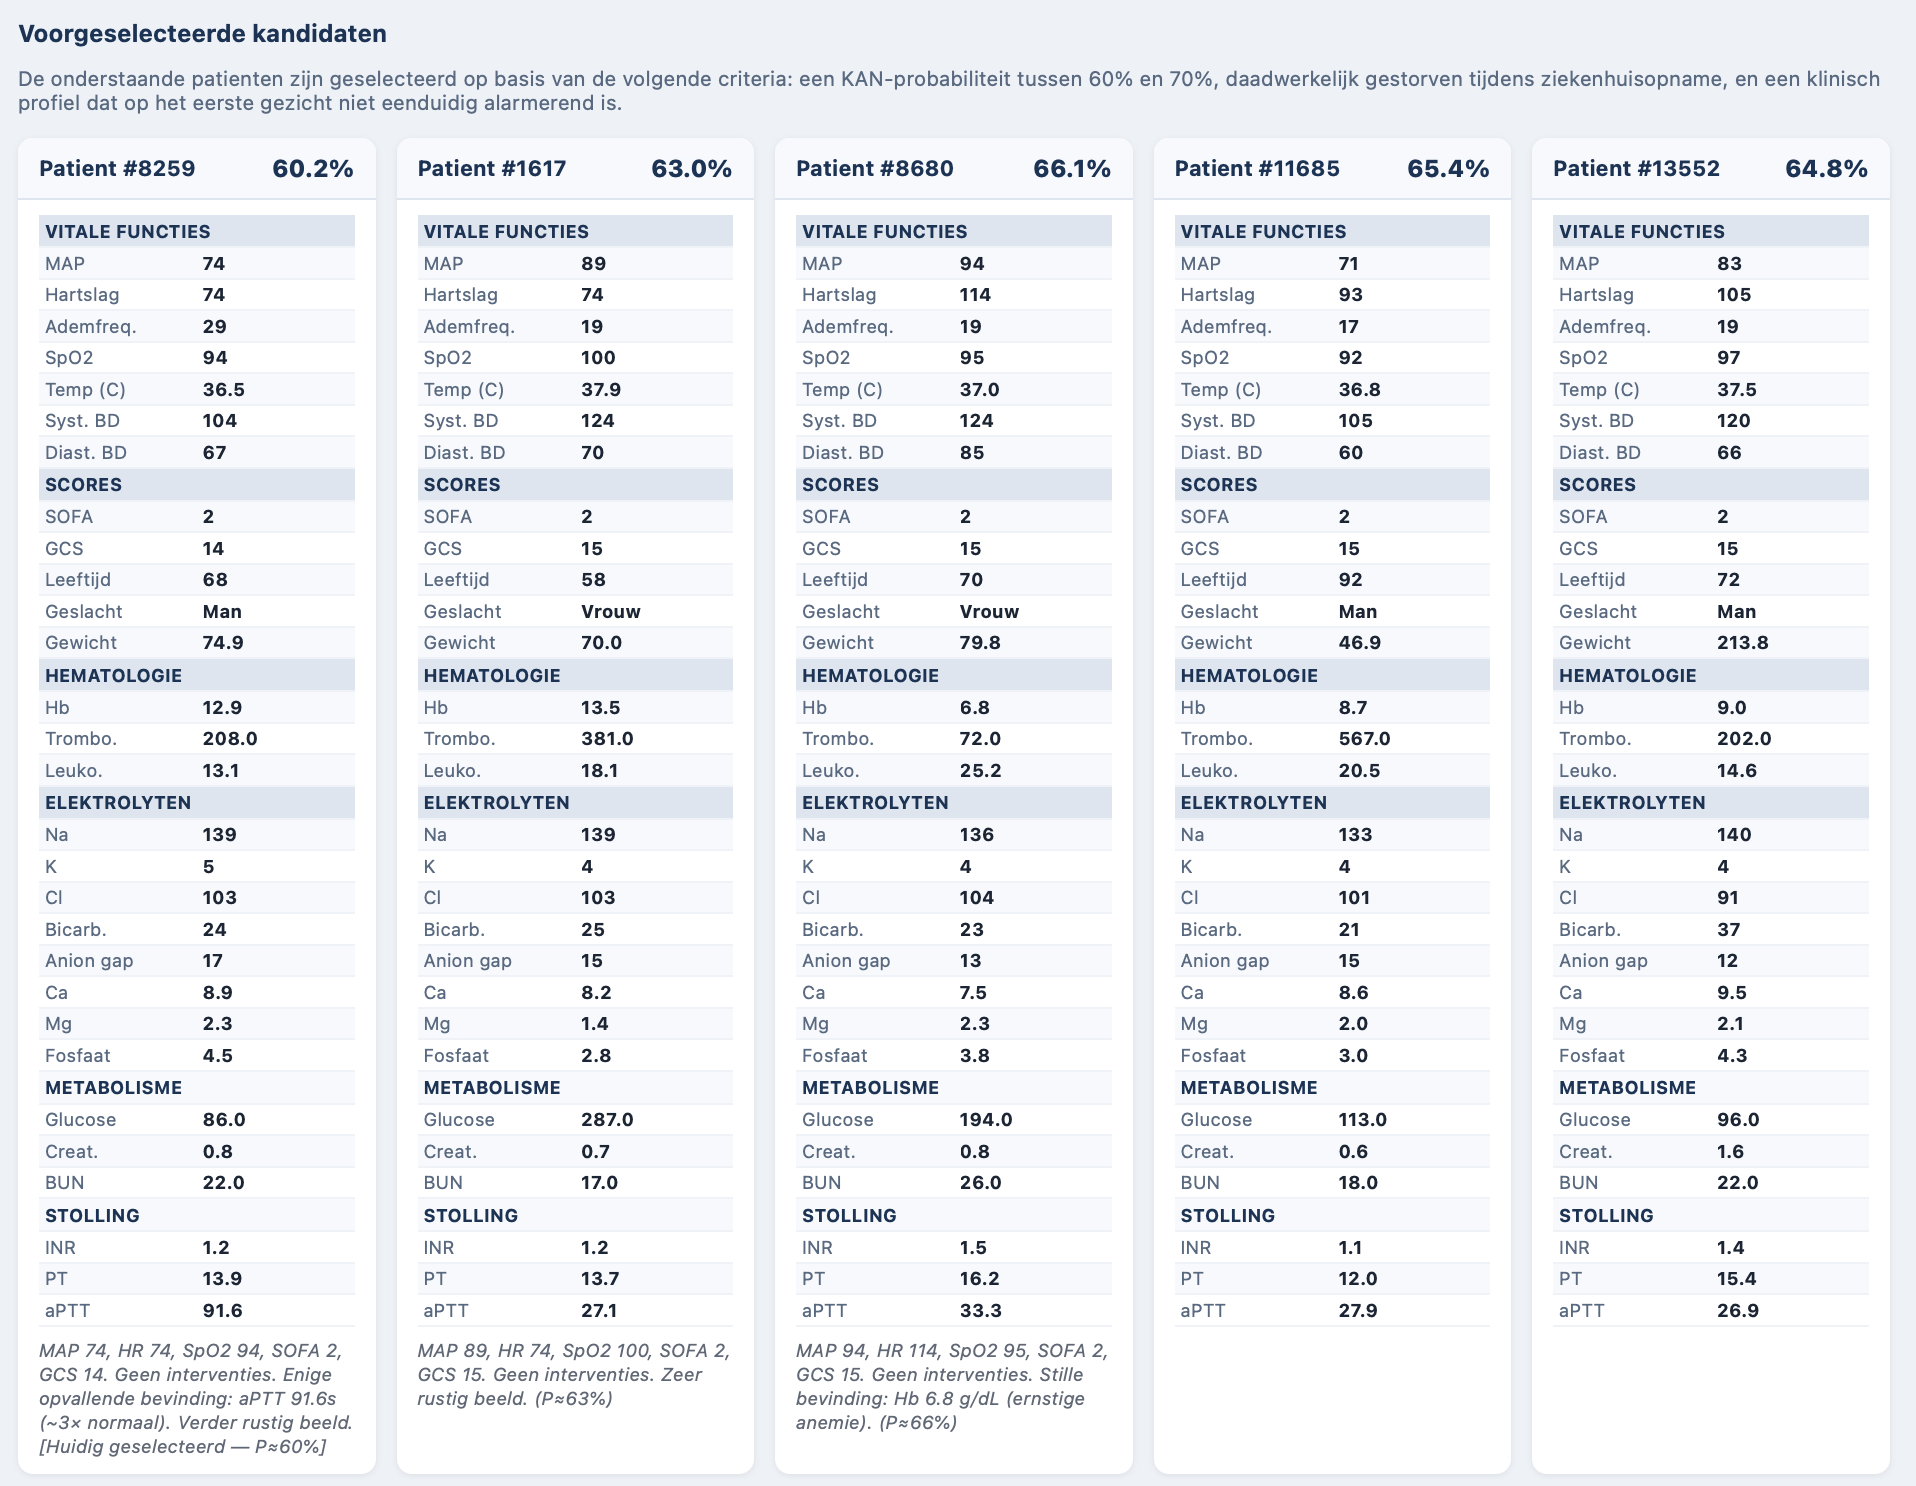
\includegraphics[width=\textwidth]{SupplementaryImages/pre-selectedCandidates.png}
  \caption{Pre-selected candidate patients meeting the edge-case criteria (KAN probability
    60--70\%, deceased, no single unambiguously alarming feature). Patient \#8259
    (currently selected, 60.2\%) was chosen as the study case.}
  \label{fig:candidates}
\end{figure}

\clearpage
\section{BigQuery Queries for Patient \#8259 Clinical Context}
\label{app:bigquery}

To construct the clinical profile shown to study participants, raw data were
retrieved from MIMIC-IV v3.1 on PhysioNet via BigQuery. Each query targets
\texttt{stay\_id}~35676599 (ICU stay) and \texttt{hadm\_id}~25820763
(hospital admission). Dates in results are in the MIMIC-IV shifted calendar
(year~2200); all timestamps are \textsc{datetime} values.
The abnormal flag column (\textbf{Abn}) uses~$*$ for flagged values.

% ─────────────────────────────────────────────────────────────────────────────
\subsection*{Query 1 --- ICU stay identifiers}

To obtain \texttt{subject\_id} and \texttt{hadm\_id} needed for all
subsequent queries, and to confirm the ICU unit and exact admission window.

\begin{lstlisting}[style=sql]
SELECT
  stay_id, subject_id, hadm_id,
  first_careunit, last_careunit,
  intime, outtime,
  DATETIME_DIFF(outtime, intime, HOUR) AS icu_hours
FROM `physionet-data.mimiciv_3_1_icu.icustays`
WHERE stay_id = 35676599
\end{lstlisting}

\medskip
\begin{table}[h]
\centering\scriptsize
\begin{tabular}{ll}
\toprule
\textbf{Field} & \textbf{Value} \\
\midrule
stay\_id        & 35676599 \\
subject\_id     & 13776612 \\
hadm\_id        & 25820763 \\
first\_careunit & MICU/SICU \\
last\_careunit  & MICU/SICU \\
intime          & 2200-07-31 19:29 \\
outtime         & 2200-08-03 23:57 \\
icu\_hours      & 76 \\
\bottomrule
\end{tabular}
\end{table}

\noindent\textbf{Finding:} Confirms linking identifiers \texttt{subject\_id}~=~13776612 and
\texttt{hadm\_id}~=~25820763 needed for all subsequent queries. The patient
remained in the MICU/SICU for the entire 76-hour ICU stay (first = last careunit).

% ─────────────────────────────────────────────────────────────────────────────
\subsection*{Query 2 --- Hospital admission and death details}

To retrieve the exact admission time, total hospital stay, where the patient
arrived from, and the time and destination of discharge (or death).

\begin{lstlisting}[style=sql]
SELECT
  hadm_id, admittime, dischtime, deathtime,
  admission_type, admission_location, discharge_location,
  DATETIME_DIFF(dischtime, admittime, HOUR) AS hosp_hours
FROM `physionet-data.mimiciv_3_1_hosp.admissions`
WHERE hadm_id = 25820763
\end{lstlisting}

\medskip
\begin{table}[h]
\centering\scriptsize
\begin{tabular}{ll}
\toprule
\textbf{Field} & \textbf{Value} \\
\midrule
hadm\_id            & 25820763 \\
admittime           & 2200-07-27 11:26 \\
dischtime           & 2200-08-03 18:40 \\
deathtime           & 2200-08-03 18:40 \\
admission\_type     & EW EMER. \\
admission\_location & EMERGENCY ROOM \\
discharge\_location & DIED \\
hosp\_hours         & 175 \\
\bottomrule
\end{tabular}
\end{table}

\noindent\textbf{Finding:} Patient admitted via the emergency room on 27~Jul;
total hospital stay 175~h ($\approx$7.3 days). Dischtime equals deathtime,
confirming in-hospital death on 3~Aug; discharge\_location = DIED.

% ─────────────────────────────────────────────────────────────────────────────
\subsection*{Query 3 --- Full hospital transfer path}

To trace the patient's complete route through the hospital and determine how
long before the model's ICU admission deterioration had been under way.

\begin{lstlisting}[style=sql]
SELECT
  transfer_id, eventtype, careunit,
  intime, outtime,
  DATETIME_DIFF(outtime, intime, HOUR) AS hours_in_unit
FROM `physionet-data.mimiciv_3_1_hosp.transfers`
WHERE hadm_id = 25820763
ORDER BY intime
\end{lstlisting}

\medskip
{\scriptsize\setlength{\tabcolsep}{4pt}
\begin{tabular}{r l p{4.2cm} l l r}
\toprule
\textbf{Transfer ID} & \textbf{Event} & \textbf{Care Unit} & \textbf{In (MM-DD HH:MM)} & \textbf{Out} & \textbf{h} \\
\midrule
37208060 & ED       & Emergency Department   & 07-26 22:02 & 07-27 11:27 & 13 \\
33975091 & admit    & Medicine/Cardiology    & 07-27 11:27 & 07-27 13:16 & 2  \\
34014453 & transfer & Hematology/Oncology    & 07-27 13:16 & 07-27 16:19 & 3  \\
39093879 & transfer & ED Observation         & 07-27 16:19 & 07-27 16:37 & 0  \\
33301092 & transfer & MICU/SICU              & 07-27 16:37 & 07-27 19:14 & 3  \\
33271491 & transfer & MICU/SICU              & 07-27 19:14 & 07-28 14:11 & 19 \\
36158942 & transfer & Hematology/Oncology    & 07-28 14:11 & 07-31 15:04 & 73 \\
32808271 & transfer & Hematology/Oncology    & 07-31 15:04 & 07-31 19:29 & 4  \\
35676599 & transfer & MICU/SICU              & 07-31 19:29 & 08-03 23:57 & 76 \\
30000088 & discharge & UNKNOWN               & 08-03 23:57 & ---         & ---\\
\bottomrule
\end{tabular}
}

\noindent\textbf{Finding:} The patient was admitted to the hospital 4~days before the
model's ICU snapshot (31~Jul). There was a prior MICU/SICU stay of 22~h
(27--28~Jul), followed by 77~h on Hematology/Oncology, before the
second MICU/SICU admission on 31~Jul that constitutes the model's stay.

% ─────────────────────────────────────────────────────────────────────────────
\subsection*{Query 4 --- All laboratory values in the first 24 hours of ICU admission}

To retrieve every individual lab draw during the first 24 hours of the ICU
stay, confirm the origin of the elevated aPTT (91.6\,s) in the model's
feature snapshot, and observe how values evolved over time.

\begin{lstlisting}[style=sql]
SELECT
  le.charttime, di.label,
  le.value, le.valuenum, le.valueuom, le.flag
FROM `physionet-data.mimiciv_3_1_hosp.labevents` le
JOIN `physionet-data.mimiciv_3_1_hosp.d_labitems` di
  ON le.itemid = di.itemid
WHERE le.hadm_id = 25820763
  AND le.charttime >= DATETIME('2200-07-31 19:29:48')
  AND le.charttime <= DATETIME('2200-08-01 19:29:48')
ORDER BY le.charttime ASC
\end{lstlisting}

\medskip
{\scriptsize\setlength{\tabcolsep}{3pt}
\begin{longtable}{l p{4.5cm} r l c}
\toprule
\textbf{Time} & \textbf{Lab} & \textbf{Value} & \textbf{Unit} & \textbf{Abn} \\
\midrule
\endfirsthead
\multicolumn{5}{l}{\small\itshape (continued)} \\
\toprule
\textbf{Time} & \textbf{Lab} & \textbf{Value} & \textbf{Unit} & \textbf{Abn} \\
\midrule
\endhead
\bottomrule
\endlastfoot
% ── ICU hour ~1 (20:24) ───────────────────────────────────────────────────
07-31 20:24 & Creatine Kinase (CK)          & 14.0   & IU/L   & $*$ \\
07-31 20:24 & NTproBNP                       & 9854.0 & pg/mL  & $*$ \\
07-31 20:24 & Troponin T                     & ---    & ng/mL  &     \\
07-31 20:24 & Creatine Kinase, MB Isoenzyme  & 1.0    & ng/mL  &     \\
% ── ICU hour ~8 (03:35) — model snapshot ─────────────────────────────────
08-01 03:35 & Sodium                         & 139.0  & mEq/L  &     \\
08-01 03:35 & Creatine Kinase, MB Isoenzyme  & 1.0    & ng/mL  &     \\
08-01 03:35 & Troponin T                     & ---    & ng/mL  &     \\
08-01 03:35 & Chloride                       & 103.0  & mEq/L  &     \\
08-01 03:35 & Glucose                        & 86.0   & mg/dL  &     \\
08-01 03:35 & PTT                            & 91.6   & sec    & $*$ \\
08-01 03:35 & Basophils                      & 0.1    & \%     &     \\
08-01 03:35 & PT                             & 13.9   & sec    & $*$ \\
08-01 03:35 & Creatinine                     & 0.8    & mg/dL  &     \\
08-01 03:35 & RDW                            & 16.3   & \%     & $*$ \\
08-01 03:35 & Platelet Count                 & 208.0  & K/uL   &     \\
08-01 03:35 & Anion Gap                      & 17.0   & mEq/L  &     \\
08-01 03:35 & INR(PT)                        & 1.2    &        & $*$ \\
08-01 03:35 & Hemoglobin                     & 12.9   & g/dL   &     \\
08-01 03:35 & White Blood Cells              & 13.1   & K/uL   & $*$ \\
08-01 03:35 & Potassium                      & 5.4    & mEq/L  & $*$ \\
08-01 03:35 & MCH                            & 29.0   & pg     &     \\
08-01 03:35 & Neutrophils                    & 88.9   & \%     & $*$ \\
08-01 03:35 & Hematocrit                     & 41.6   & \%     &     \\
08-01 03:35 & Phosphate                      & 4.5    & mg/dL  &     \\
08-01 03:35 & Calcium, Total                 & 8.9    & mg/dL  &     \\
08-01 03:35 & Lymphocytes                    & 5.5    & \%     & $*$ \\
08-01 03:35 & Magnesium                      & 2.3    & mg/dL  &     \\
08-01 03:35 & Monocytes                      & 5.0    & \%     &     \\
08-01 03:35 & MCHC                           & 30.9   & \%     & $*$ \\
08-01 03:35 & Urea Nitrogen                  & 22.0   & mg/dL  & $*$ \\
08-01 03:35 & Eosinophils                    & 0.5    & \%     &     \\
08-01 03:35 & Red Blood Cells                & 4.44   & m/uL   &     \\
08-01 03:35 & Bicarbonate                    & 24.0   & mEq/L  &     \\
08-01 03:35 & MCV                            & 94.0   & fL     &     \\
08-01 03:35 & Creatine Kinase (CK)           & 35.0   & IU/L   &     \\
% ── ICU hour ~10 (05:57) — urinalysis ────────────────────────────────────
08-01 05:57 & Blood                          & ---    &        &     \\
08-01 05:57 & Bilirubin                      & ---    & mg/dL  &     \\
08-01 05:57 & Leukocytes                     & ---    &        &     \\
08-01 05:57 & Ketone                         & ---    & mg/dL  &     \\
08-01 05:57 & Urine Color                    & ---    &        &     \\
08-01 05:57 & pH                             & 5.5    & units  &     \\
08-01 05:57 & Urobilinogen                   & 4.0    & mg/dL  & $*$ \\
08-01 05:57 & Specific Gravity               & 1.021  &        &     \\
08-01 05:57 & Nitrite                        & ---    &        &     \\
08-01 05:57 & Glucose                        & ---    & mg/dL  &     \\
08-01 05:57 & Urine Appearance               & ---    &        &     \\
08-01 05:57 & Protein                        & 30.0   & mg/dL  &     \\
% ── ICU hour ~13 (08:30) — venous blood gas ──────────────────────────────
08-01 08:30 & Calculated Total CO2           & 30.0   & mEq/L  &     \\
08-01 08:30 & Intubated                      & \multicolumn{2}{l}{NOT INTUBATED} &  \\
08-01 08:30 & Ventilation Rate               & \multicolumn{2}{l}{/24} &          \\
08-01 08:30 & pH                             & 7.24   & units  & $*$ \\
08-01 08:30 & Specimen Type                  & \multicolumn{2}{l}{VEN.} &         \\
08-01 08:30 & pO2                            & 51.0   & mmHg   & $*$ \\
08-01 08:30 & Base Excess                    & 0.0    & mEq/L  &     \\
08-01 08:30 & pCO2                           & 67.0   & mmHg   & $*$ \\
% ── ICU hour ~20 (15:53) — urine chemistry ───────────────────────────────
08-01 15:53 & Urea Nitrogen, Urine           & 327.0  & mg/dL  &     \\
08-01 15:53 & Length of Urine Collection     & ---    &        &     \\
08-01 15:53 & Chloride, Urine                & 43.0   & mEq/L  &     \\
08-01 15:53 & Osmolality, Urine              & 424.0  & mOsm/kg&     \\
08-01 15:53 & Potassium, Urine               & 31.0   & mEq/L  &     \\
08-01 15:53 & Urine tube, held               & ---    &        &     \\
08-01 15:53 & Sodium, Urine                  & 46.0   & mEq/L  &     \\
08-01 15:53 & Creatinine, Urine              & 82.0   & mg/dL  &     \\
% ── ICU hour ~21 (16:42) — repeat panel ──────────────────────────────────
08-01 16:42 & Sodium                         & 136.0  & mEq/L  &     \\
08-01 16:42 & Calcium, Total                 & 7.8    & mg/dL  & $*$ \\
08-01 16:42 & Magnesium                      & 1.9    & mg/dL  &     \\
08-01 16:42 & Bicarbonate                    & 25.0   & mEq/L  &     \\
08-01 16:42 & Potassium                      & 4.4    & mEq/L  &     \\
08-01 16:42 & RDW                            & 17.0   & \%     & $*$ \\
08-01 16:42 & MCHC                           & 29.6   & \%     & $*$ \\
08-01 16:42 & MCV                            & 96.0   & fL     &     \\
08-01 16:42 & White Blood Cells              & 12.4   & K/uL   & $*$ \\
08-01 16:42 & Urea Nitrogen                  & 22.0   & mg/dL  & $*$ \\
08-01 16:42 & Red Blood Cells                & 4.30   & m/uL   &     \\
08-01 16:42 & Hemoglobin                     & 12.2   & g/dL   &     \\
08-01 16:42 & Creatinine                     & 0.8    & mg/dL  &     \\
08-01 16:42 & Chloride                       & 99.0   & mEq/L  &     \\
08-01 16:42 & Phosphate                      & 6.3    & mg/dL  & $*$ \\
08-01 16:42 & Hematocrit                     & 41.3   & \%     &     \\
08-01 16:42 & Platelet Count                 & 227.0  & K/uL   &     \\
08-01 16:42 & Glucose                        & 246.0  & mg/dL  & $*$ \\
08-01 16:42 & Anion Gap                      & 16.0   & mEq/L  &     \\
08-01 16:42 & MCH                            & 28.4   & pg     &     \\
% ── ICU hour ~21 (16:44) — repeat coag (empty) ───────────────────────────
08-01 16:44 & PT                             & ---    & sec    &     \\
08-01 16:44 & INR(PT)                        & ---    &        &     \\
08-01 16:44 & PTT                            & ---    & sec    &     \\
% ── ICU hour ~23 (18:46) — repeat coag ───────────────────────────────────
08-01 18:46 & INR(PT)                        & 1.2    &        & $*$ \\
08-01 18:46 & PTT                            & 150.0  & sec    & $*$ \\
08-01 18:46 & PT                             & 13.1   & sec    & $*$ \\
\end{longtable}
}

\noindent\textbf{Finding:} The model's 29-feature snapshot corresponds to the 03:35 lab
draw (ICU hour~8). PTT~=~91.6\,s, INR~=~1.2, potassium~=~5.4\,mEq/L, and all
other model input values are confirmed at that timepoint.

% ─────────────────────────────────────────────────────────────────────────────
\subsection*{Query 5 --- ICD-10 discharge diagnoses}

To retrieve the coded discharge diagnoses and establish the primary clinical
reason for admission, clarify the source of the elevated aPTT, and understand
why an acute kidney injury flag was present despite near-normal creatinine.

\begin{lstlisting}[style=sql]
SELECT
  seq_num, icd_code, icd_version,
  d.long_title
FROM `physionet-data.mimiciv_3_1_hosp.diagnoses_icd` diag
JOIN `physionet-data.mimiciv_3_1_hosp.d_icd_diagnoses` d
  USING (icd_code, icd_version)
WHERE hadm_id = 25820763
ORDER BY seq_num
\end{lstlisting}

\medskip
{\scriptsize\setlength{\tabcolsep}{4pt}
\begin{longtable}{r l r p{8cm}}
\toprule
\textbf{\#} & \textbf{ICD Code} & \textbf{Ver.} & \textbf{Diagnosis} \\
\midrule
\endfirsthead
\multicolumn{4}{l}{\small\itshape (continued)} \\
\toprule
\textbf{\#} & \textbf{ICD Code} & \textbf{Ver.} & \textbf{Diagnosis} \\
\midrule
\endhead
\bottomrule
\endlastfoot
 1 & 162.9   & 9 & Malignant neoplasm of bronchus and lung, unspecified \\
 2 & 486     & 9 & Pneumonia, organism unspecified \\
 3 & 707.23  & 9 & Pressure ulcer, stage III \\
 4 & 342.80  & 9 & Other specified hemiplegia and hemiparesis, unspecified side \\
 5 & 682.5   & 9 & Cellulitis and abscess of buttock \\
 6 & 428.32  & 9 & Chronic diastolic heart failure \\
 7 & 427.31  & 9 & Atrial fibrillation \\
 8 & V45.76  & 9 & Acquired absence of organ, lung \\
 9 & 416.8   & 9 & Other chronic pulmonary heart diseases \\
10 & 714.0   & 9 & Rheumatoid arthritis \\
11 & 300.00  & 9 & Anxiety state, unspecified \\
12 & 401.9   & 9 & Unspecified essential hypertension \\
13 & V15.82  & 9 & Personal history of tobacco use \\
14 & 707.05  & 9 & Pressure ulcer, buttock \\
15 & 707.07  & 9 & Pressure ulcer, heel \\
16 & 707.20  & 9 & Pressure ulcer, unspecified stage \\
17 & 428.0   & 9 & Congestive heart failure, unspecified \\
18 & 345.90  & 9 & Epilepsy, unspecified, without intractable epilepsy \\
19 & V49.86  & 9 & Do not resuscitate status \\
20 & V66.7   & 9 & Encounter for palliative care \\
21 & 788.5   & 9 & Oliguria and anuria \\
22 & 041.12  & 9 & Methicillin-resistant \textit{Staphylococcus aureus} (MRSA) \\
\end{longtable}
}

\noindent\textbf{Finding:} Atrial fibrillation (seq~7) provides the clinical context for
heparin therapy, explaining why PTT~=~91.6\,s (a direct model input) is
elevated while INR remains at~1.2.

% ─────────────────────────────────────────────────────────────────────────────
\subsection*{Query 6 --- Medications administered before the lab draw}

To retrieve all fluids and medications administered in the ICU prior to the
lab snapshot at 03:35 (ICU hour~8), providing context for the elevated aPTT
and the treatment trajectory up to that point.

\begin{lstlisting}[style=sql]
SELECT
  di.label AS medication,
  ie.starttime, ie.endtime,
  ie.amount, ie.amountuom,
  ie.rate, ie.rateuom
FROM `physionet-data.mimiciv_3_1_icu.inputevents` ie
JOIN `physionet-data.mimiciv_3_1_icu.d_items` di
  ON ie.itemid = di.itemid
WHERE ie.stay_id = 35676599
  AND ie.starttime < DATETIME('2200-08-01 03:35:00')
ORDER BY ie.starttime
\end{lstlisting}

\medskip
{\scriptsize\setlength{\tabcolsep}{3pt}
\begin{tabular}{p{2.8cm} l l r l r l}
\toprule
\textbf{Medication} & \textbf{Start} & \textbf{End} & \textbf{Amount} & \textbf{Unit} & \textbf{Rate} & \textbf{Rate unit} \\
\midrule
Dextrose 5\%      & 07-31 19:45 & 08-01 11:50 & 249.5   & mL    & 15.5    & mL/hour \\
Heparin Sodium    & 07-31 19:45 & 08-01 11:50 & 24950.0 & units & 1551.3  & units/hour \\
Bactrim (SMX/TMP) & 07-31 20:00 & 07-31 20:01 & 1.0     & dose  & ---     & --- \\
NaCl 0.9\%        & 08-01 02:34 & 08-01 03:34 & 500.0   & mL    & 500.0   & mL/hour \\
\bottomrule
\end{tabular}
}

\noindent\textbf{Finding:} Heparin sodium was commenced immediately at ICU admission
(19:45) at 1551 units/h (running continuously up to the lab draw and beyond),
confirming anticoagulation therapy as the cause of PTT~=~91.6\,s. Bactrim
(trimethoprim-sulfamethoxazole) was administered as a single dose at 20:00.
NaCl 0.9\% was given as a 500\,mL/h bolus in the hour immediately preceding
the 03:35 lab draw.

\clearpage
\section{Study Interface Screenshots}
\label{app:interface}

All screens are reproduced as shown to participants (Dutch language),
with full English translations provided below each figure.

% ── Screen 0: Welcome ─────────────────────────────────────────────────────────
\begin{figure}[htbp]
  \centering
  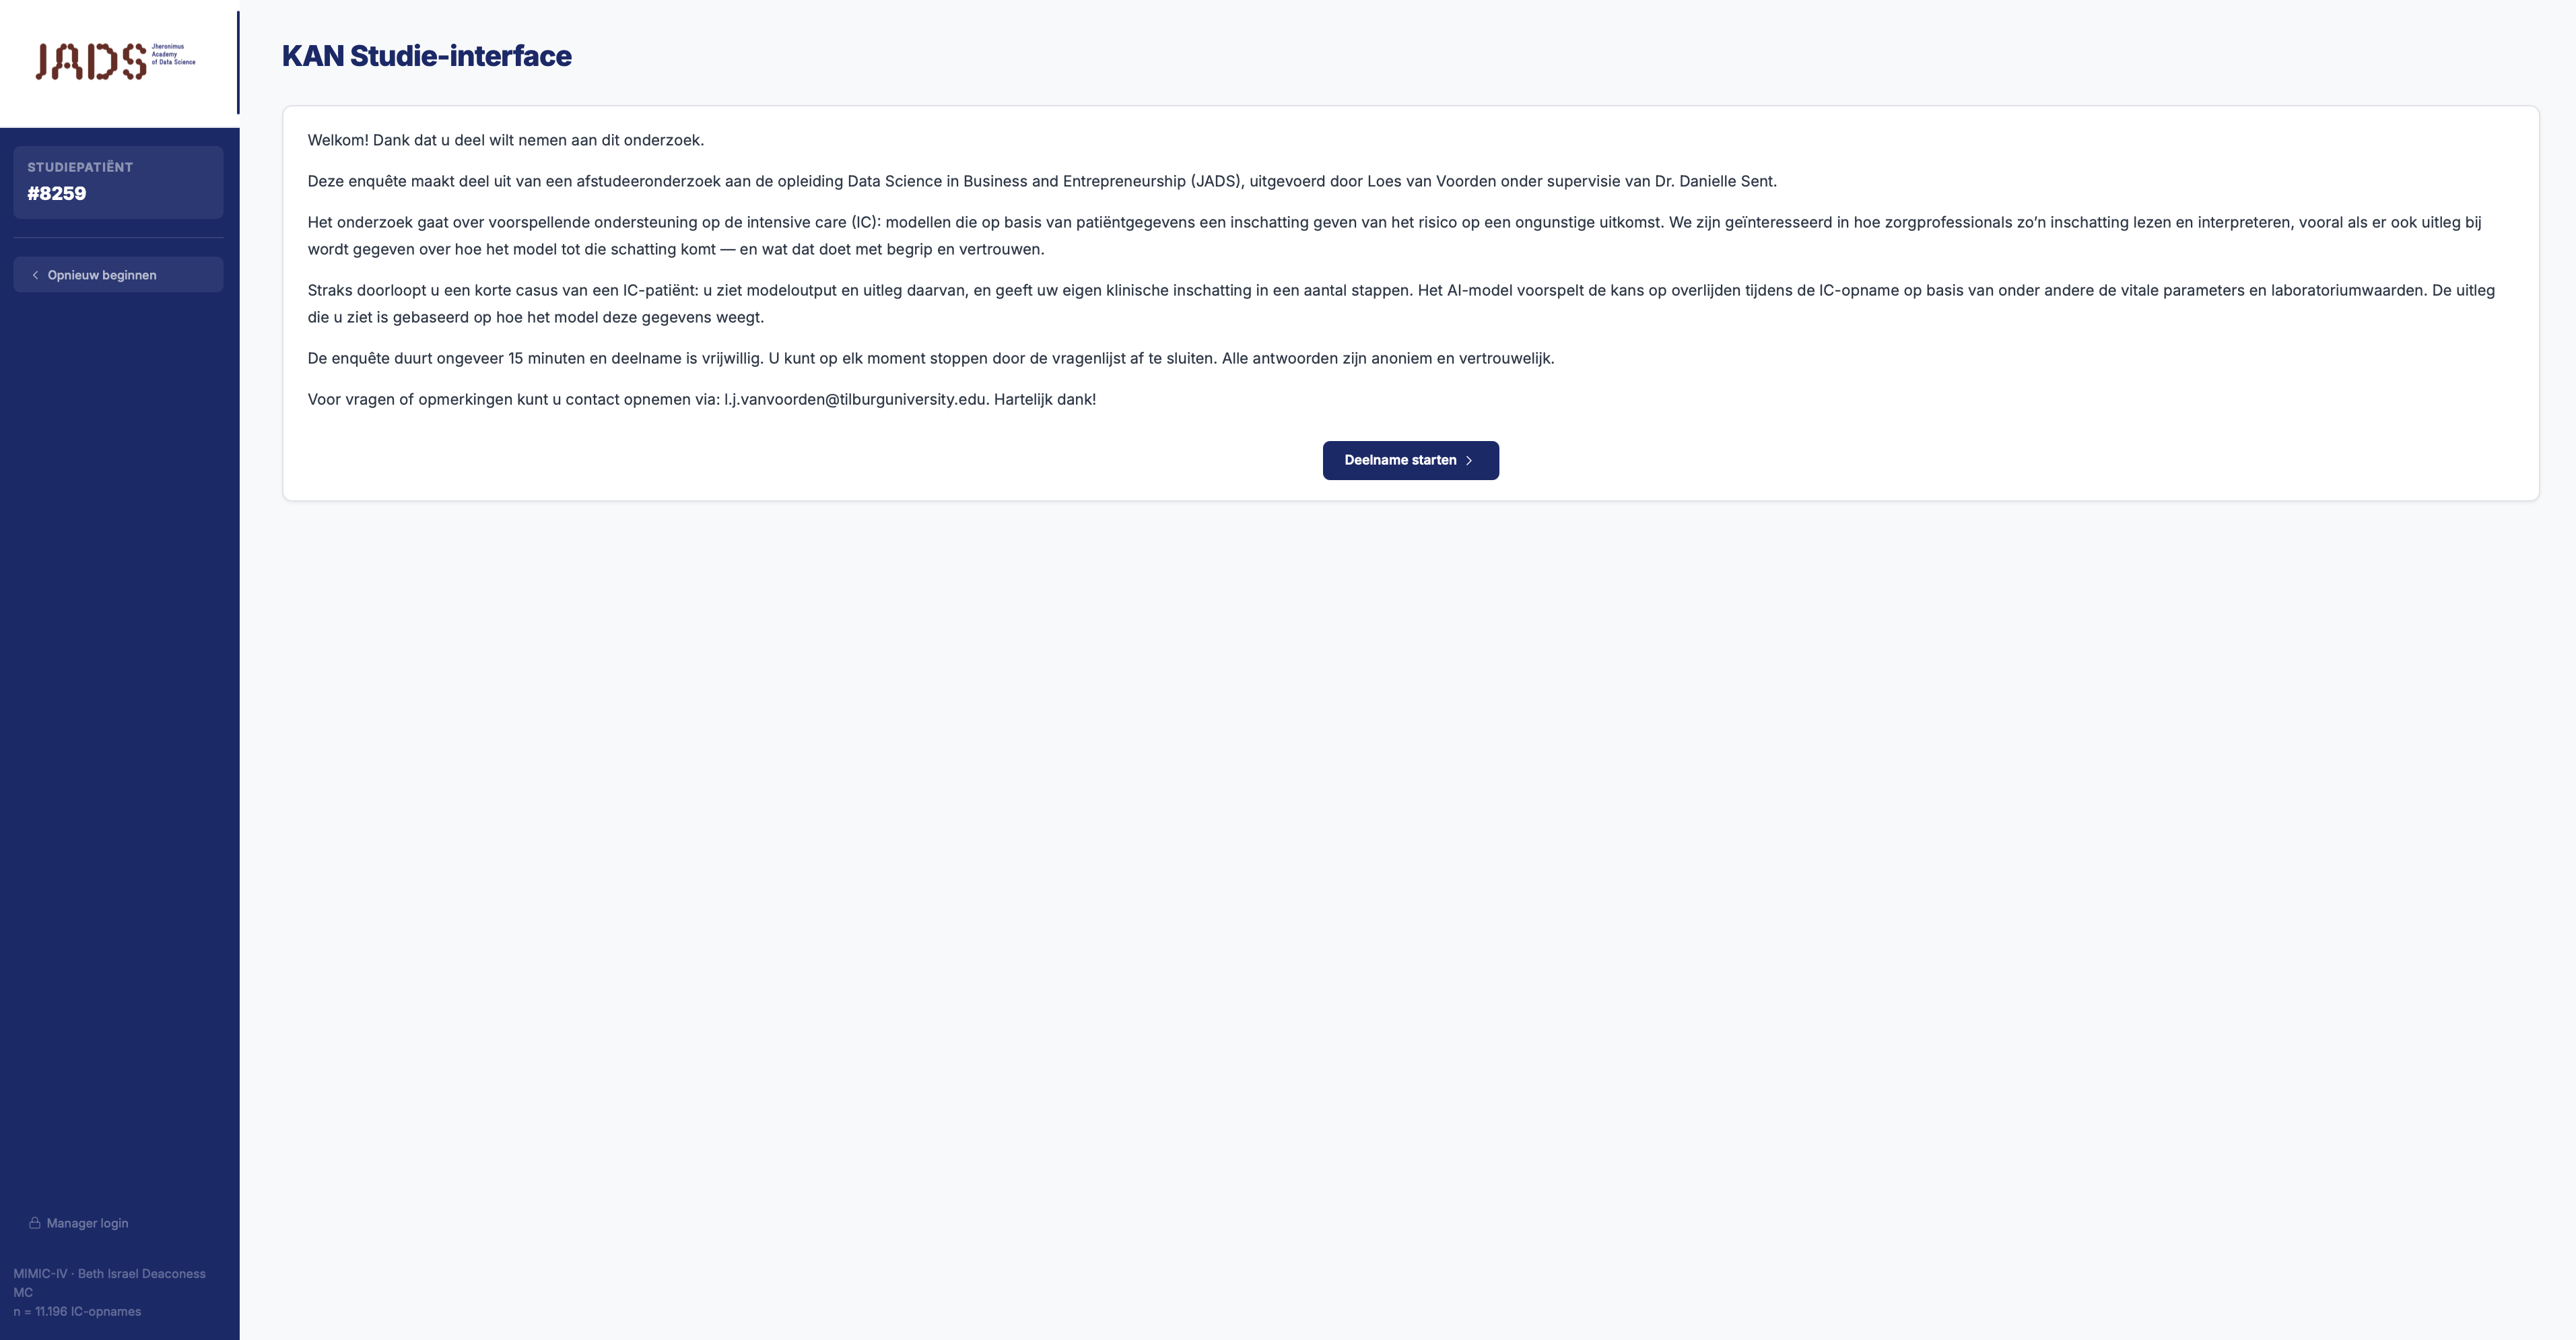
\includegraphics[width=\textwidth]{SupplementaryImages/screenOpening.png}
  \caption[Welcome screen]{Welcome and information screen shown to all
    participants before the study begins.}
  \label{fig:screen_opening}
\end{figure}

\noindent\textit{Translation (screenOpening):}

\smallskip\noindent\textbf{KAN Study Interface}

\smallskip\noindent Welcome! Thank you for your willingness to participate
in this study.

\smallskip\noindent This survey is part of a master's thesis in the Data
Science in Business and Entrepreneurship programme (JADS), conducted by
Loes van Voorden under the supervision of Dr.\ Dani\"{e}lle Sent.

\smallskip\noindent The research concerns predictive decision support in
the intensive care unit (ICU): models that estimate the risk of an adverse
outcome based on patient data. We are interested in how healthcare
professionals read and interpret such estimates, especially when an
explanation of how the model arrived at the prediction is provided ---
and what effect this has on understanding and trust.

\smallskip\noindent Shortly you will work through a brief ICU patient case:
you will see model output, an explanation of it, and provide your own
clinical assessment in several steps. The AI model predicts the probability
of death during the hospital admission based on, among other things, vital
parameters and laboratory values. The explanation you see is based on how
the model weighs this data.

\smallskip\noindent The survey takes approximately 15 minutes and
participation is voluntary. You may stop at any time by closing the
questionnaire. All answers are anonymous and confidential.

\smallskip\noindent For questions or comments, contact:
\texttt{l.j.vanvoorden@tilburguniversity.edu}. Many thanks!

% ── Screen 1: Profile ─────────────────────────────────────────────────────────
\clearpage
\begin{figure}[htbp]
  \centering
  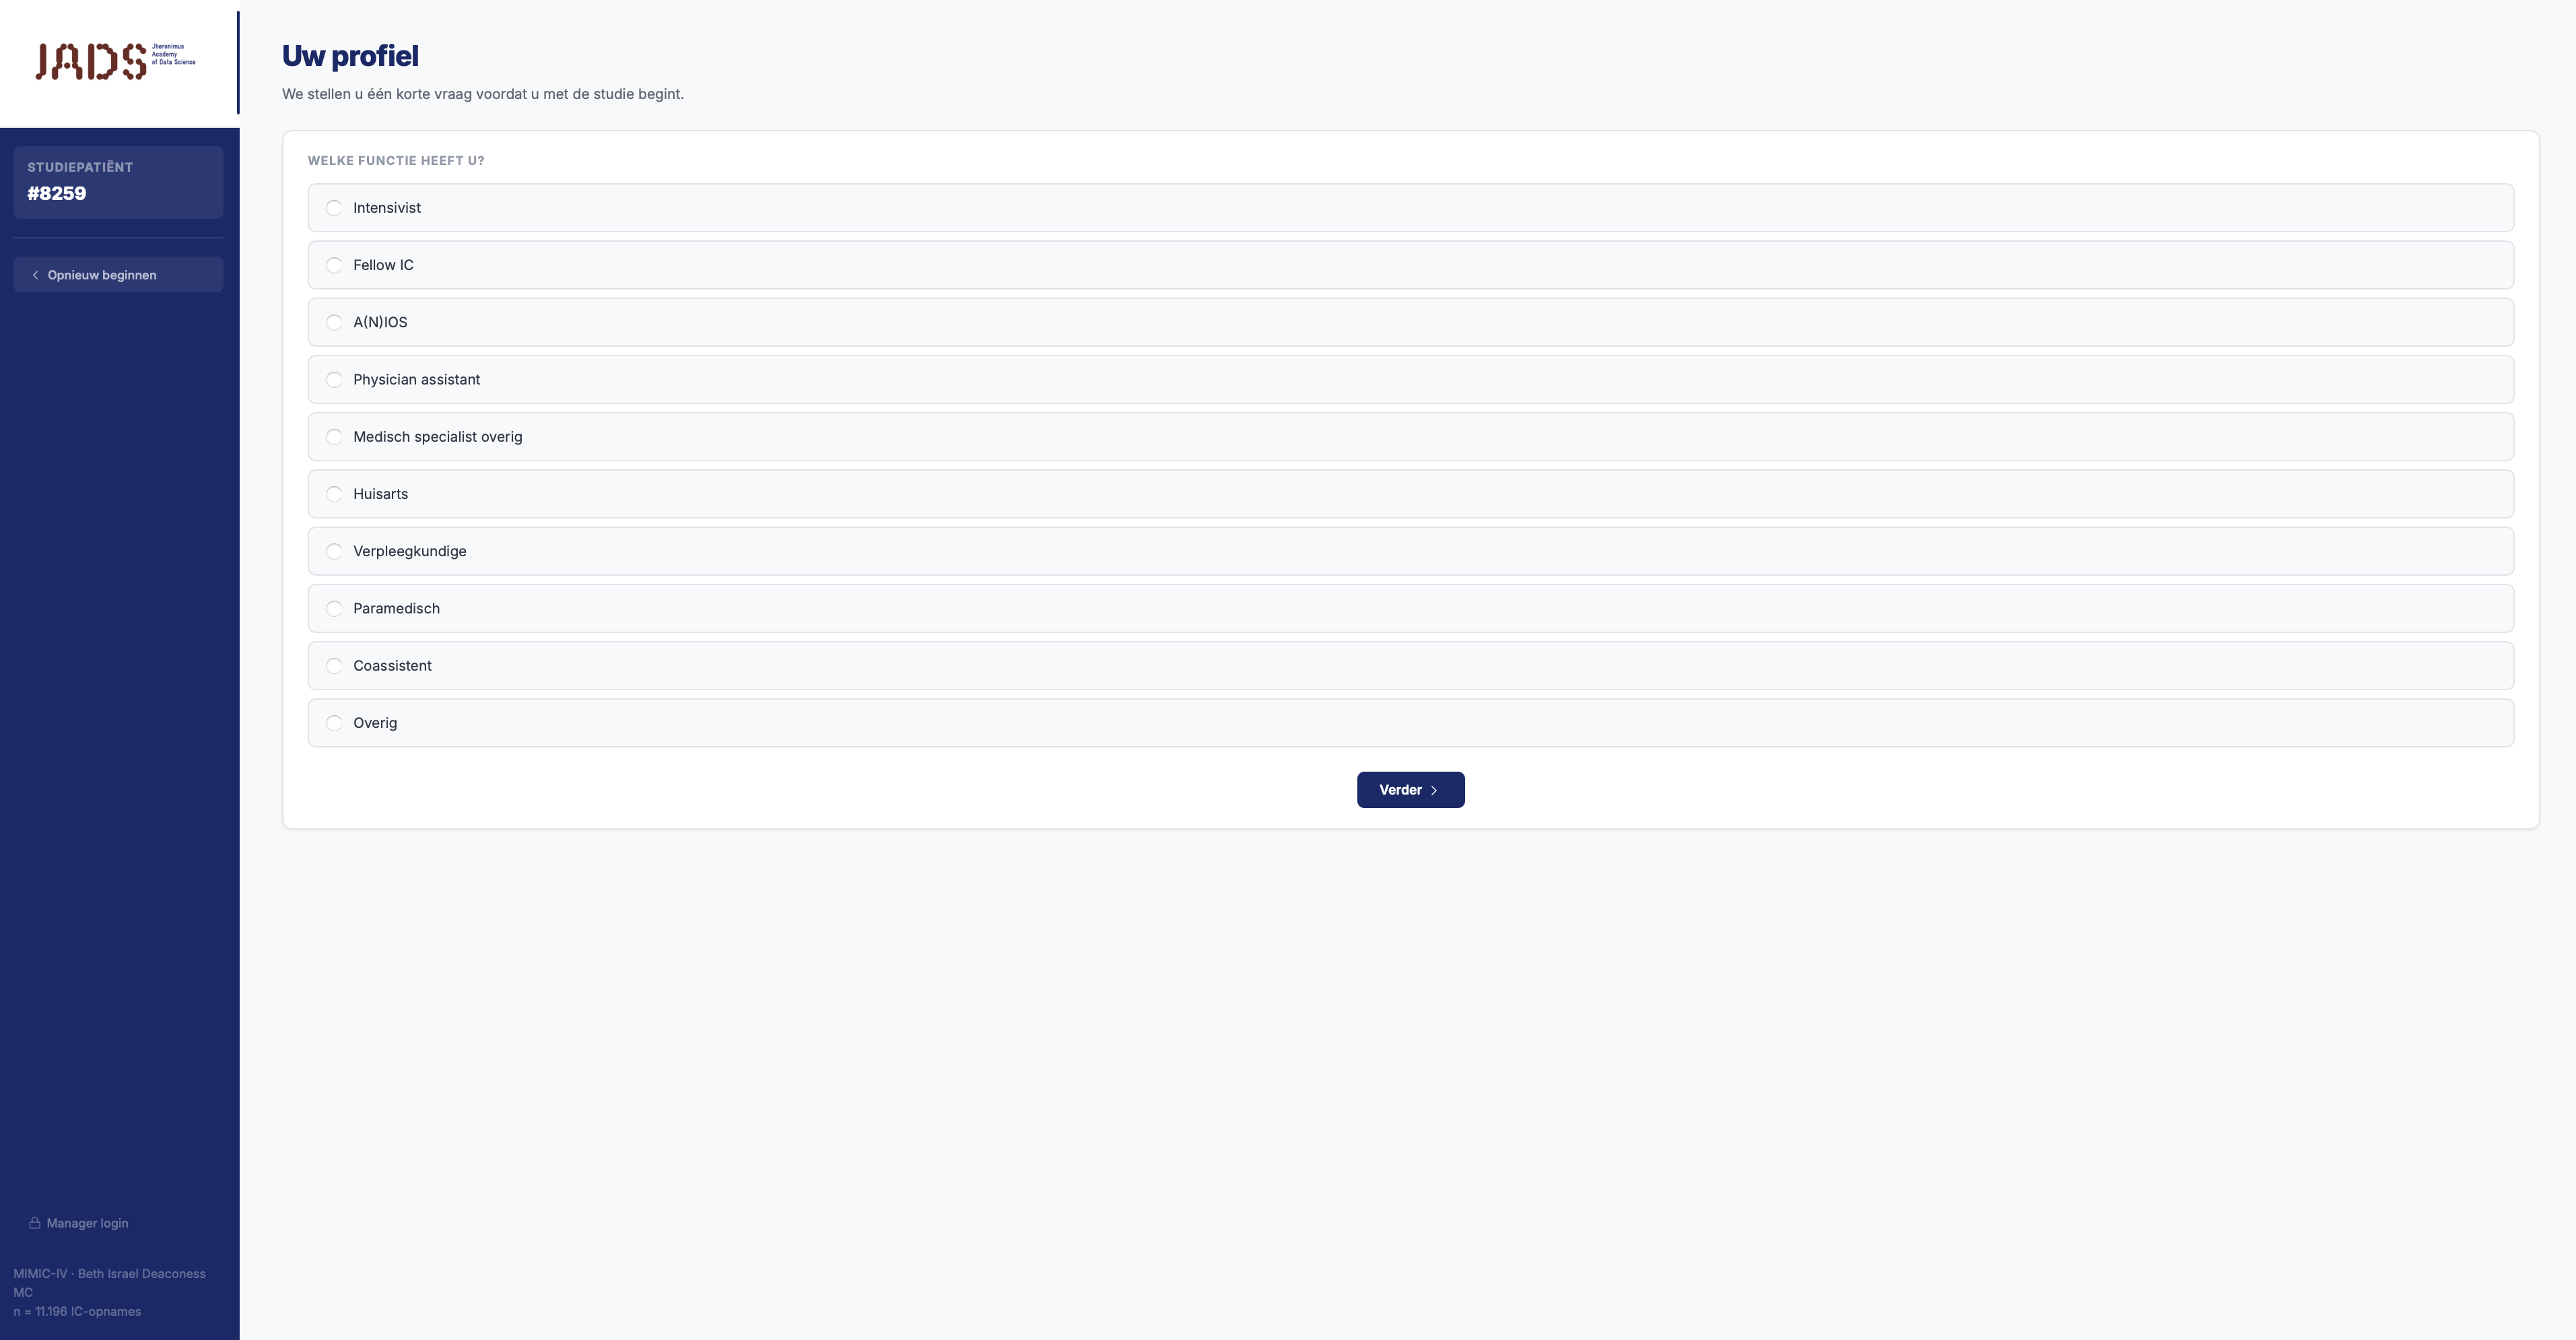
\includegraphics[width=\textwidth]{SupplementaryImages/screenProfile.png}
  \caption[Professional role screen]{Professional role screen shown before
    the patient case.}
  \label{fig:screen_profile}
\end{figure}

\noindent\textit{Translation (screenProfile):}

\smallskip\noindent\textbf{Your profile}

\smallskip\noindent We ask you one brief question before you begin the study.

\smallskip\noindent\textsc{What is your professional role?}

\smallskip Intensivist \textbar{} ICU Fellow \textbar{} Junior Doctor
(ANIOS) \textbar{} Physician Assistant \textbar{} Other Medical Specialist
\textbar{} General Practitioner \textbar{} Nurse \textbar{} Paramedic
\textbar{} Medical Student (Co-assistant) \textbar{} Other

% ── Screen 2: Blind assessment ────────────────────────────────────────────────
\clearpage
\begin{figure}[htbp]
  \centering
  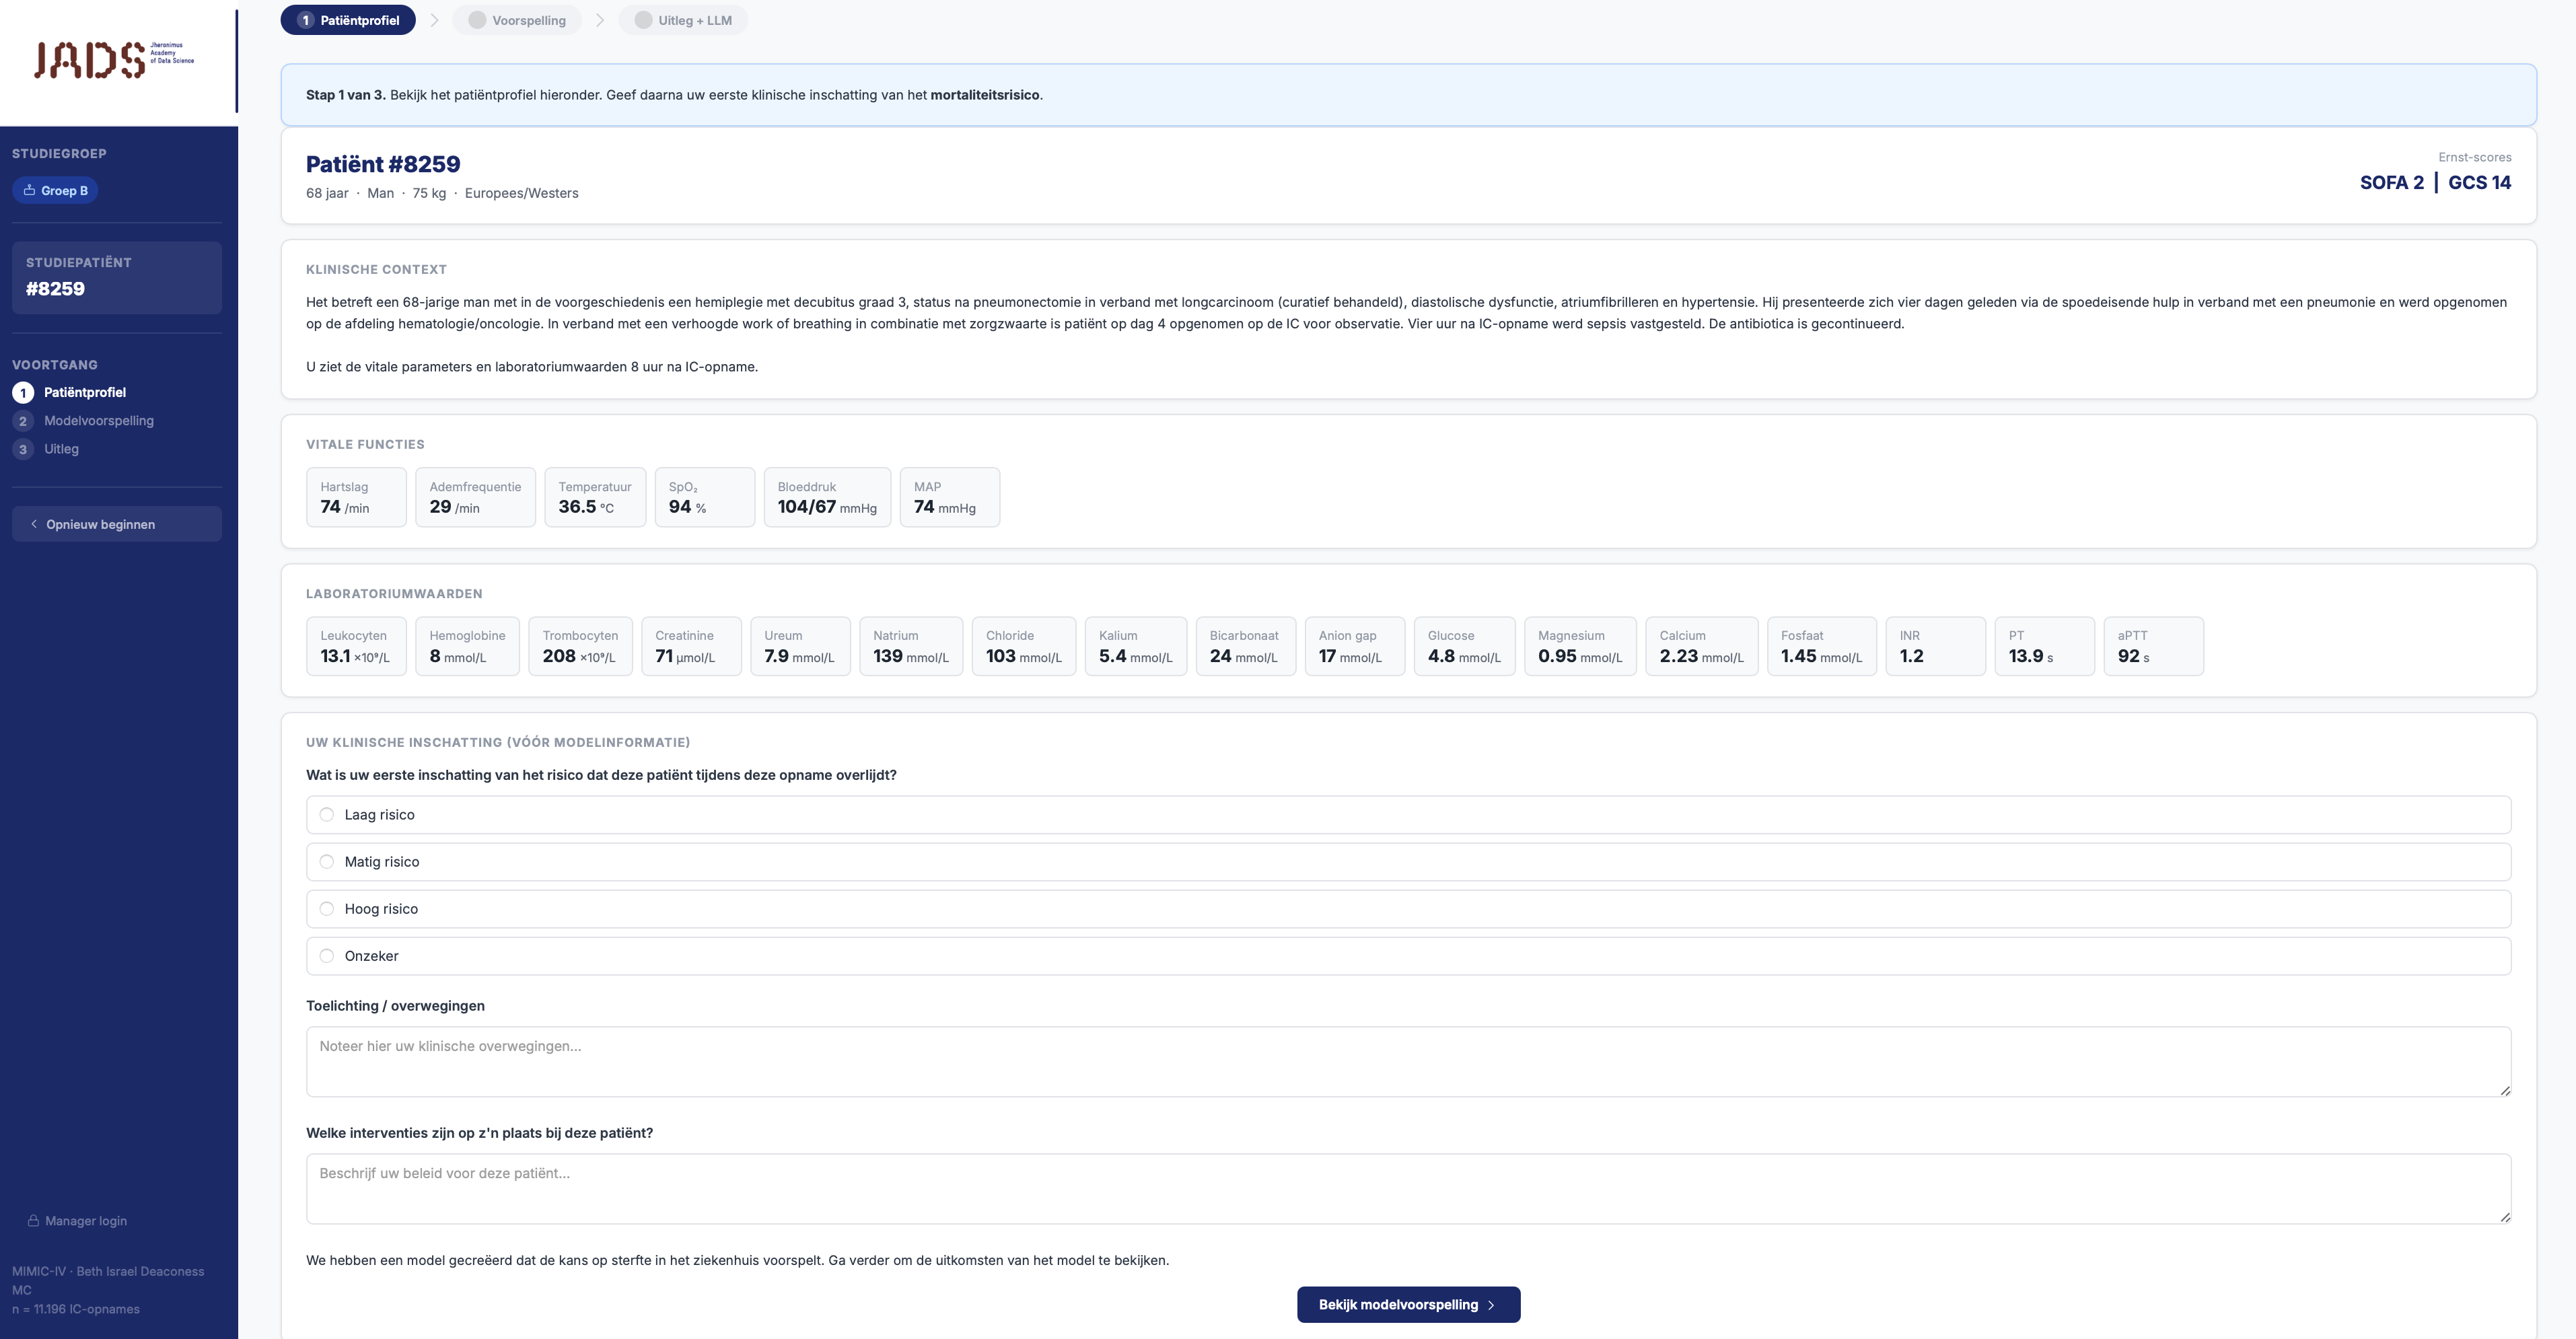
\includegraphics[width=\textwidth]{SupplementaryImages/screen1.png}
  \caption[Step~1: Blind assessment]{Step~1: Patient profile without model
    output. The screen shows the patient header, clinical context narrative,
    vital signs, and laboratory values.}
  \label{fig:screen1}
\end{figure}

\noindent\textit{Translation (screen1):}

\smallskip\noindent\textbf{Clinical Context}

\smallskip\noindent This concerns a 68-year-old man with a history of
hemiplegia and grade~III pressure ulcer, status post pneumonectomy for lung
carcinoma (treated with curative intent), diastolic dysfunction, atrial
fibrillation and hypertension. He presented four days ago via the emergency
department with pneumonia and was admitted to the haematology/oncology ward.
Due to increased work of breathing combined with nursing-care complexity,
the patient was admitted to the ICU on day~4 for observation. Sepsis was
established four hours after ICU admission. Antibiotic therapy was continued.

\smallskip\noindent You are viewing the vital signs and laboratory values
eight hours after ICU admission.

\smallskip\noindent\textsc{Your clinical assessment (before model output)}

\smallskip\noindent\textbf{(Q1)} What is your initial assessment of the
risk that this patient will die during this admission?
\emph{(Low risk / Moderate risk / High risk / Uncertain)}

\smallskip\noindent\textbf{(Q2)} Explanation / considerations (free text)

\smallskip\noindent\textbf{(Q3)} What interventions are appropriate for
this patient? (free text)

\smallskip\noindent\textit{Bottom note:} ``We have developed a model that
predicts the probability of in-hospital death. Continue to view the model
output.''

% ── Screen 3: Model prediction ────────────────────────────────────────────────
\clearpage
\begin{figure}[htbp]
  \centering
  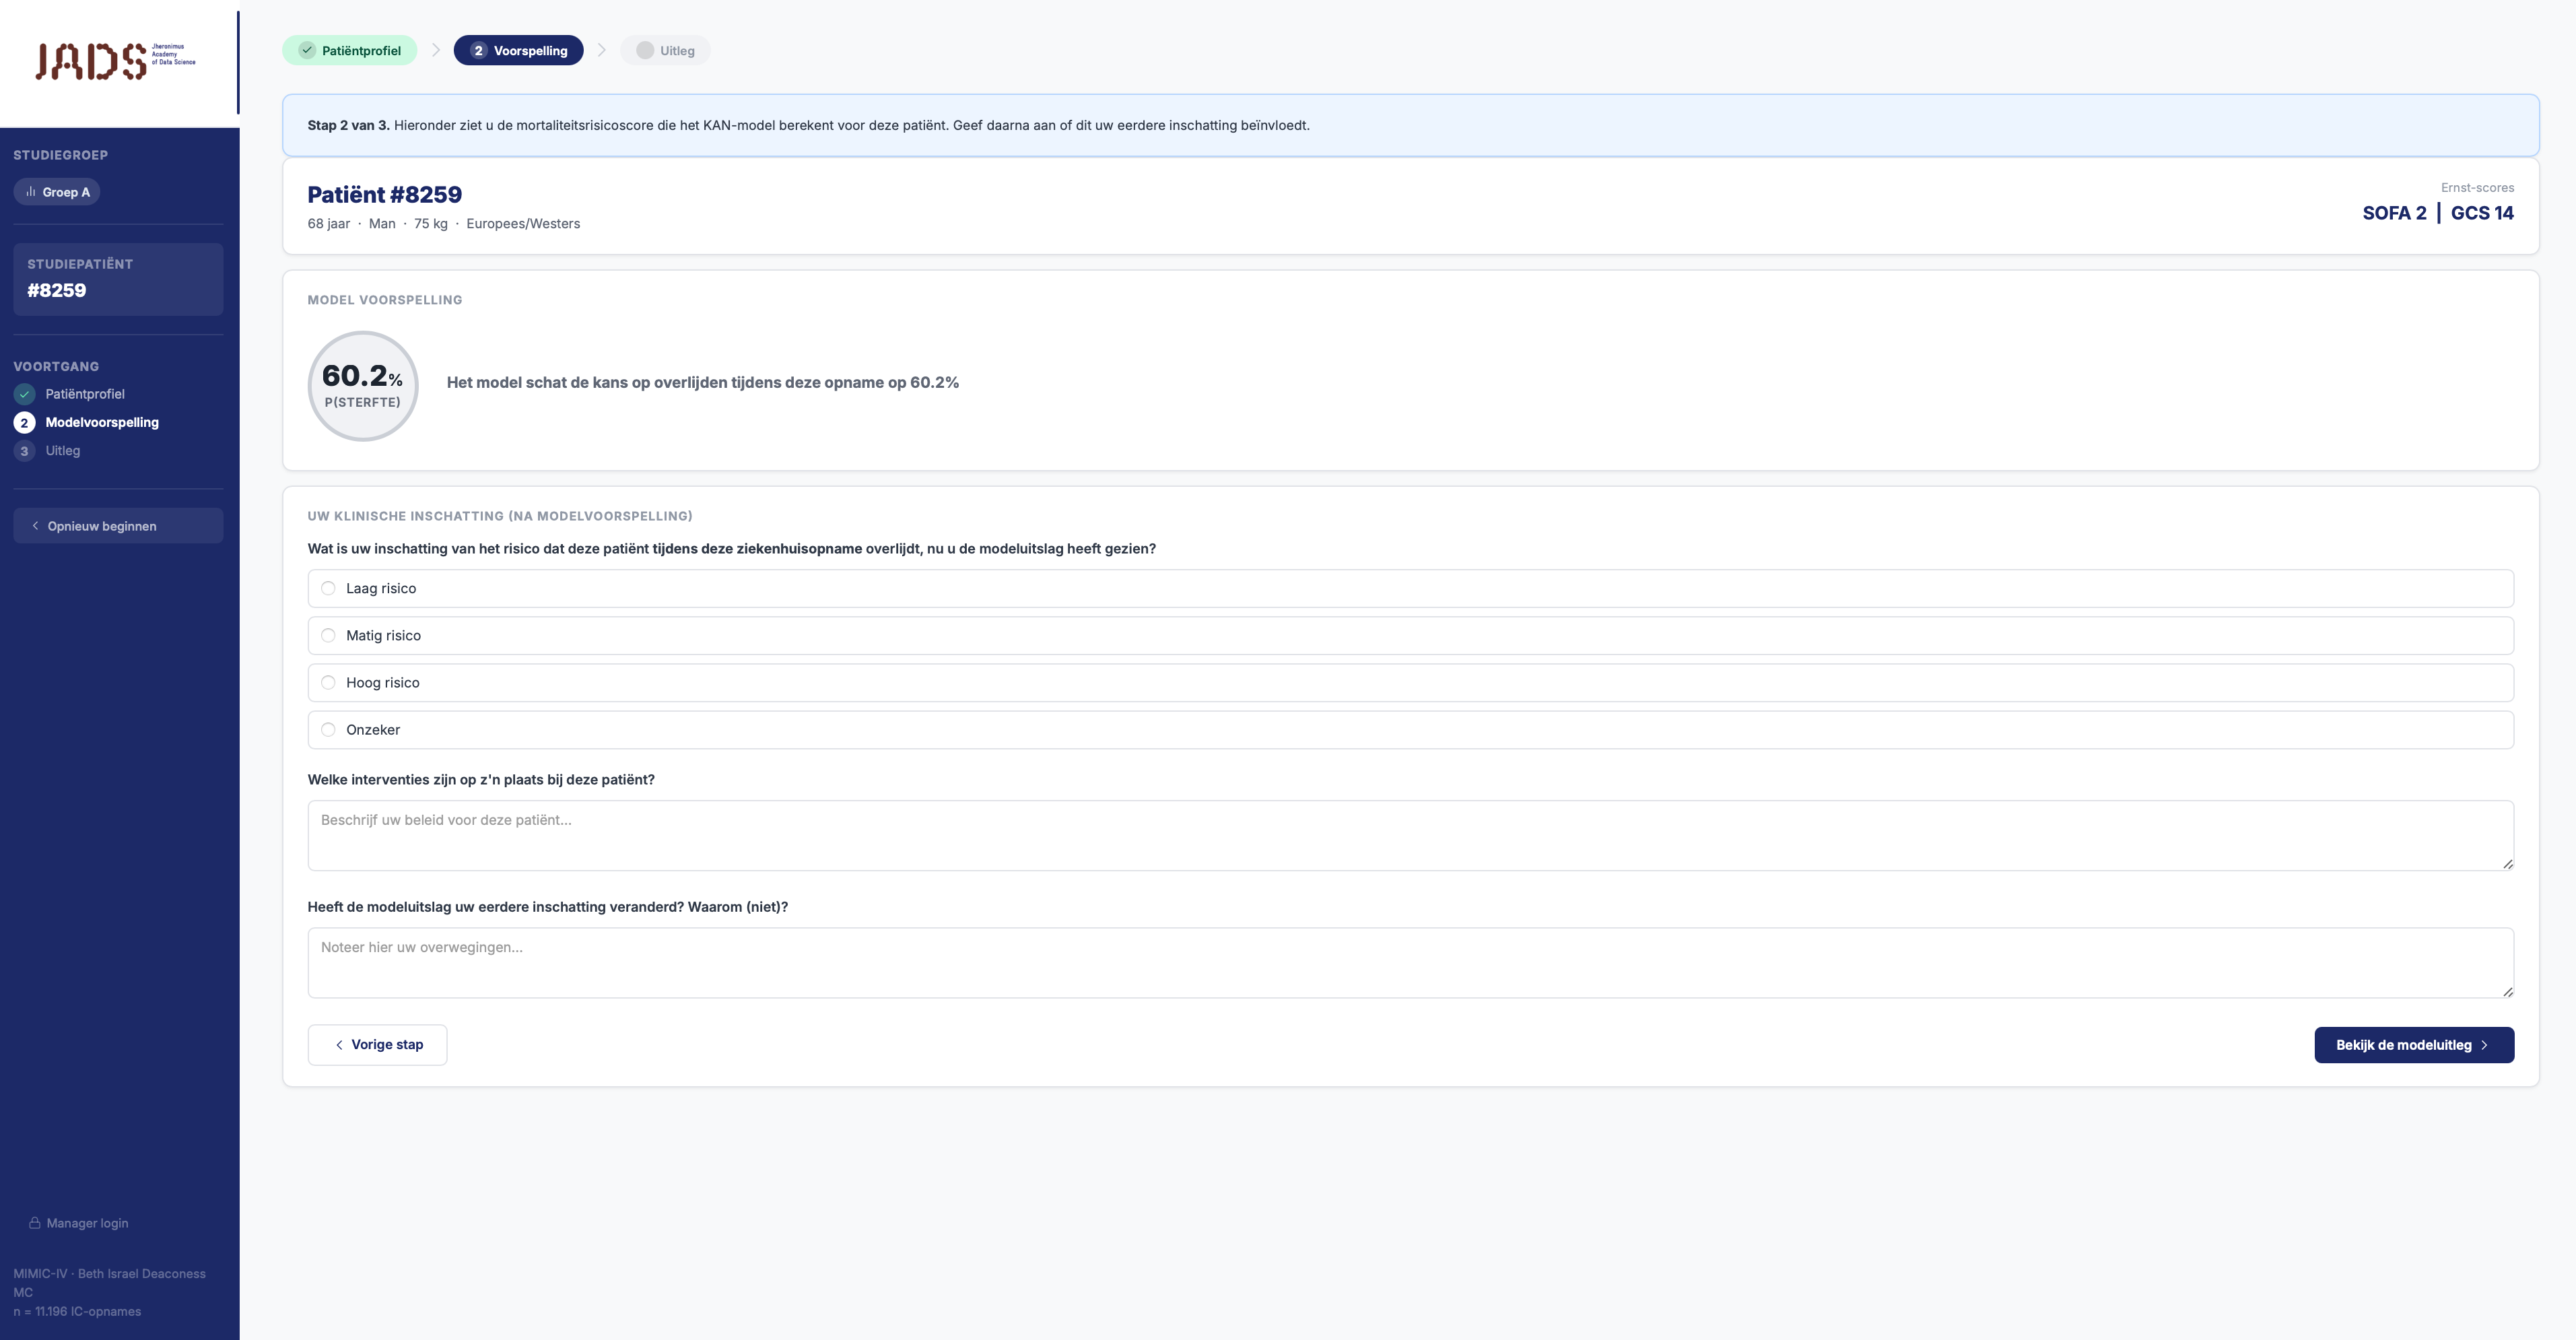
\includegraphics[width=\textwidth]{SupplementaryImages/screen2.png}
  \caption[Step~2: Model prediction]{Step~2: The KAN model's predicted
    in-hospital mortality probability (60.2\%, elevated) is displayed.}
  \label{fig:screen2}
\end{figure}

\noindent\textit{Translation (screen2):}

\smallskip\noindent\textit{Banner:} ``Step 2 of 3: Below you will find the
mortality risk score calculated by the KAN model for this patient. Indicate
whether this influences your further assessment.''

\smallskip\noindent\textbf{Model prediction:} ``The model estimates the
probability of dying during this admission at 60.2\%''

\smallskip\noindent\textsc{Your clinical assessment (after model prediction)}

\smallskip\noindent\textbf{(Q1)} What is your assessment of the risk that
this patient will die during this hospital admission, now that you have seen
the model output?
\emph{(Low risk / Moderate risk / High risk / Uncertain)}

\smallskip\noindent\textbf{(Q2)} What interventions are appropriate for
this patient?

\smallskip\noindent\textbf{(Q3)} Has the model output changed your further
assessment? Why (not)?

% ── Screen 4a: Explanation charts, Group A ────────────────────────────────────
\clearpage
\begin{figure}[htbp]
  \centering
  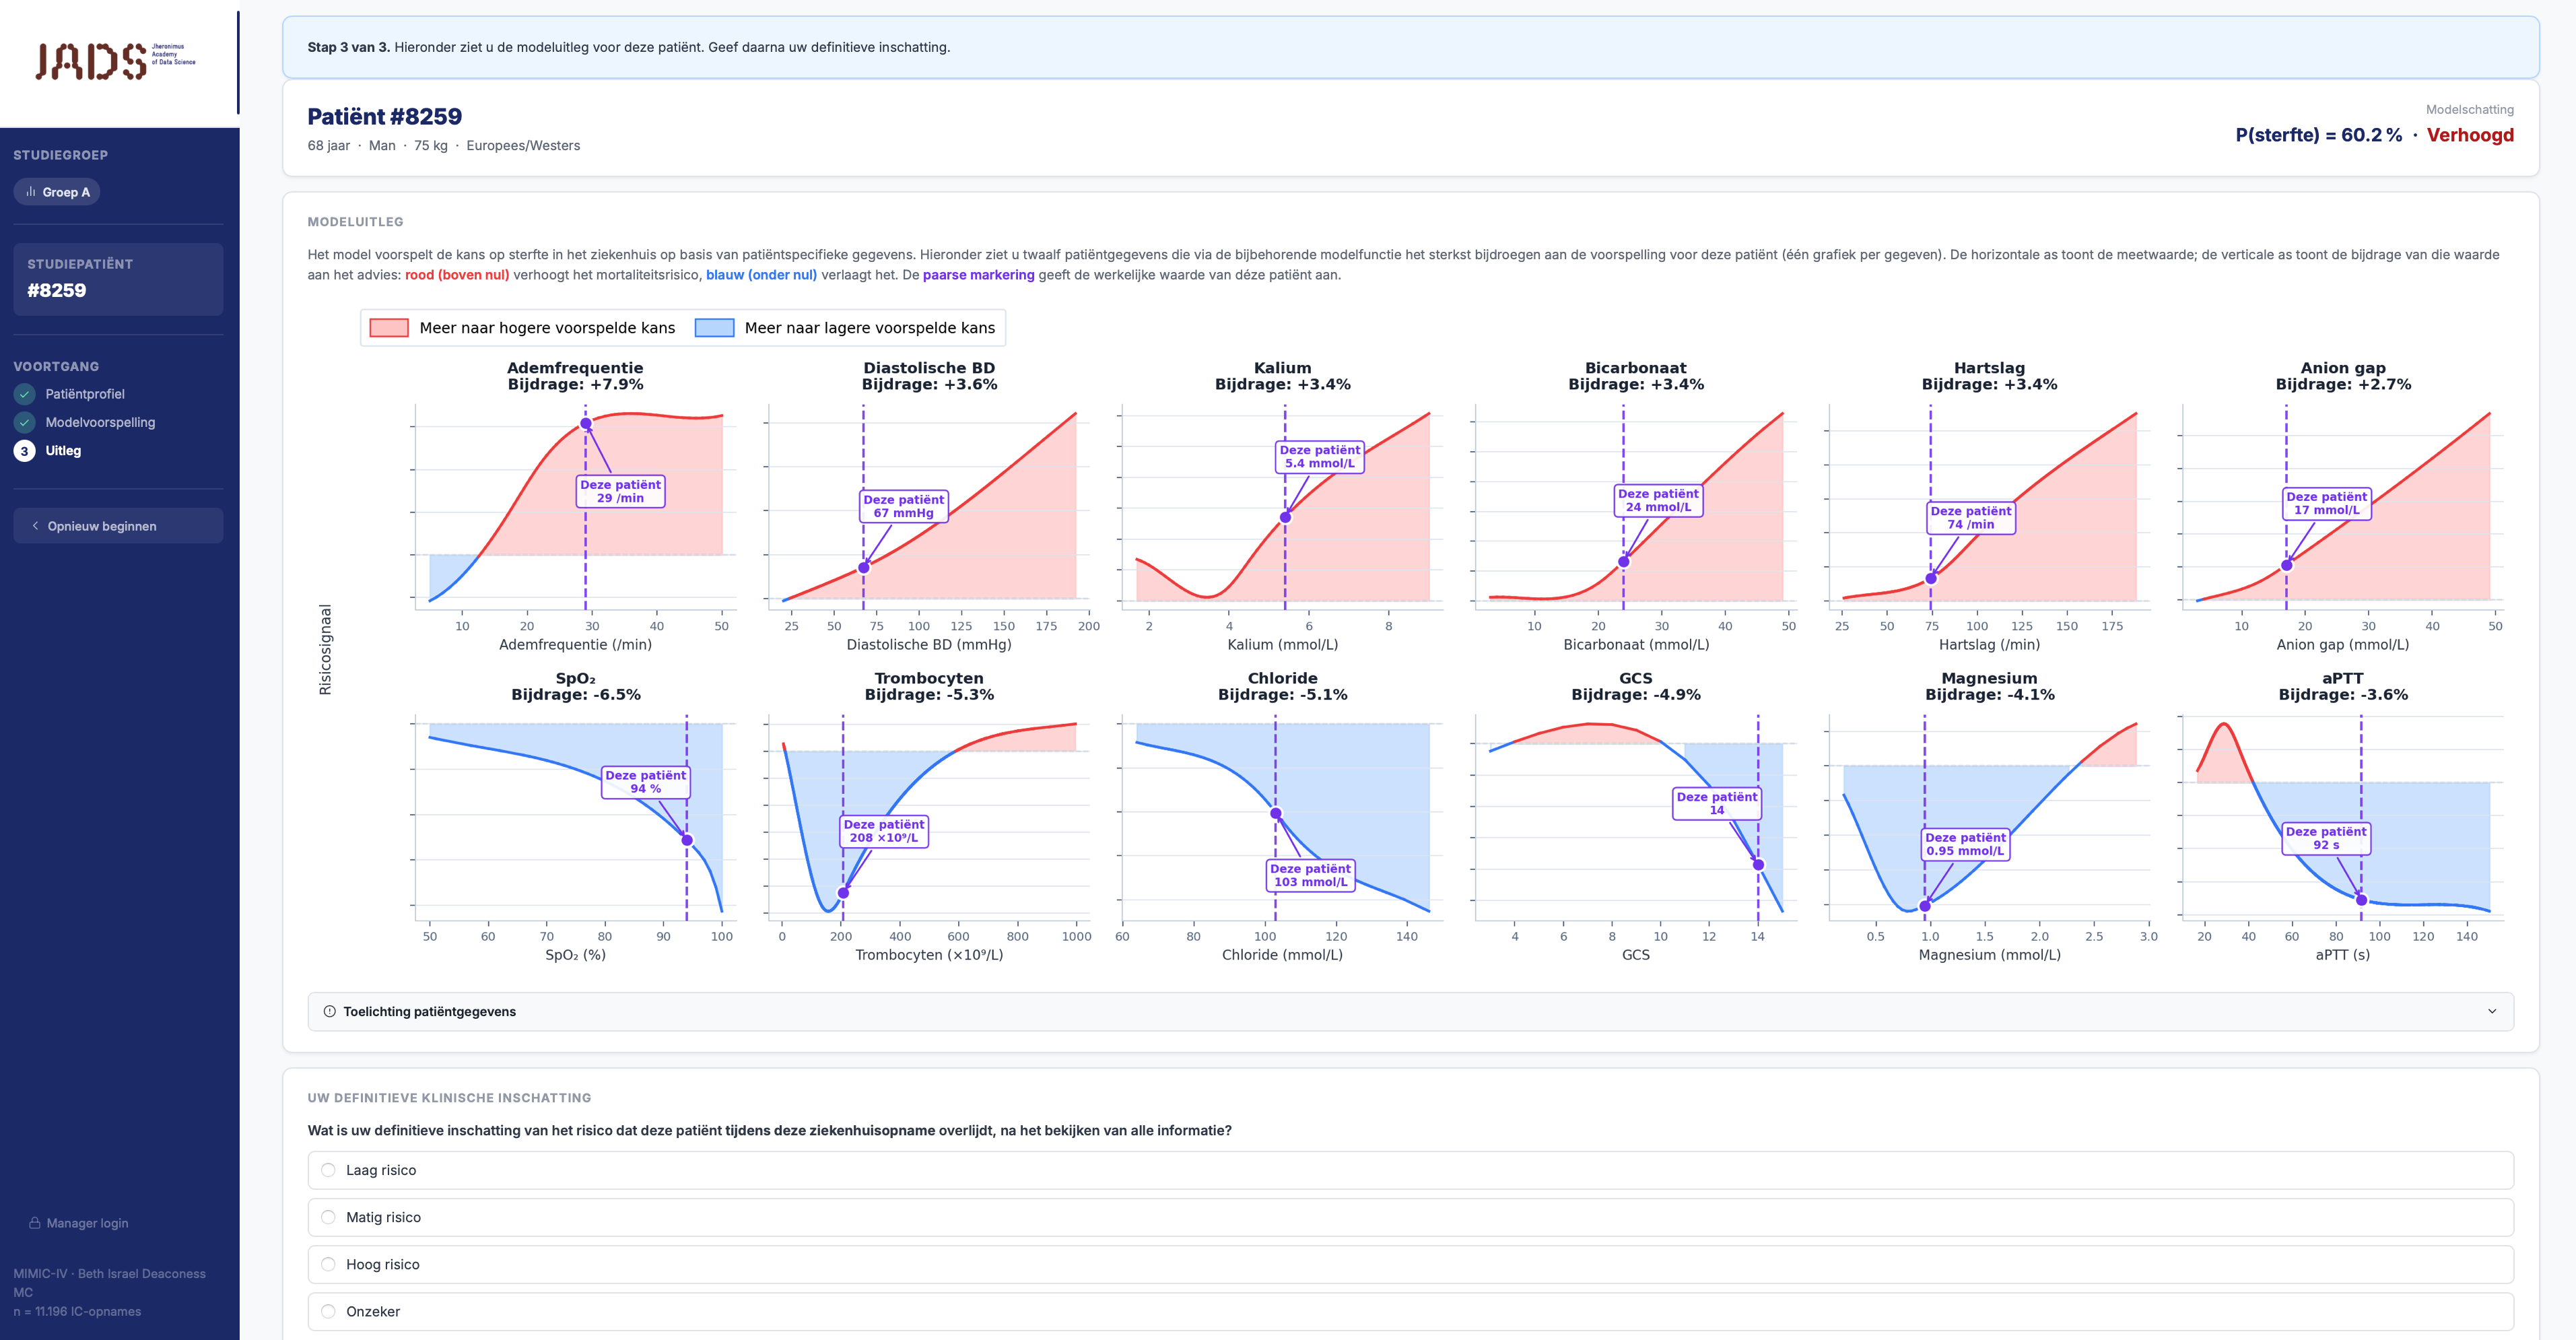
\includegraphics[width=\textwidth]{SupplementaryImages/screen3_A_1.png}
  \caption[Step~3 Group~A part~1: Charts]{Step~3, Group~A (charts only),
    part~1: Twelve spline-based feature-contribution charts.}
  \label{fig:screen3a1}
\end{figure}

\noindent\textit{Translation (screen3\_A\_1):}

\smallskip\noindent\textit{Banner:} ``Step 3 of 3: Below you will find the
model explanation for this patient. Then give your definitive assessment.''

\smallskip\noindent\textit{Chart description:} ``The model predicts the
probability of in-hospital death based on patient-specific data. Below you
can see twelve patient data points that, via the associated model function,
contribute most strongly to the prediction for this patient (one chart per
feature). The horizontal axis shows the measured value; the vertical axis
shows the contribution of that value to the prediction: \textcolor{red}{red
(above zero)} increases the mortality risk, \textcolor{blue}{blue (below
zero)} decreases it. The \textcolor{violet}{purple} marker indicates the
patient's actual value.''

\smallskip\noindent\textit{Legend:} Red = ``More towards higher predicted
probability'' \textbar{} Blue = ``More towards lower predicted probability''

\smallskip\noindent\textsc{Your definitive clinical assessment (begins here, continued on next screen)}

\smallskip\noindent\textbf{(Q1)} What is your definitive assessment of the
risk that this patient will die during this hospital admission, after
viewing all information?
\emph{(Low risk / Moderate risk / High risk / Uncertain)}

% ── Screen 5a: Final assessment + CAS, Group A ───────────────────────────────
\clearpage
\begin{figure}[htbp]
  \centering
  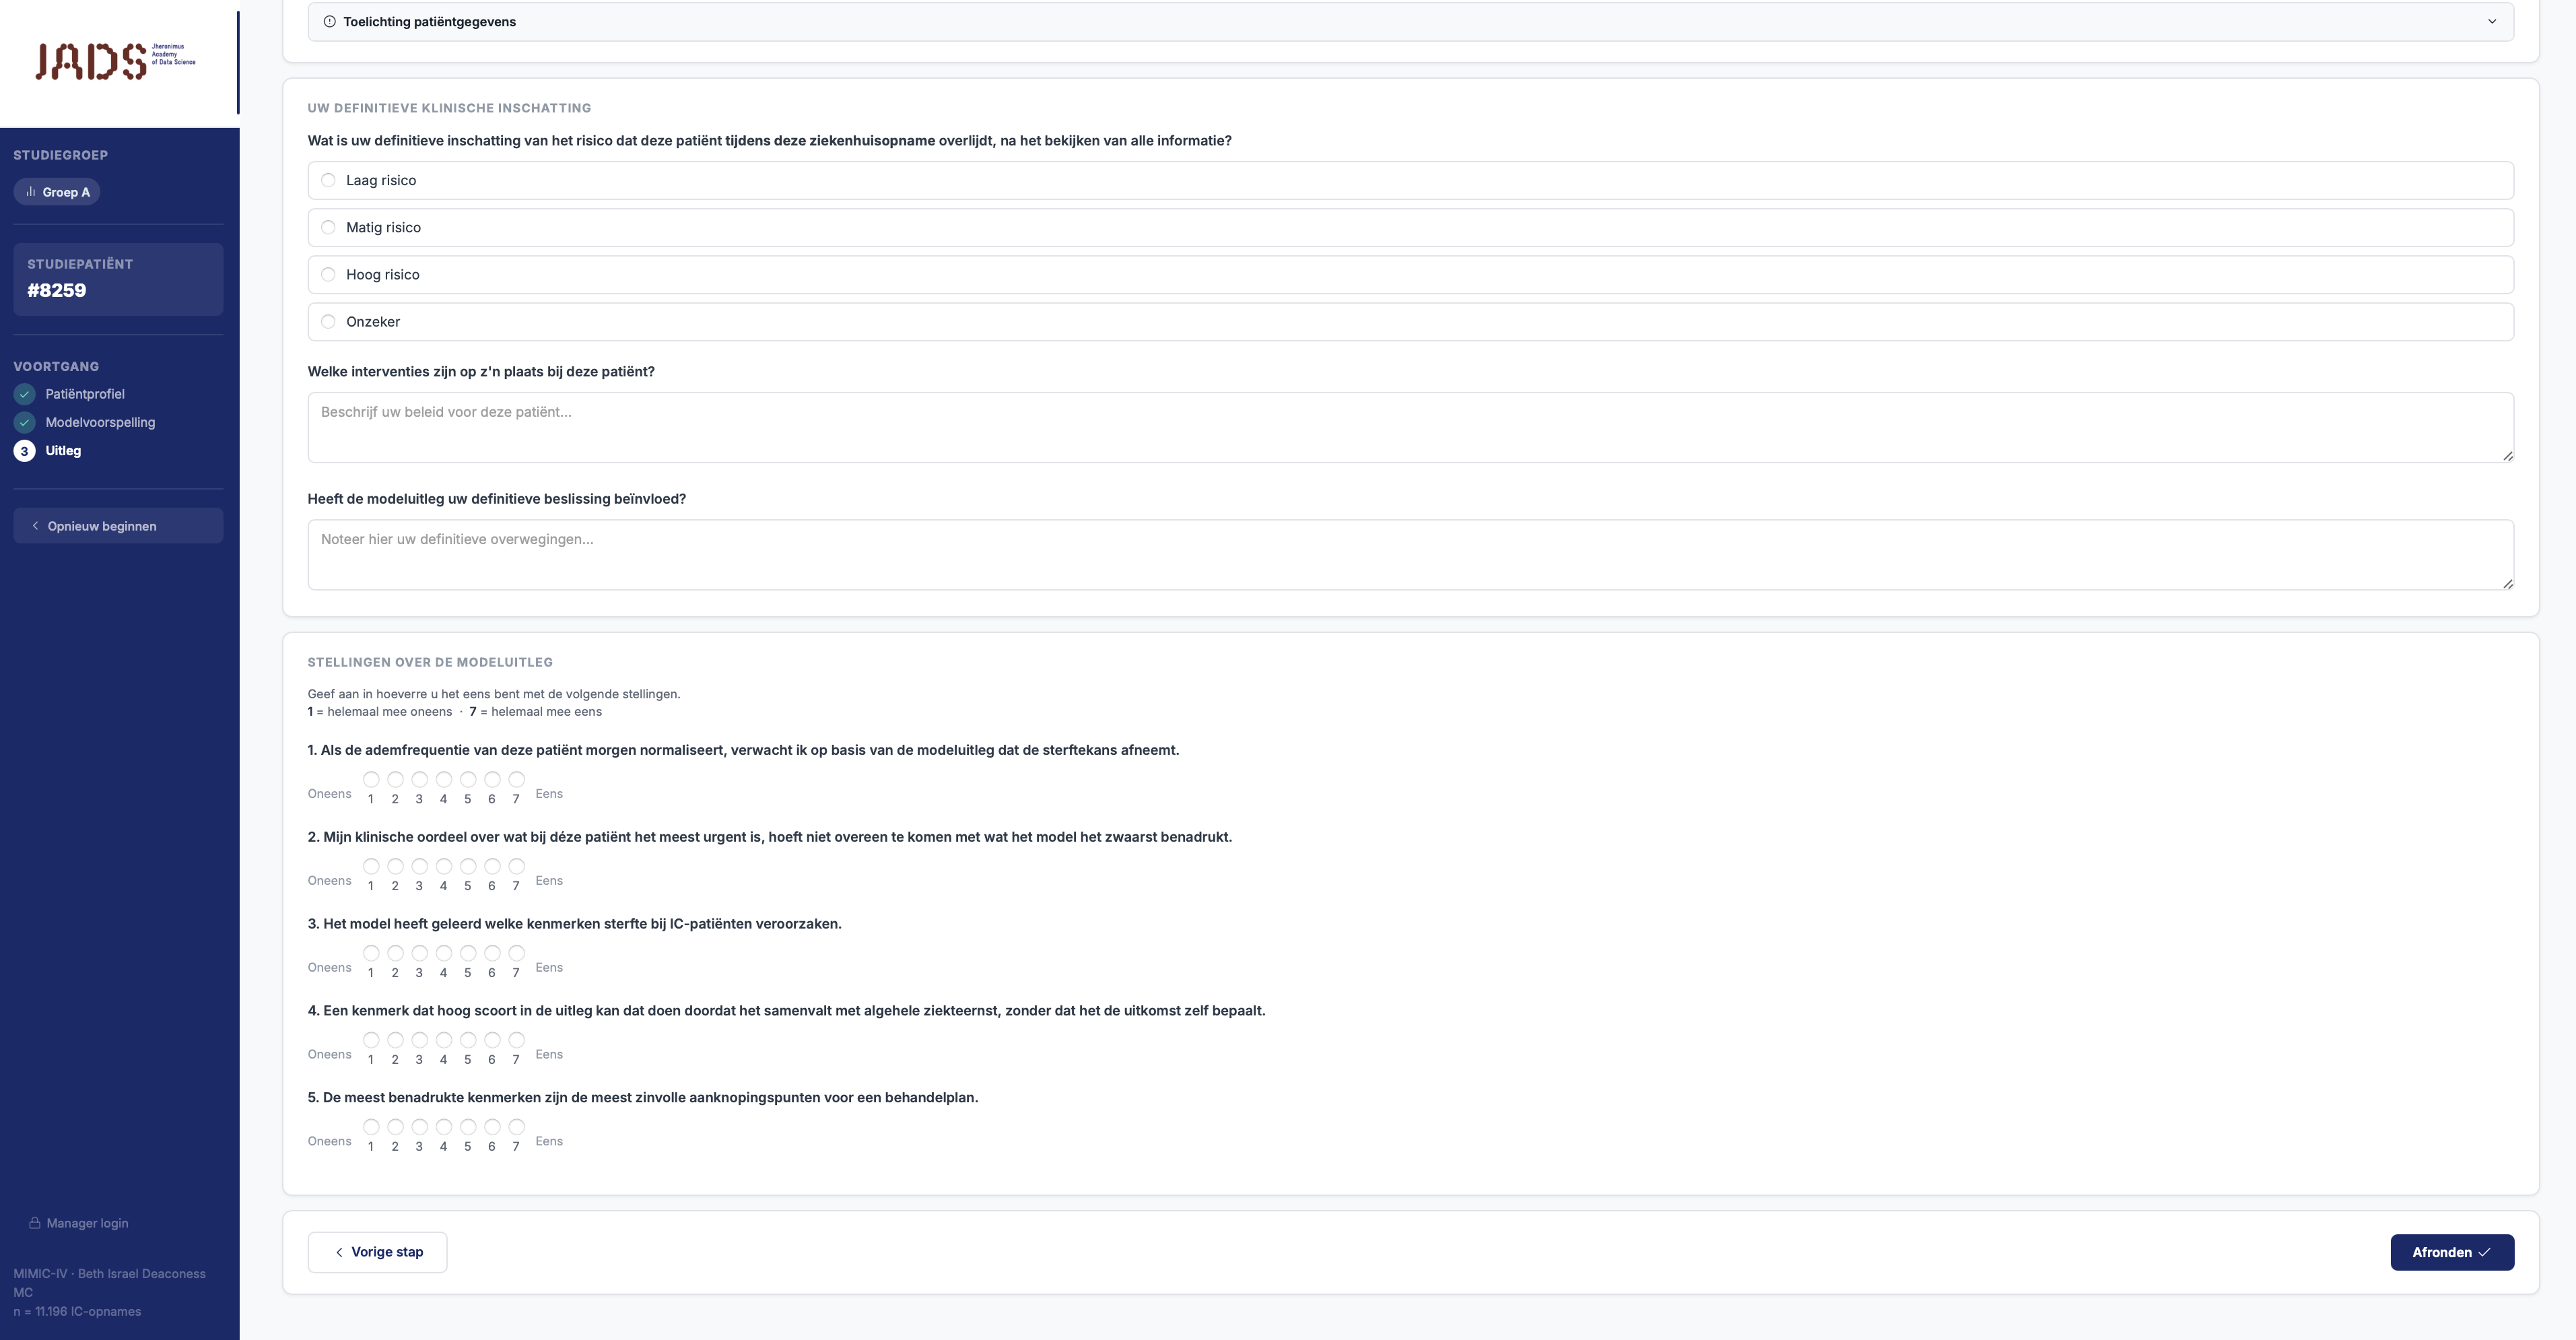
\includegraphics[width=\textwidth]{SupplementaryImages/screen3_A_2.png}
  \caption[Step~3 Group~A part~2: Final assessment + CAS]{Step~3,
    Group~A (charts only), part~2: Definitive assessment and five-item
    Causal Attribution Scale.}
  \label{fig:screen3a2}
\end{figure}

\noindent\textit{Translation (screen3\_A\_2):}

\smallskip\noindent\textsc{Your definitive clinical assessment (continued)}

\smallskip\noindent\textbf{(Q1} cont.) \emph{Low risk / Moderate risk /
High risk / Uncertain}

\smallskip\noindent\textbf{(Q2)} What interventions are appropriate for
this patient?

\smallskip\noindent\textbf{(Q3)} Has the model output influenced your
definitive decision?

\smallskip\noindent\textsc{Statements about the model explanation}

\smallskip\noindent\textit{Instruction:} ``Indicate to what extent you
agree with the following statements. 1 = totally disagree / 7 = totally
agree.''

\smallskip
\begin{enumerate}
  \item ``If this patient's respiratory rate normalises tomorrow, I expect,
    based on the model explanation, that the mortality probability will
    decrease.''
  \item ``My clinical judgement about what is most urgent for this patient
    does not need to correspond with what the model emphasises most.''
  \item ``The model has learned which features cause mortality in ICU
    patients.''
  \item ``A feature that scores highly in the explanation can do so because
    it co-occurs with overall illness severity, without itself determining
    the outcome.''
  \item ``The most emphasised features are the most clinically relevant
    starting points for a treatment plan.''
\end{enumerate}

% ── Screen 4b: Explanation charts + LLM narrative, Group B ───────────────────
\clearpage
\begin{figure}[htbp]
  \centering
  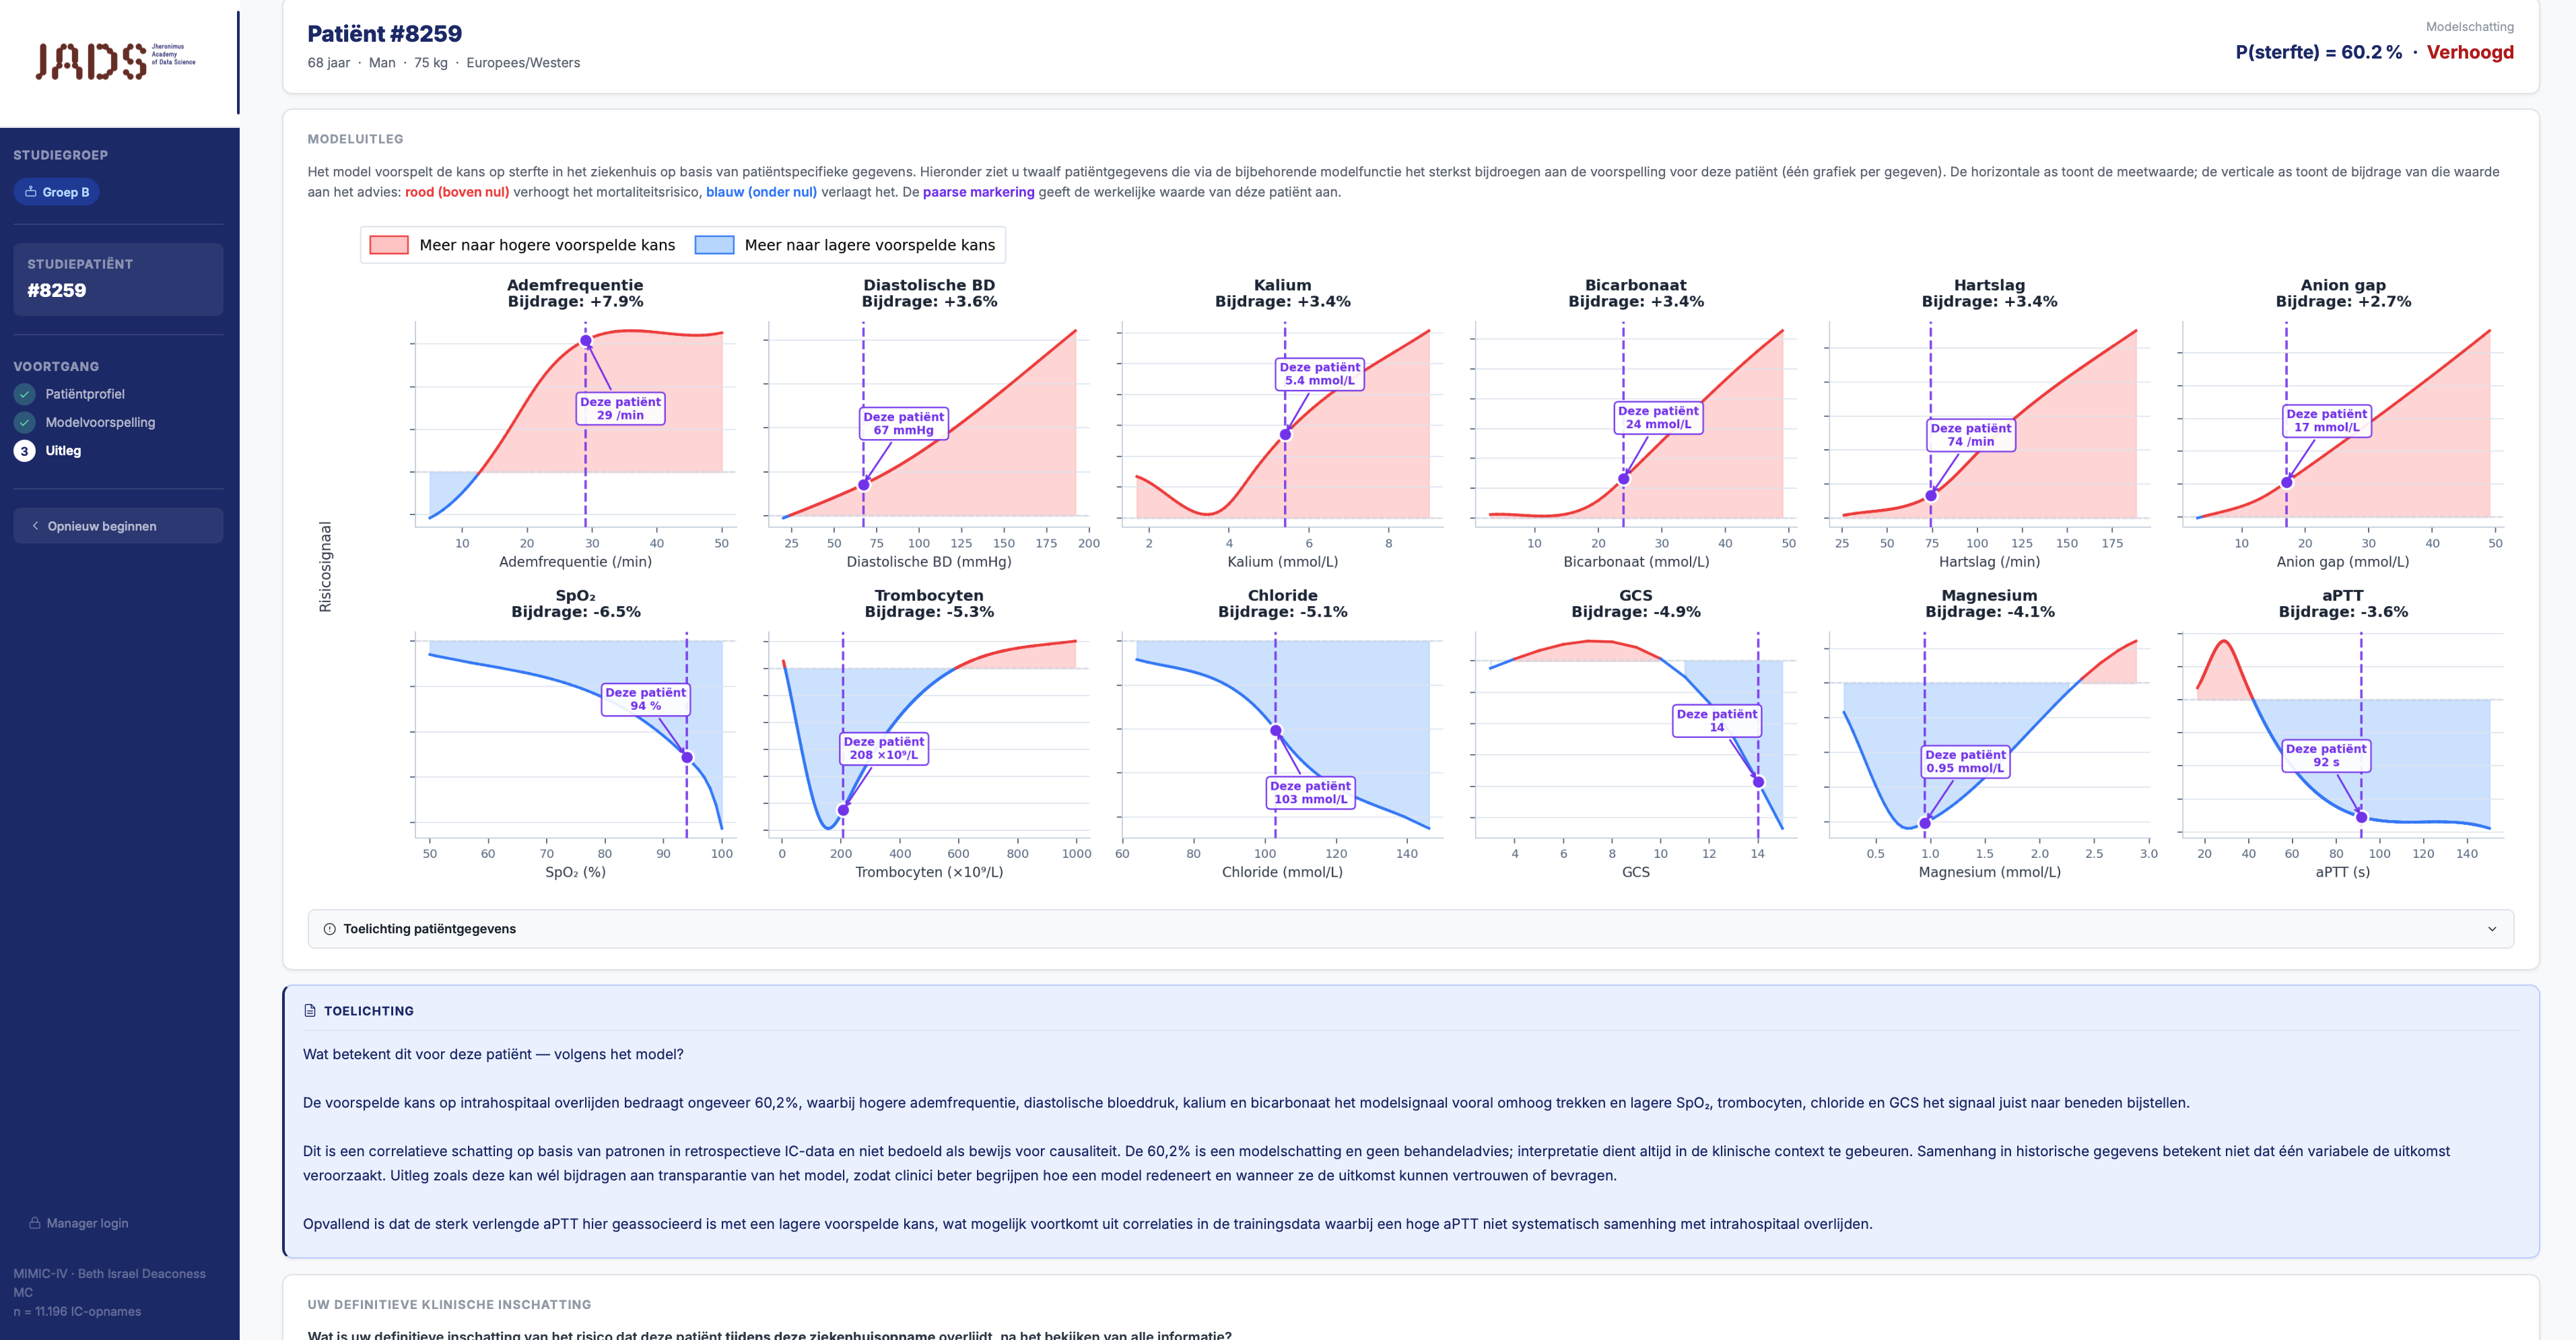
\includegraphics[width=\textwidth]{SupplementaryImages/screen3_B_1.png}
  \caption[Step~3 Group~B part~1: Charts + LLM narrative]{Step~3,
    Group~B (charts + LLM narrative), part~1: Identical charts as
    Group~A, with an LLM-generated explanation (\emph{Toelichting})
    appended below.}
  \label{fig:screen3b1}
\end{figure}

\noindent\textit{Translation of LLM narrative (screen3\_B\_1 ---
\emph{Toelichting} section):}

\smallskip\noindent\textbf{What does this mean for this patient ---
according to the model?}

\smallskip\noindent The predicted probability of in-hospital death is
approximately 60.2\%, with higher respiratory rate, diastolic blood
pressure, potassium and bicarbonate primarily pulling the model signal
upward, while lower SpO$_2$, platelets, chloride and GCS pull the signal
slightly downward.

\smallskip\noindent This is a correlational estimate based on patterns in
retrospective ICU data and is not intended as evidence of causality. The
60.2\% is a model estimate and not treatment advice; interpretation should
always occur in the clinical context. Associations in historical data do
not mean that one variable causes the outcome. Explanations such as these
can contribute to the transparency of the model, so that clinicians better
understand how a model reasons and when they can trust or question the
outcome.

\smallskip\noindent It is notable that the markedly elevated aPTT here is
associated with a lower predicted probability, which may stem from
correlations in the training data in which a high aPTT does not
systematically co-occur with in-hospital death.

% ── Screen 5b: Final assessment + CAS, Group B ───────────────────────────────
\clearpage
\begin{figure}[htbp]
  \centering
  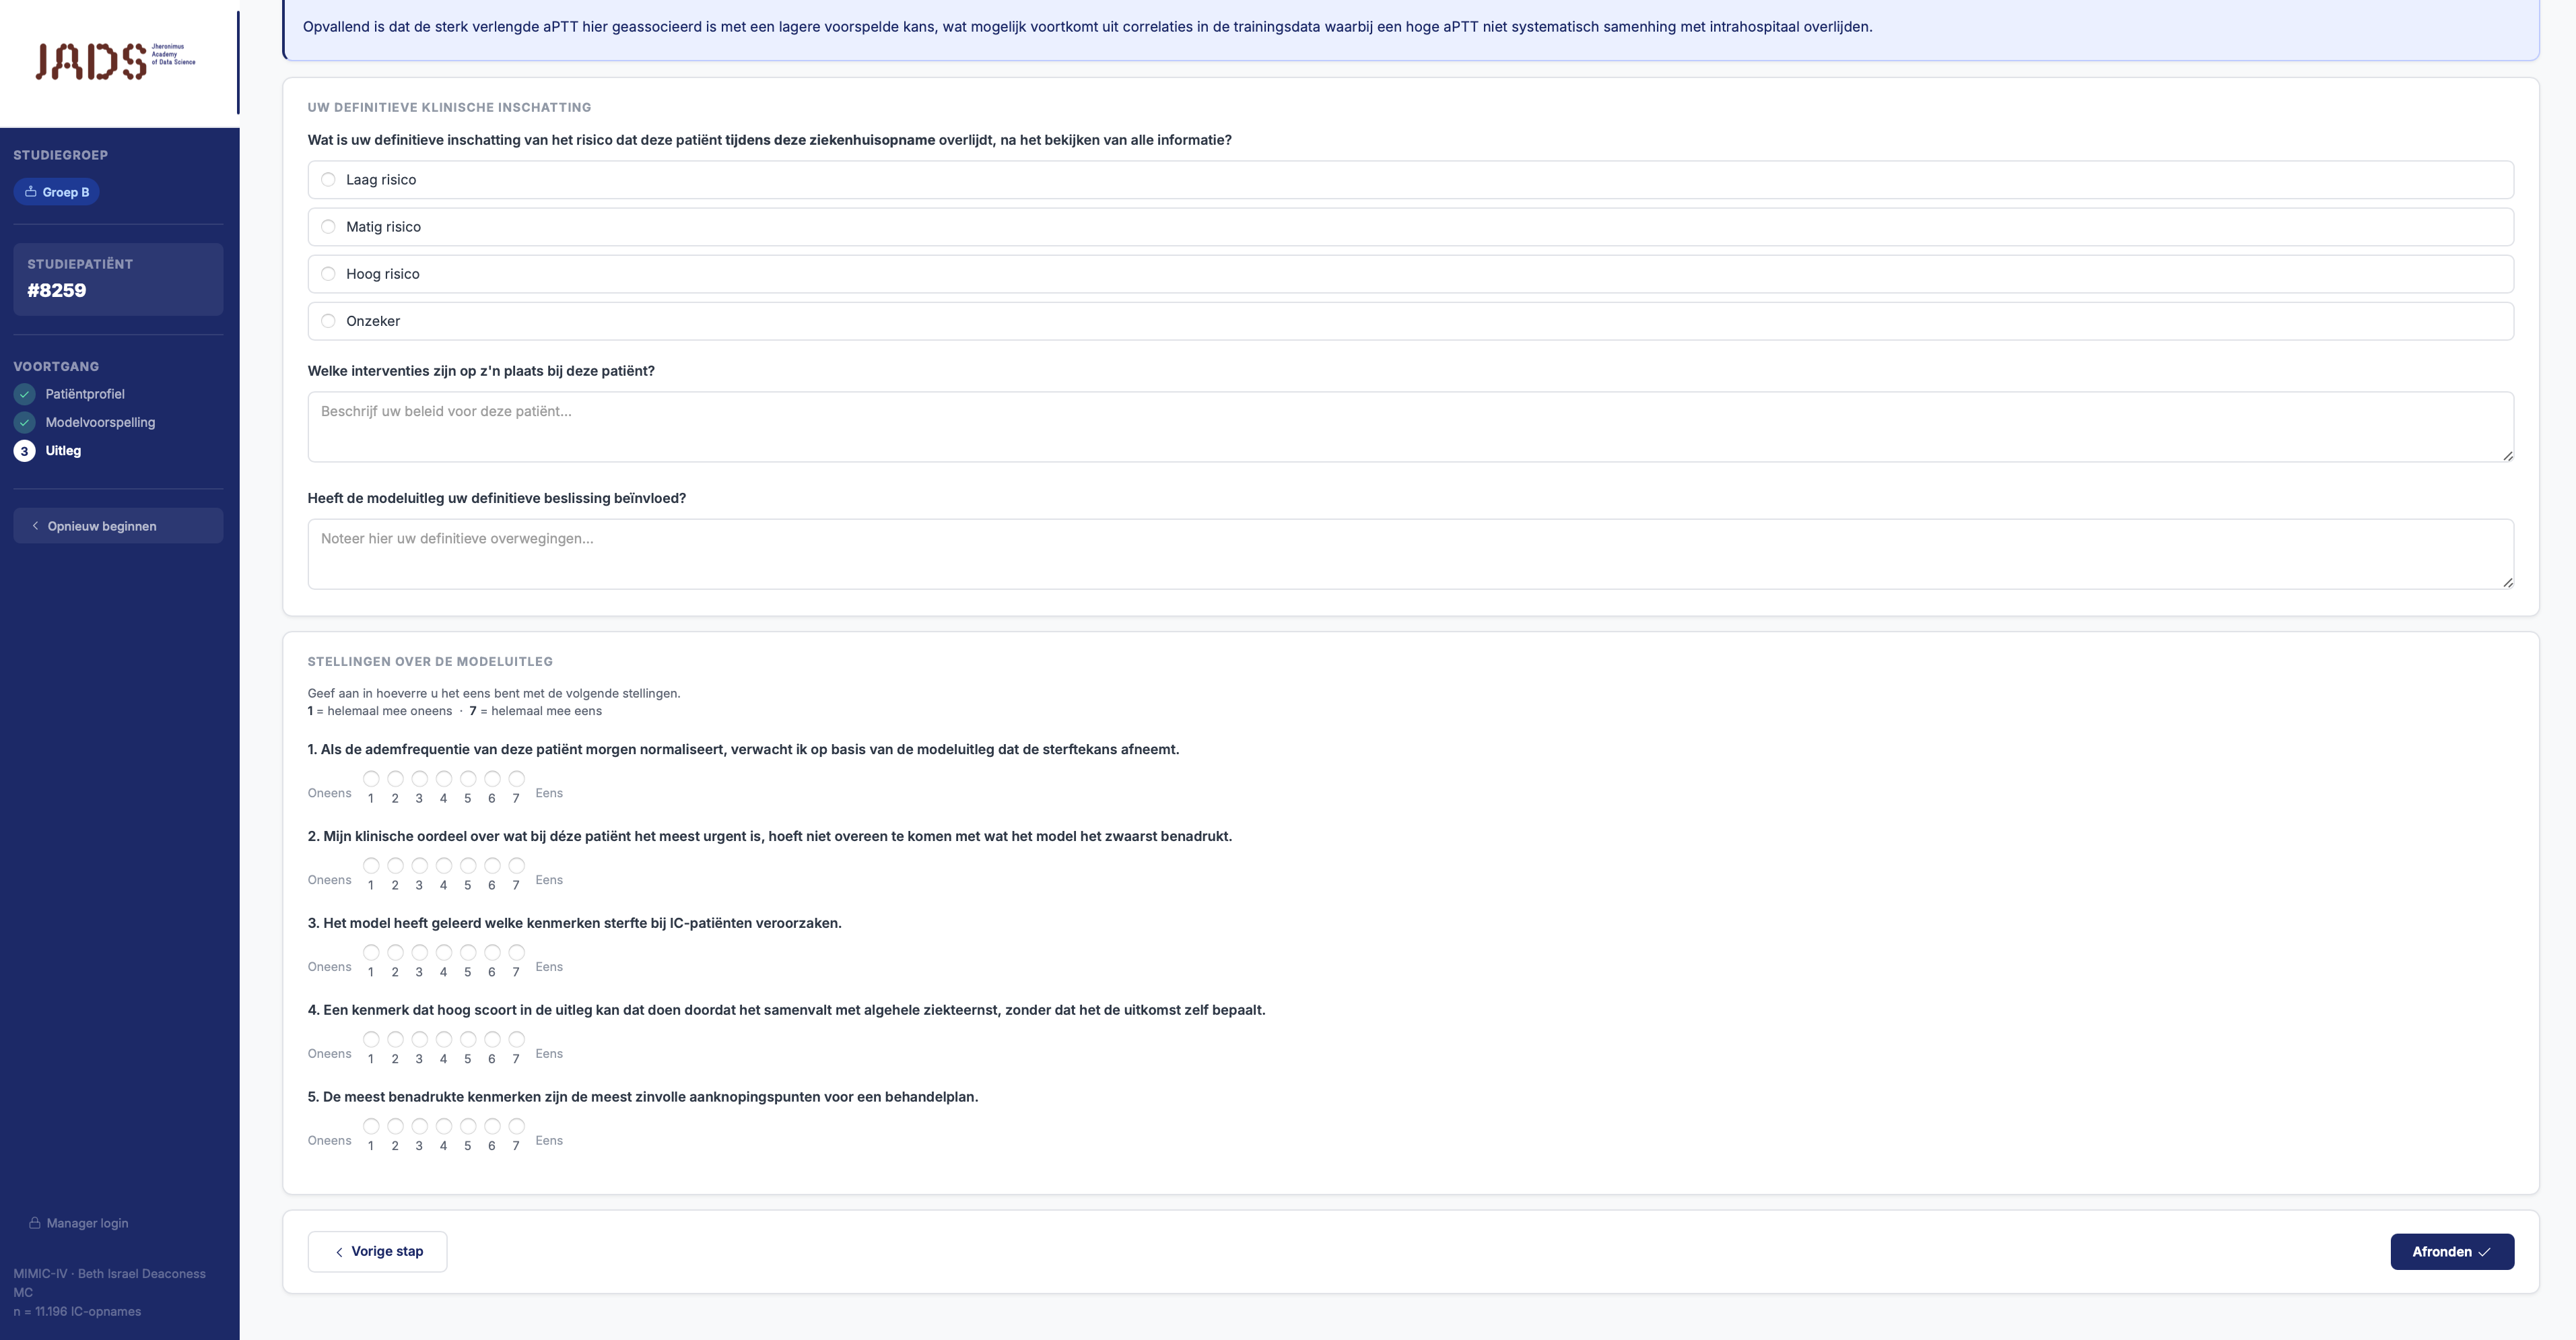
\includegraphics[width=\textwidth]{SupplementaryImages/screen3_B_2.png}
  \caption[Step~3 Group~B part~2: Final assessment + CAS]{Step~3,
    Group~B (charts + LLM narrative), part~2: Definitive assessment and
    Causal Attribution Scale, identical in structure to
    Group~A (Figure~\ref{fig:screen3a2}).}
  \label{fig:screen3b2}
\end{figure}

\noindent\textit{(Translation identical to screen3\_A\_2 above.)}

% ── Appendix: Co-12 pre-study validation ─────────────────────────────────────
\clearpage
\section{Co-12 Pre-study Validation Outputs}
\label{app:co12_prestudy}

Outputs for Consistency (ten baseline generations) and Continuity (one
perturbed regeneration). Perturbation mode was enabled with a
KAN forward pass on slightly altered inputs. The LLM produced Dutch text for
participants; English translations of the stored outputs are given below.

\subsection*{Consistency --- ten independent generations}

% English translation of 10xgeneration.txt (Dutch outputs shown to participants)
\begin{quote}\footnotesize
LLM responses --- ten generations

Response 1\\
What does this mean for this patient --- according to the model?

The predicted probability of in-hospital mortality for this patient is approximately 60.2\%. The model signal is pulled up mainly by elevated respiratory rate, diastolic blood pressure, potassium, and bicarbonate, while SpO\textsubscript{2}, platelets, chloride, and GCS pull the signal down.

This estimate is based on correlations in historical ICU data and says nothing about causality. The figure of 60.2\% is a model estimate, not treatment advice. Interpretation must always occur in clinical context, because association in retrospective data does not imply a causal link. Clinical judgement and patient-specific details remain crucial. Explanation of this type can help make the model transparent so clinicians better understand how a model reasons and when to trust or challenge the output.

It stands out that a markedly prolonged aPTT---clearly above the reference value---contributes to lower predicted probability. Such patterns can arise when rare values in the training data occurred mainly in subgroups with relatively favourable outcomes, or through selection bias in retrospectively collected data.

Response 2\\
What does this mean for this patient --- according to the model?

The predicted probability of in-hospital mortality is 60.2\%, with higher respiratory rate, diastolic blood pressure, potassium, and bicarbonate pulling the model signal up, and lower oxygen saturation, platelet count, chloride, and GCS score pulling it down.

This is a purely correlational estimate based on patterns in historical ICU data and is not evidence that a specific measurement causes the outcome. The 60.2\% is a model estimate and not treatment advice. Interpretation should always occur in clinical context; association in retrospective data is no guarantee of causality. Such explanation contributes to transparency of machine learning models so clinicians can better understand how the model reasons and when the output is reliable or warrants further scrutiny.

It stands out that a prolonged aPTT above reference values is associated with lower predicted mortality. This pattern may follow from confounders in retrospective data, for example because patients with a prolonged coagulation profile received more intensive monitoring or treatment. It indicates that individual measurements, seen in isolation, can sometimes contribute counter-intuitively to the model signal.

Response 3\\
What does this mean for this patient --- according to the model?

The predicted probability of in-hospital mortality is 60.2\%, and the model signal is pulled up mainly by elevated respiratory rate, diastolic blood pressure, potassium, and bicarbonate, while lower SpO\textsubscript{2}, platelet count, chloride, and GCS pull the signal down.

This is a correlational estimate based on patterns from historical ICU data and is not intended as evidence of a cause--effect relation. The 60.2\% is a model estimate and not treatment advice. Interpretation should always occur in clinical context, because association in retrospective data does not automatically indicate causality. Clinical assessment and additional diagnostics remain indispensable. Explanation of this type of model can however help make machine learning predictions transparent so you can better judge when to trust the output or question it further.

A striking pattern is that the markedly prolonged aPTT, although above reference, contributes to lower predicted mortality. This may follow from retrospective correlations in which patients with such aPTT prolongation underwent fewer acute resuscitations or invasive procedures under certain circumstances. Such associations illustrate the importance of viewing all features jointly rather than in isolation.

Response 4\\
What does this mean for this patient --- according to the model?

The predicted probability of in-hospital mortality is 60.2\% according to the model. Respiratory rate, diastolic blood pressure, potassium, and bicarbonate pull the model signal up mainly, while SpO\textsubscript{2}, platelets, chloride, and GCS pull the signal down.

This is a correlational estimate based on patterns in historical ICU data and is not intended as proof that one measurement directly causes the outcome. The 60.2\% is a model estimate and not treatment advice. Interpretation of this output must always occur in the clinical context of the individual patient. Association in retrospective data does not imply causality and may be influenced by unobserved factors. This type of explanation helps make machine learning models transparent so clinicians understand how a model reasons and when to trust or critically question the output.

The model associates a markedly prolonged aPTT above reference with lower predicted mortality, which is not directly clinically intuitive. This pattern may follow from retrospective correlations in which patients with prolonged aPTT in the training data may have had less acute mortality risk or fell under specific treatment protocols.

Response 5\\
What does this mean for this patient --- according to the model?

The predicted probability of in-hospital mortality is approximately 60.2\%. The model signal is pulled up mainly by high respiratory rate, relatively low diastolic blood pressure, elevated potassium and bicarbonate values, while lower oxygen saturation, normal platelets, chloride, and a near-maximal GCS score pull the predicted probability down.

This is a correlational estimate based on historical ICU data and offers no proof that one measurement causes the outcome. The value of 60.2\% is a model output and not treatment advice. Interpretation must always occur within clinical context and alongside other clinical judgement, because association in retrospective data does not imply causality. This model result can give insight into factors an algorithm uses, but does not replace medical decision-making. With this type of explanation clinicians can better understand how a model reasons and judge when to trust or critically question the output.

A striking pattern is that a markedly prolonged aPTT, although above reference, is linked by the model to lower predicted mortality. This may reflect a retrospective association in which patients with coagulation abnormalities in the training data received more intensive monitoring or treatment, giving this feature an opposite contribution.

Response 6\\
What does this mean for this patient --- according to the model?

The predicted probability of in-hospital mortality for this admission is 60.2\%, with higher respiratory rate, diastolic blood pressure, potassium, and bicarbonate pulling the risk signal up and lower SpO\textsubscript{2}, platelets, chloride, and GCS pulling the signal down.

This is a correlational estimate based on patterns in historical ICU data and offers no evidence of cause and effect. The 60.2\% is a model estimate and not treatment advice. Interpretation should always occur in clinical context and account for all available patient data. Association in retrospective data does not imply that a single measurement causes the outcome. This type of explanation is especially valuable for making machine learning models transparent so clinicians understand how a model reasons and when to trust or critically question the output.

It is possible that a markedly prolonged aPTT---above the reference range---contributes to lower predicted probability. Such patterns can arise in retrospective data when certain patient subgroups with abnormal laboratory values simultaneously show other risk factors.

Response 7\\
What does this mean for this patient --- according to the model?

The predicted probability of in-hospital mortality is 60.2\%. Measurements such as respiratory rate, diastolic blood pressure, potassium, and bicarbonate pull the model signal up mainly, while lower SpO\textsubscript{2}, platelet count, chloride, and GCS pull the signal down.

This estimate is based solely on correlational patterns in historical ICU data and is not evidence that a specific measurement causes the outcome. The 60.2\% is a model estimate and must not be interpreted as treatment advice. Interpretation should always occur in clinical context, accounting for limitations of retrospective data and the absence of causality. It remains essential to combine clinical judgement with this estimate. Explanation like this can help make how the model reasons transparent so clinicians can better judge when to trust or challenge the output.

It stands out that a markedly prolonged aPTT in this model is associated with lower predicted mortality. This pattern can arise from selection bias in the historical data, in which patients with high aPTT values may have had other treatment trajectories or less severe underlying conditions.

Response 8\\
What does this mean for this patient --- according to the model?

The predicted probability of in-hospital mortality is 60.2\%. In this model signal, elevated respiratory rate, diastolic blood pressure, potassium, and bicarbonate pull the probability up mainly, while lower SpO\textsubscript{2}, platelets, chloride, and GCS values pull the signal down.

This estimate is based on correlational patterns in historical ICU data and offers no proof that a single measurement causes the outcome. The value of 60.2\% is a model estimate and not treatment advice. Interpretation must always occur within clinical context, because association in retrospective data is not equivalent to causality. Models like this can contribute to transparency by clarifying which factors weigh in, so clinicians understand how a model reasons and when the output is reliable or warrants further investigation.

It stands out that the aPTT value of 92\,s is clearly above reference but is still involved in lower predicted probability. This may reflect that in the historical data patients with a markedly prolonged aPTT had a different risk profile than expected, for example through heterogeneity in underlying conditions or treatment choices. This emphasises that individual feature contributions must always be judged together with other measurements.

Response 9\\
What does this mean for this patient --- according to the model?

The predicted probability of in-hospital mortality is approximately 60.2\%. Measurements such as respiratory rate, diastolic blood pressure, potassium, and bicarbonate push the model signal up mainly, while lower SpO\textsubscript{2}, platelets, chloride, and GCS pull the signal down.

This is a correlational estimate based on patterns in historical ICU data and is not proof that a specific measurement causes the outcome. The 60.2\% is a model estimate and not treatment advice. Interpretation must always occur in clinical context, because association in retrospective data does not imply causality. Experts should weigh the output against other clinical findings. This form of explanation can help make how the model reasons transparent and when the output is reliable or needs further testing.

It stands out that diastolic blood pressure of 67\,mmHg, although within reference values, still contributes to higher predicted probability. This may follow from correlations in retrospective data in which patients with similar blood pressure values, in combination with other risk factors, had worse outcomes.

Response 10\\
What does this mean for this patient --- according to the model?

The predicted probability of in-hospital mortality for this patient is approximately 60.2\%. Higher respiratory rate, diastolic blood pressure, potassium, and bicarbonate contribute mainly to an increase in this model signal, while the rise in probability is partly offset by relatively normal SpO\textsubscript{2}, platelets, chloride, and GCS values.

This figure is a correlational estimate based on patterns in historical ICU data and offers no proof that a single measurement causes the outcome. It is not treatment advice but an indicative estimate that must always be interpreted in clinical context. Association in retrospective data does not automatically imply causality or direction of effect. This type of explanation can help make the model's logic transparent so clinicians understand how the model reasons and when the output should be assessed or questioned more critically.

It stands out that diastolic blood pressure falls within normal reference values but still pulls the model signal upward. This may follow from confounders in the training data, in which patients with similar pressure values may have had other risk factors associated with poor outcomes.
\end{quote}

\subsection*{Continuity --- perturbed inputs}

\begin{figure}[H]
  \centering
  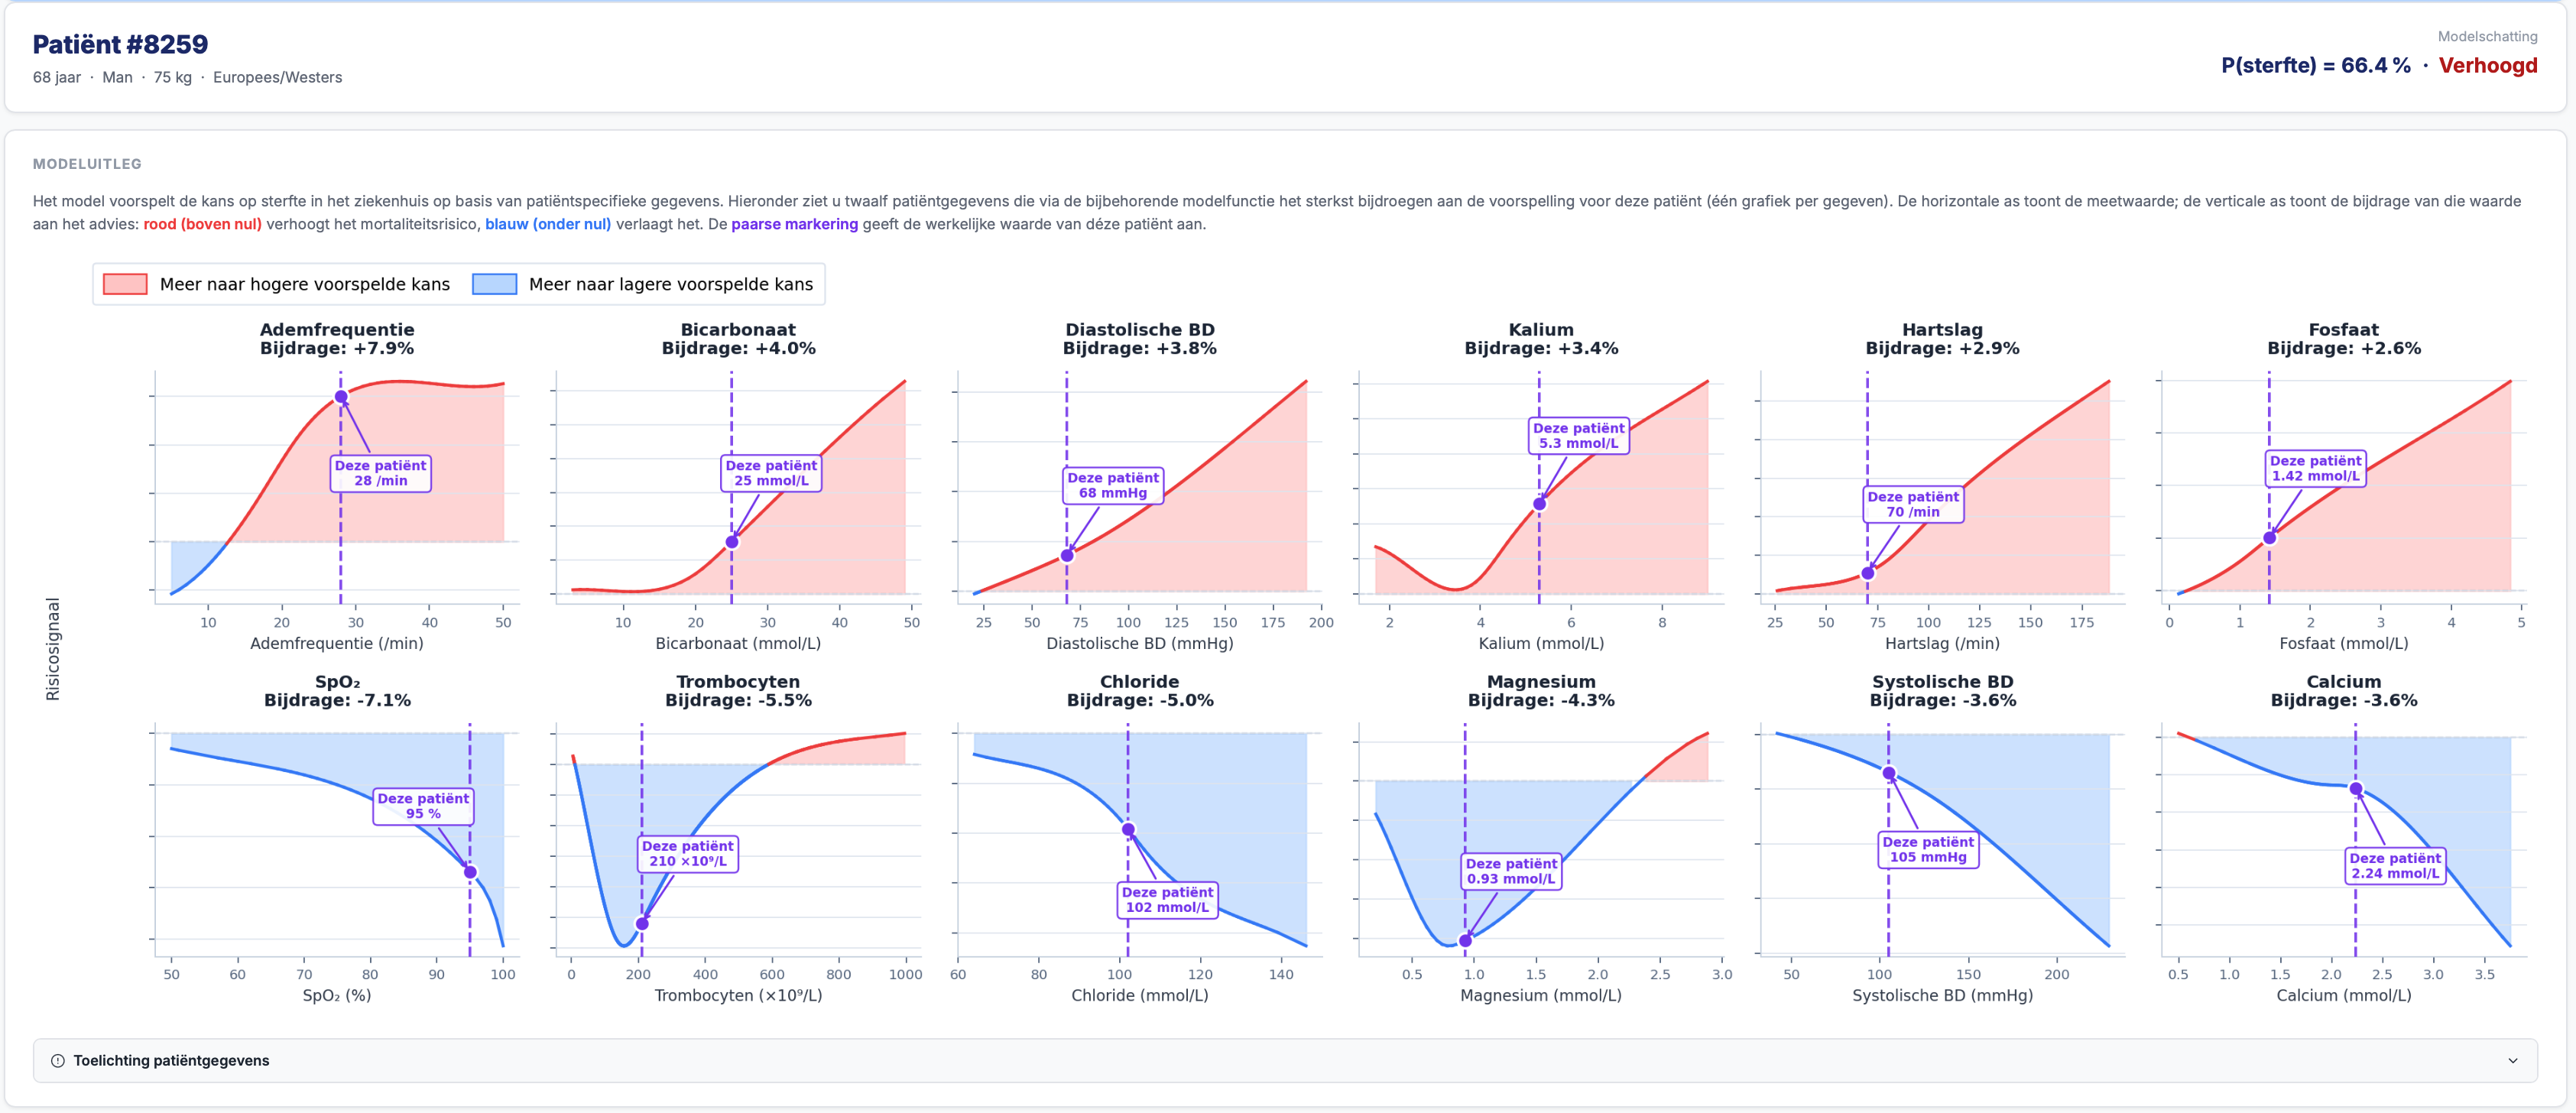
\includegraphics[width=\textwidth]{SupplementaryImages/pertubationSplines.png}
  \caption{Detail panels after input perturbation ($P=66.4\%$).}
  \label{fig:perturbation_splines}
\end{figure}

% English translation of pertubation.txt (Dutch output shown to participants)
\begin{quote}\footnotesize
What does this mean for this patient --- according to the model?

The predicted probability of in-hospital mortality is 66.4\%. Measurements such as respiratory rate and bicarbonate pull the risk estimate up mainly, while higher SpO\textsubscript{2} and normal platelet and chloride values pull it down.

This is a correlational estimate based on patterns in historical ICU data and does not mean that a single measurement causes the outcome. The 66.4\% is a model estimate and not clinical treatment advice. Interpretation of this estimate always requires the full clinical context, because association in retrospective data does not yield causality. Moreover, unmeasured factors and individual patient variation play a role. This type of model explanation can however support decision-making by making transparent what an algorithm bases its statement on. Clinicians can then better judge when the output is reliable or warrants further investigation.

It stands out that the bicarbonate value falls within normal reference range but still contributes to higher predicted probability. This may reflect that patients with similar normal bicarbonate values in the historical data more often had a complex course that cannot be inferred directly from one laboratory value alone. The model may therefore treat such ``normal'' values as a warning signal in the context of other measurements.
\end{quote}

% ── Appendix: LLM Prompt Structure ───────────────────────────────────────────
\clearpage
\section{LLM Prompt Structure}
\label{app:llm_prompt}

The LLM receives a two-message conversation: a system prompt that sets role
and constraints, and a multimodal user message containing a structured text
block and the twelve-panel spline chart as a PNG image. Below is an exact
English translation of the full input as sent for patient~\#8259.

\subsection*{Message 1 --- System prompt}

\begin{quote}
You are an explanation assistant in a JADS research study. You help ICU
physicians read the detail panel accompanying a predicted probability of
in-hospital mortality --- always as model output, never as clinical truth.

Language: professional Dutch only. No English. No formatting (no asterisks,
no \# headings) --- plain text with line breaks only. Address the physician
formally.

Study interface: one fixed opening text below the detail panel. No chat, no
invitation to ask questions, no closing summary sentence about the panel.

Heading (exactly one line, as in the user prompt; then a blank line; then
one to three paragraphs):

What does this mean for this patient --- according to the model?

The physician already sees the image. Do not repeat panels, colours, purple
markers, or contribution percentages. You may name measurements from the
given data --- without reading out every value.

Correlational: patterns from historical ICU data (MIMIC), applied to this
admission. No causality, no treatment advice. Do not tell the physician what
to think or recognise.

Feature rows include \texttt{[reference: \ldots]} and a status
(\textit{within / below / above reference}). Say ``below'' or ``above''
reference only when that status says so --- do not invent laboratory
abnormalities.

No ML jargon (KAN, spline, activation, gradient). No ICU subtype (MICU,
SICU, \ldots); say ICU admission only. No ``graph 1/2/3''; say ``this panel''
or ``the figure next to the window''.

The appendix ``FULL MODEL SIGNAL PER FEATURE'' in the user message is for
your reference only --- never paste it or column tables into the answer.
\end{quote}

\subsection*{Message 2 --- User message}

\subsubsection*{Preamble}

\begin{quote}
Attached: the same image as the detail panel on step~3.

ICU admission. Demographics are in the patient profile; not in the twelve
panels.\\
Predicted probability of in-hospital mortality: 60.2\%
\end{quote}

\subsubsection*{Clinical summary}

\begin{quote}
Summary (do not repeat the image; lines at the bottom are internal to you):\\
Main line: predicted probability of in-hospital mortality $\approx$ 60.2\%
(model output, not clinical truth).\\
Strongest contributions in the twelve detail panels on this page:
\begin{itemize}
  \item[$\rightarrow$] higher predicted probability (model): Respiratory rate
    ($+$7.9\%), patient 29\,/min
  \item[$\rightarrow$] higher predicted probability (model): Diastolic BP
    ($+$3.6\%), patient 67\,mmHg
  \item[$\rightarrow$] higher predicted probability (model): Potassium
    ($+$3.5\%), patient 5.4\,mmol/L
  \item[$\rightarrow$] higher predicted probability (model): Bicarbonate
    ($+$3.4\%), patient 24\,mmol/L
  \item[$\rightarrow$] lower predicted probability (model): SpO\textsubscript{2}
    ($-$6.5\%), patient 94\%
  \item[$\rightarrow$] lower predicted probability (model): Platelets
    ($-$5.3\%), patient 208\,$\times10^{9}$/L
  \item[$\rightarrow$] lower predicted probability (model): Chloride
    ($-$5.2\%), patient 103\,mmol/L
  \item[$\rightarrow$] lower predicted probability (model): GCS ($-$4.9\%),
    patient 14
\end{itemize}
One heading ``What does this mean\ldots''. Do not describe the image (no
red/blue/purple, no \%-contributions). (1) max 2 sentences: net 60.2\% +
balance; (2) mandatory 5--6 sentences on correlation vs causality + no
treatment advice; (3) 2--4 sentences: most striking non-obvious pattern ---
first \textit{above/below reference} with \textit{lower predicted probability},
otherwise \textit{within reference} with \textit{higher predicted probability};
skip \textit{within reference} + \textit{lower predicted probability}. Otherwise
one sentence on the isolated-panel principle. Blank lines between paragraphs.
\end{quote}

\subsubsection*{Feature rows (twelve detail panels)}

\begin{table}[H]
  \centering
  \footnotesize
  \caption{Feature rows sent to the LLM. Reference ranges from OLVG Lab adult norms, converted to SI display units; range status pre-computed in the application file.}
  \label{tab:llm_features}
  \setlength{\tabcolsep}{3pt}
  \begin{tabular}{llllrr}
    \toprule
    Feature & Patient value & Reference & Status & Activation & \% share \\
    \midrule
    Respiratory rate   & 29\,/min         & 12.0--20.0\,/min       & above    & $+$0.155 & $+$7.9\% \\
    Diastolic BP       & 67\,mmHg         & 60.0--90.0\,mmHg       & within   & $+$0.071 & $+$3.6\% \\
    Potassium          & 5.4\,mmol/L      & 3.5--5.0\,mmol/L       & above    & $+$0.068 & $+$3.5\% \\
    Bicarbonate        & 24\,mmol/L       & 22.0--29.0\,mmol/L     & within   & $+$0.066 & $+$3.4\% \\
    Heart rate         & 74\,/min         & 60.0--100.0\,/min      & within   & $+$0.066 & $+$3.4\% \\
    Anion gap          & 17\,mmol/L       & 9.0--14.0\,mmol/L      & above    & $+$0.053 & $+$2.7\% \\
    \addlinespace
    SpO\textsubscript{2} & 94\%           & $\geq$95.0\%           & below    & $-$0.128 & $-$6.5\% \\
    Platelets          & 208\,$\times10^{9}$/L & 150--400\,$\times10^{9}$/L & within & $-$0.105 & $-$5.3\% \\
    Chloride           & 103\,mmol/L      & 96.0--109.0\,mmol/L    & within   & $-$0.101 & $-$5.2\% \\
    GCS                & 14               & 13--15                 & within   & $-$0.097 & $-$4.9\% \\
    Magnesium          & 0.95\,mmol/L     & 0.70--0.99\,mmol/L     & within   & $-$0.081 & $-$4.1\% \\
    aPTT               & 92\,s            & 23.0--30.0\,s          & above    & $-$0.071 & $-$3.6\% \\
    \bottomrule
  \end{tabular}
\end{table}

\subsubsection*{Writing instructions}

\begin{quote}
Write one explanation: nine to twelve sentences in total, three paragraphs
(blank line between paragraphs). Fluent Dutch. Exactly one heading on its own line:

What does this mean for this patient --- according to the model?

Paragraph~1 (two sentences): State the predicted probability (60.2\%) and in
one sentence the balance: which measurements pull the model signal upward and
which downward. Use concrete names from the summary or feature rows above. No
percentages per feature; do not describe the image (no red/blue/purple).

Paragraph~2 (five to six sentences): This is a correlational estimate from
patterns in historical ICU data, not evidence that one measurement causes the
outcome. The 60.2\% is a model estimate, not a treatment recommendation. Briefly
explain that interpretation must always be placed in clinical context and that
association in retrospective data does not imply causality. Close with one
sentence on what this type of explanation is useful for: making machine learning
models transparent and interpretable, so clinicians can better understand how
a model reasons and when to trust or challenge its output.

Paragraph~3 (two to four sentences): Name the most striking pattern that is not
self-evident to a clinician. Look first for \textit{above reference} or
\textit{below reference} with \textit{lower predicted probability}; otherwise
\textit{within reference} with \textit{higher predicted probability} --- a
normal value that still pushes the model signal upward. Skip rows with
\textit{within reference} and \textit{lower predicted probability} --- that is
expected. Mention it cautiously (\textit{can}, \textit{may}) and briefly explain
why the pattern can occur in retrospective data. Do not repeat a measurement
from paragraph~1. If nothing qualifies: one sentence on the isolated-panel
principle versus the full model.

No second heading. No chat invitation.
\end{quote}

\subsubsection*{Full signal table (internal reference only)}

\begin{table}[H]
  \centering
  \footnotesize
  \caption{Full model signal table appended to the user message. The model is
    instructed never to paste this table into its answer.}
  \label{tab:llm_full_signal}
  \setlength{\tabcolsep}{3.5pt}
  \begin{tabular}{lllrr}
    \toprule
    Feature & Patient value & Sensitivity & Activation & \% share \\
    \midrule
    Temperature          & 36.5\,\textdegree C   & 1.172 & $-$0.052 & $-$2.6\% \\
    Heart rate           & 74\,/min              & 1.053 & $+$0.066 & $+$3.4\% $\star$ \\
    Respiratory rate     & 29\,/min              & 1.103 & $+$0.155 & $+$7.9\% $\star$ \\
    SpO\textsubscript{2} & 94\%                  & 1.275 & $-$0.128 & $-$6.5\% $\star$ \\
    Systolic BP          & 104\,mmHg             & 0.494 & $-$0.068 & $-$3.5\% \\
    Diastolic BP         & 67\,mmHg              & 1.323 & $+$0.071 & $+$3.6\% $\star$ \\
    MAP                  & 74\,mmHg              & 1.097 & $-$0.041 & $-$2.1\% \\
    WBC                  & 13.1\,$\times10^{9}$/L & 0.806 & $-$0.019 & $-$1.0\% \\
    Haemoglobin          & 8.0\,mmol/L           & 0.489 & $-$0.011 & $-$0.6\% \\
    Platelets            & 208\,$\times10^{9}$/L  & 1.567 & $-$0.105 & $-$5.3\% $\star$ \\
    Urea                 & 7.9\,mmol/L           & 1.278 & $-$0.023 & $-$1.2\% \\
    Creatinine           & 71\,\textmu mol/L     & 1.708 & $+$0.031 & $+$1.6\% \\
    Glucose              & 4.8\,mmol/L           & 1.274 & $+$0.016 & $+$0.8\% \\
    Sodium               & 139\,mmol/L           & 1.534 & $+$0.045 & $+$2.3\% \\
    Chloride             & 103\,mmol/L           & 1.483 & $-$0.101 & $-$5.2\% $\star$ \\
    Potassium            & 5.4\,mmol/L           & 0.789 & $+$0.068 & $+$3.5\% $\star$ \\
    Magnesium            & 0.95\,mmol/L          & 0.708 & $-$0.081 & $-$4.1\% $\star$ \\
    Calcium              & 2.23\,mmol/L          & 0.563 & $-$0.068 & $-$3.4\% \\
    Phosphate            & 1.45\,mmol/L          & 0.534 & $+$0.052 & $+$2.7\% \\
    INR                  & 1.20                  & 1.198 & $+$0.003 & $+$0.2\% \\
    PT                   & 13.9\,s               & 0.643 & $+$0.004 & $+$0.2\% \\
    aPTT                 & 92\,s                 & 0.961 & $-$0.071 & $-$3.6\% $\star$ \\
    Bicarbonate          & 24\,mmol/L            & 0.728 & $+$0.066 & $+$3.4\% $\star$ \\
    Anion gap            & 17\,mmol/L            & 0.431 & $+$0.053 & $+$2.7\% $\star$ \\
    GCS                  & 14                    & 1.849 & $-$0.097 & $-$4.9\% $\star$ \\
    SOFA score           & 2                     & 1.080 & $-$0.026 & $-$1.3\% \\
    \bottomrule
    \multicolumn{5}{l}{\scriptsize $\star$ Feature has its own panel in the twelve-panel detail view.} \\
    \multicolumn{5}{l}{\scriptsize Age, Weight, Gender excluded. ICU subtype indicators omitted.} \\
  \end{tabular}
\end{table}

\subsubsection*{Image attachment}

\begin{figure}[H]
  \centering
  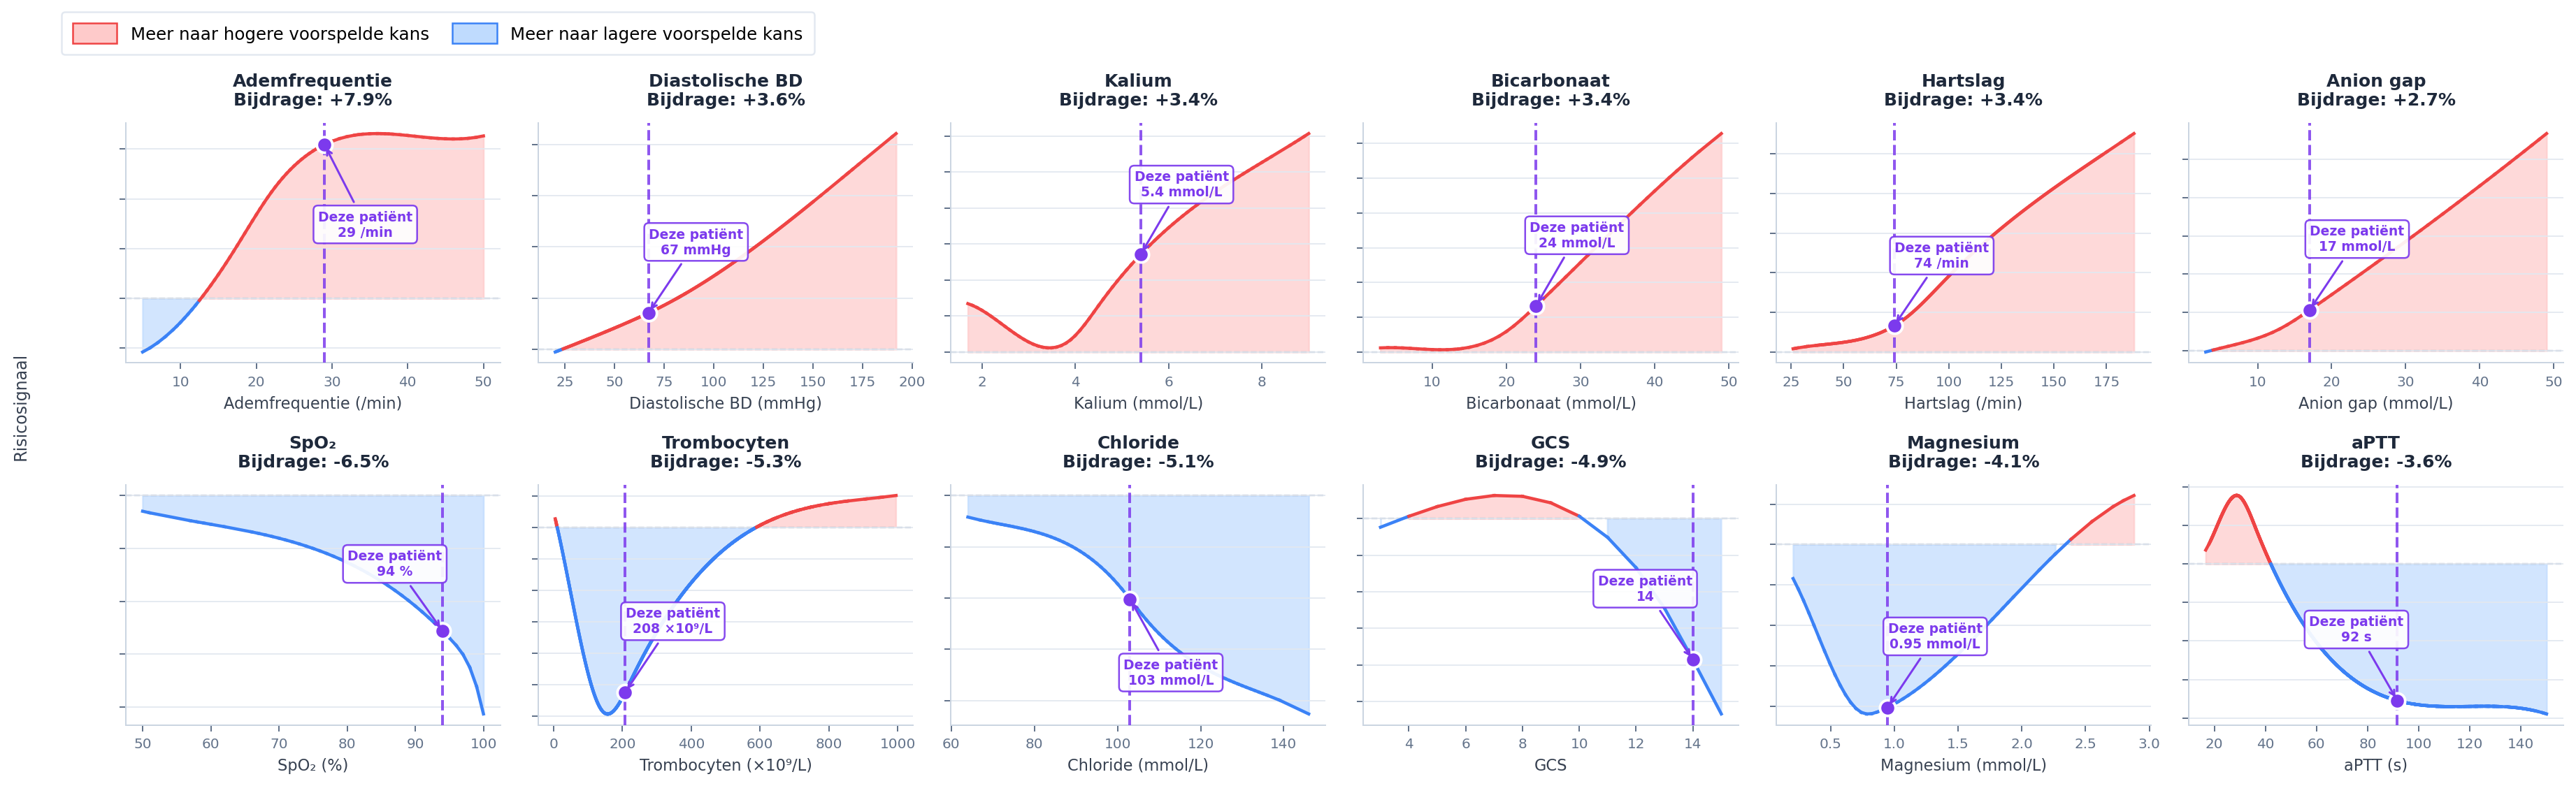
\includegraphics[width=\textwidth]{SupplementaryImages/12-panelSpline.png}
  \caption{Twelve-panel spline chart sent as PNG to the LLM and shown to Group~B participants.}
  \label{fig:12panel}
\end{figure}

\end{document}
